
\documentclass[12pt, a4paper]{article}
\usepackage{xeCJK} % Support for Chinese characters
\setCJKmainfont{Noto Sans TC} % Traditional Chinese Sans-serif (NotoSansTC-VF.ttf)
\setCJKmonofont{Noto Sans TC}
\usepackage{geometry}
\geometry{left=2.5cm, right=2.5cm, top=2.5cm, bottom=2.5cm}
\usepackage{graphicx}
\usepackage{float}
\usepackage{booktabs}
\usepackage{listings}
\usepackage{xcolor}
\usepackage{hyperref}
\usepackage{longtable}
\usepackage{caption}

% Define colors for code listing
\definecolor{codegreen}{rgb}{0,0.6,0}
\definecolor{codegray}{rgb}{0.5,0.5,0.5}
\definecolor{codepurple}{rgb}{0.58,0,0.82}
\definecolor{backcolour}{rgb}{0.95,0.95,0.92}

\lstdefinestyle{vhdlstyle}{
    backgroundcolor=\color{backcolour},
    commentstyle=\color{codegreen},
    keywordstyle=\color{magenta},
    numberstyle=\tiny\color{codegray},
    stringstyle=\color{codepurple},
    basicstyle=\ttfamily\footnotesize,
    breakatwhitespace=false,
    breaklines=true,
    captionpos=b,
    keepspaces=true,
    numbers=left,
    numbersep=5pt,
    showspaces=false,
    showstringspaces=false,
    showtabs=false,
    tabsize=2,
    language=VHDL
}

\title{微處理器系統實驗報告 - Lab 07}
\author{資工二 \\ 113590051 楊承諭 \\ 113590017 黃楷程}
\date{2026年5月29日}

\begin{document}

\maketitle
\hrule

\section*{實驗基本資訊}
\begin{itemize}
    \item \textbf{系級：} 資工二
    \item \textbf{學號/姓名：} 113590051 / 楊承諭、113590017 / 黃楷程
    \item \textbf{日期：} 2026/05/29
    \item \textbf{實驗名稱：} 八位元除法器 (8-Bit Restoring Divider) 硬體設計
\end{itemize}

\hrule

\section*{組員貢獻比例}
\begin{table}[H]
    \centering
    \begin{tabular}{@{}llll@{}}
        \toprule
        \textbf{姓名} & \textbf{學號} & \textbf{貢獻比例} & \textbf{負責內容} \\ \midrule
        楊承諭 & 113590051 & 100\% & 小組專案製作與小組報告製作 \\
        黃楷程 & 113590017 & 0\%   & 無貢獻內容 \\ \bottomrule
    \end{tabular}
\end{table}

\section{實驗內容}

本次實驗的主題為「八位元恢復除法器 (8-Bit Restoring Divider) 之硬體設計」。實驗目標是使用 VHDL 語言在 FPGA 開發板 (Altera DE2-115) 上，以「結構化 (Structural)」架構實現一個完整的 8 位元二進位除法器，包含資料路徑 (Datapath) 與控制器 (Controller) 兩大部分。

\subsection{實驗目標}
\begin{enumerate}
    \item 理解恢復除法演算法 (Restoring Division Algorithm) 的數學原理與流程。
    \item 設計並整合一個六狀態的有限狀態機 (FSM) 作為控制器，依序驅動各暫存器的運算。
    \item 重複使用 Lab 05 中設計的泛用移位暫存器 (\texttt{N\_bit\_DFF}) 作為商數 (Q)、除數 (D) 及餘數 (R) 三個暫存器的元件，充分體現硬體的模組化設計精神。
    \item 在運算完成後 (S4 狀態)，透過四個七段顯示器 (HEX3 \textasciitilde\ HEX0) 以十六進位顯示最終的商與餘數。
\end{enumerate}

\subsection{硬體架構概述}

整體設計分為以下兩層架構：

\begin{itemize}
    \item \textbf{資料路徑 (Datapath)：} 由三個以 \texttt{n\_bit\_DFF} 泛型實例化的暫存器構成。
    \begin{itemize}
        \item \textbf{Q 暫存器（商數，8-bit）：} 用於累積商數位元，每次迭代向左移位並串入 \texttt{sdi\_Q}（S2a 串入 '1'，S2b 串入 '0'）。
        \item \textbf{D 暫存器（除數，17-bit）：} 初始載入除數於高位元組（位元 15:8），每次 S3 狀態向右移一位，模擬二進位對齊。
        \item \textbf{R 暫存器（餘數，17-bit）：} 初始載入被除數於低位元組（位元 7:0），每次 S1 載入減法結果，S2b 時恢復 (\texttt{R + D})。
    \end{itemize}
    \item \textbf{組合邏輯 ALU：} 一個 17-bit 減法器（\texttt{sub\_res <= qo\_R - qo\_D}），其最高符號位元 (\texttt{sub\_res(16)}) 決定 FSM 由 S1 跳轉至 S2a 或 S2b。
\end{itemize}

\subsection{腳位分配 (Pin Assignment)}

\begin{table}[H]
    \centering
    \caption{FPGA 腳位分配表}
    \begin{tabular}{@{}llll@{}}
        \toprule
        \textbf{訊號名稱} & \textbf{方向} & \textbf{FPGA 腳位} & \textbf{功能描述} \\ \midrule
        Clock     & in  & PIN\_M23 (KEY[0])      & 系統時脈（手動步進按鍵） \\
        Reset     & in  & PIN\_Y24 (SW[16])      & 非同步重置，重回 Start 狀態 \\
        Divisor   & in  & SW[7..0]               & 8-bit 除數輸入 \\
        Dividend  & in  & SW[15..8]              & 8-bit 被除數輸入 \\
        Quotient  & out & LEDR[7..0]             & 即時商數 LED 顯示 \\
        Remainder & out & LEDR[15..8]            & 即時餘數 LED 顯示 \\
        HEX0      & out & HEX0[6..0]             & 最終商數低位 nibble（七段顯示）\\
        HEX1      & out & HEX1[6..0]             & 最終商數高位 nibble（七段顯示）\\
        HEX2      & out & HEX2[6..0]             & 最終餘數低位 nibble（七段顯示）\\
        HEX3      & out & HEX3[6..0]             & 最終餘數高位 nibble（七段顯示）\\ \bottomrule
    \end{tabular}
\end{table}

\section{邏輯設計與實驗過程}

\subsection{恢復除法演算法說明}

恢復除法演算法是一種基於逐位元 (bit-by-bit) 試減的二進位除法方法，其核心思想為：

\begin{enumerate}
    \item \textbf{初始化（Start）：} 將除數 $B$ 載入 D 暫存器高位元組，被除數 $A$ 載入 R 暫存器低位元組，Q 暫存器清零。
    \item \textbf{試減（S1）：} 計算 $R - D$，若結果 $\geq 0$（符號位元為 0），進入 S2a；否則進入 S2b。
    \item \textbf{S2a（不恢復）：} 餘數更新為減法結果，Q 左移並串入 '1'。
    \item \textbf{S2b（恢復）：} 餘數恢復為 $R + D$，Q 左移並串入 '0'。
    \item \textbf{移位計數（S3）：} D 暫存器右移一位（相當於除數位元對齊下移）。若已完成 9 次迭代，進入 S4；否則回到 S1。
    \item \textbf{完成（S4）：} 凍結所有暫存器，於七段顯示器顯示最終商與餘數。
\end{enumerate}

\subsection{有限狀態機 (FSM) 狀態轉移}

\begin{table}[H]
    \centering
    \caption{FSM 狀態轉移表}
    \begin{tabular}{@{}lll@{}}
        \toprule
        \textbf{現在狀態} & \textbf{條件} & \textbf{下一狀態} \\ \midrule
        Start  & Reset 解除後第一個時脈觸發 & S1 \\
        S1     & \texttt{sub\_res(16) = '0'}（結果 $\geq 0$） & S2a \\
        S1     & \texttt{sub\_res(16) = '1'}（結果 $< 0$）    & S2b \\
        S2a    & 無條件 & S3 \\
        S2b    & 無條件 & S3 \\
        S3     & \texttt{count < 8} & S1（繼續迭代）\\
        S3     & \texttt{count = 8} & S4（完成）\\
        S4     & 無條件（直到 Reset） & S4 \\
        \bottomrule
    \end{tabular}
\end{table}

\subsection{實驗步驟}
\begin{itemize}
    \item 在 Quartus 中建立專案，加入 \texttt{Division.vhd} 與 \texttt{N\_bit\_DFF.vhd} 兩個設計檔案，並設定 \texttt{Division} 為頂層模組。
    \item 進行編譯與合成，確認無語法及邏輯錯誤。
    \item 依照腳位分配表完成 Pin Assignment，設定 SW[15..0]、KEY[0]、SW[16]、LEDR[15..0] 及 HEX[3..0] 腳位。
    \item 將設計燒錄至 DE2-115 開發板，設定 SW[15..8]（被除數）與 SW[7..0]（除數），然後透過 SW[16] 進行 Reset，再以手動按壓 KEY[0] 逐步驅動 FSM 進行除法運算。
    \item 驗證 LED 與七段顯示器的輸出是否正確。
\end{itemize}

\section{實驗結果（照片紀錄）}

以下照片記錄了在 DE2-115 開發板上驗證 8 位元除法器的完整過程，測試案例為 $A \div B = 65 \div 13 = 5\ldots0$（即 \texttt{0x41} $\div$ \texttt{0x0D} = \texttt{0x05} 餘 \texttt{0x00}）。

\begin{figure}[H]
    \centering
    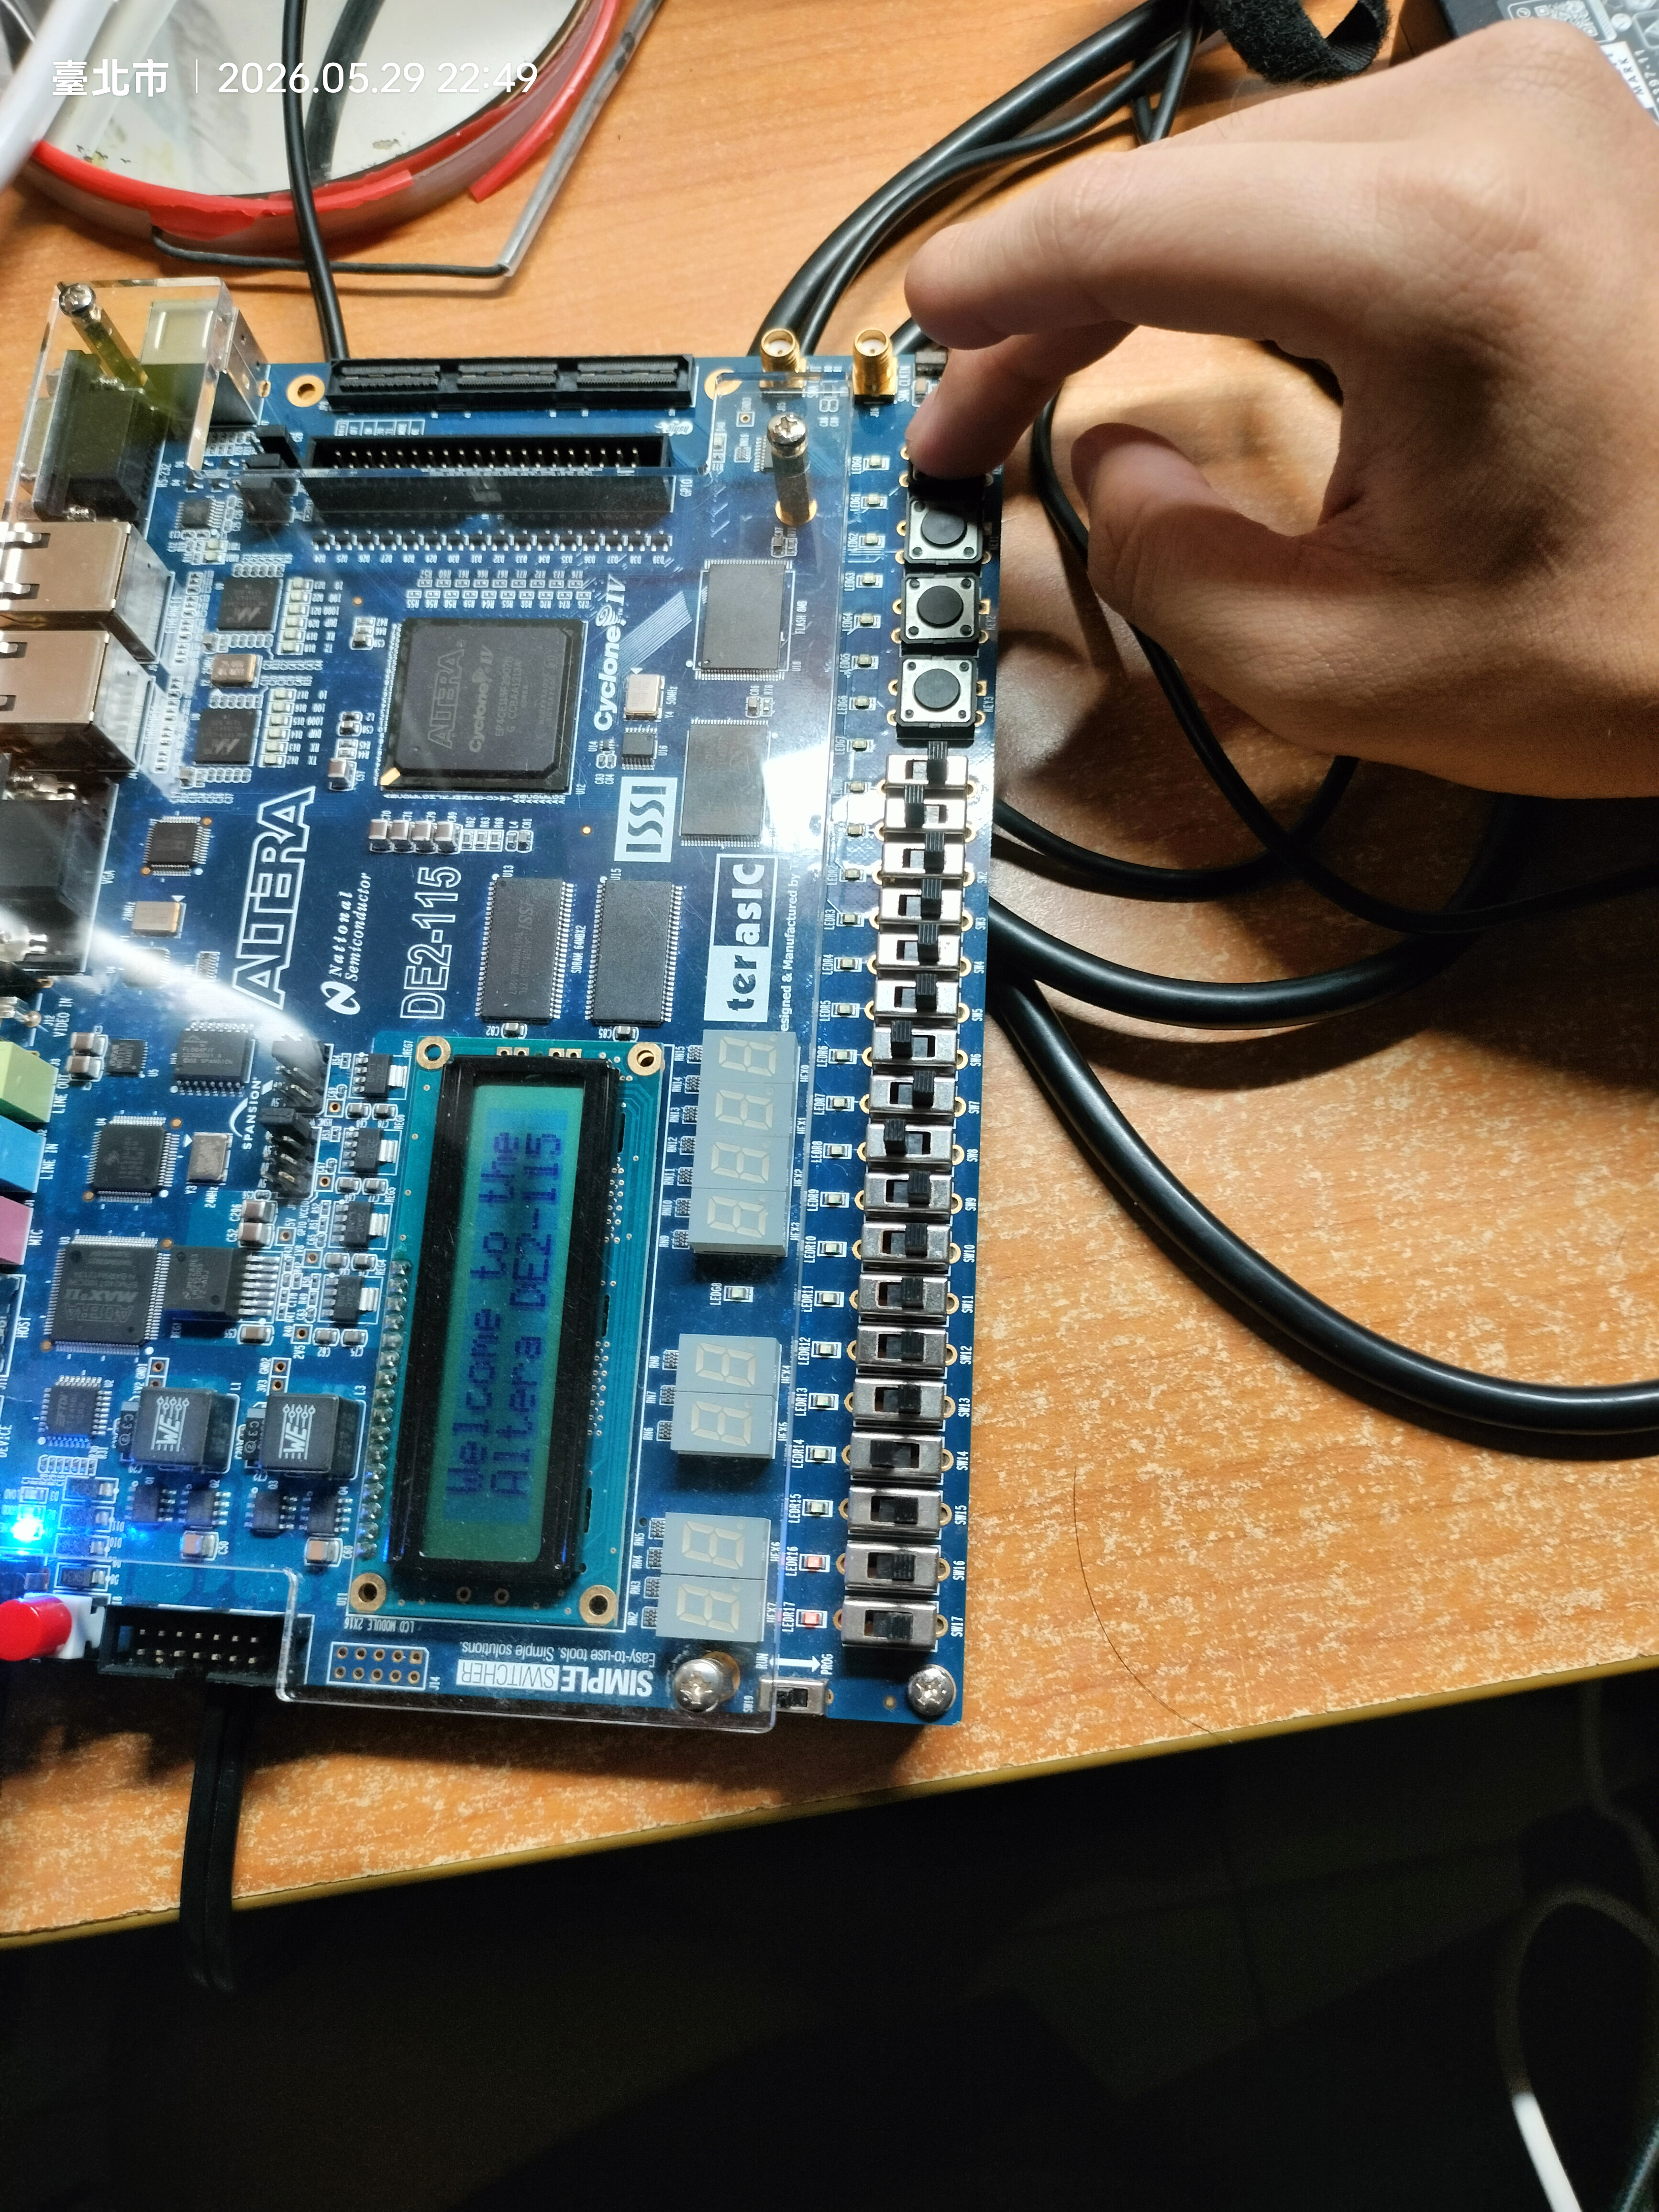
\includegraphics[width=0.65\textwidth]{../../photo/IMG20260529224923.jpg}
    \caption{初始狀態（Start）：SW[16] 撥高完成 Reset，所有 LED 熄滅，七段顯示空白，準備開始除法運算。}
\end{figure}

\begin{figure}[H]
    \centering
    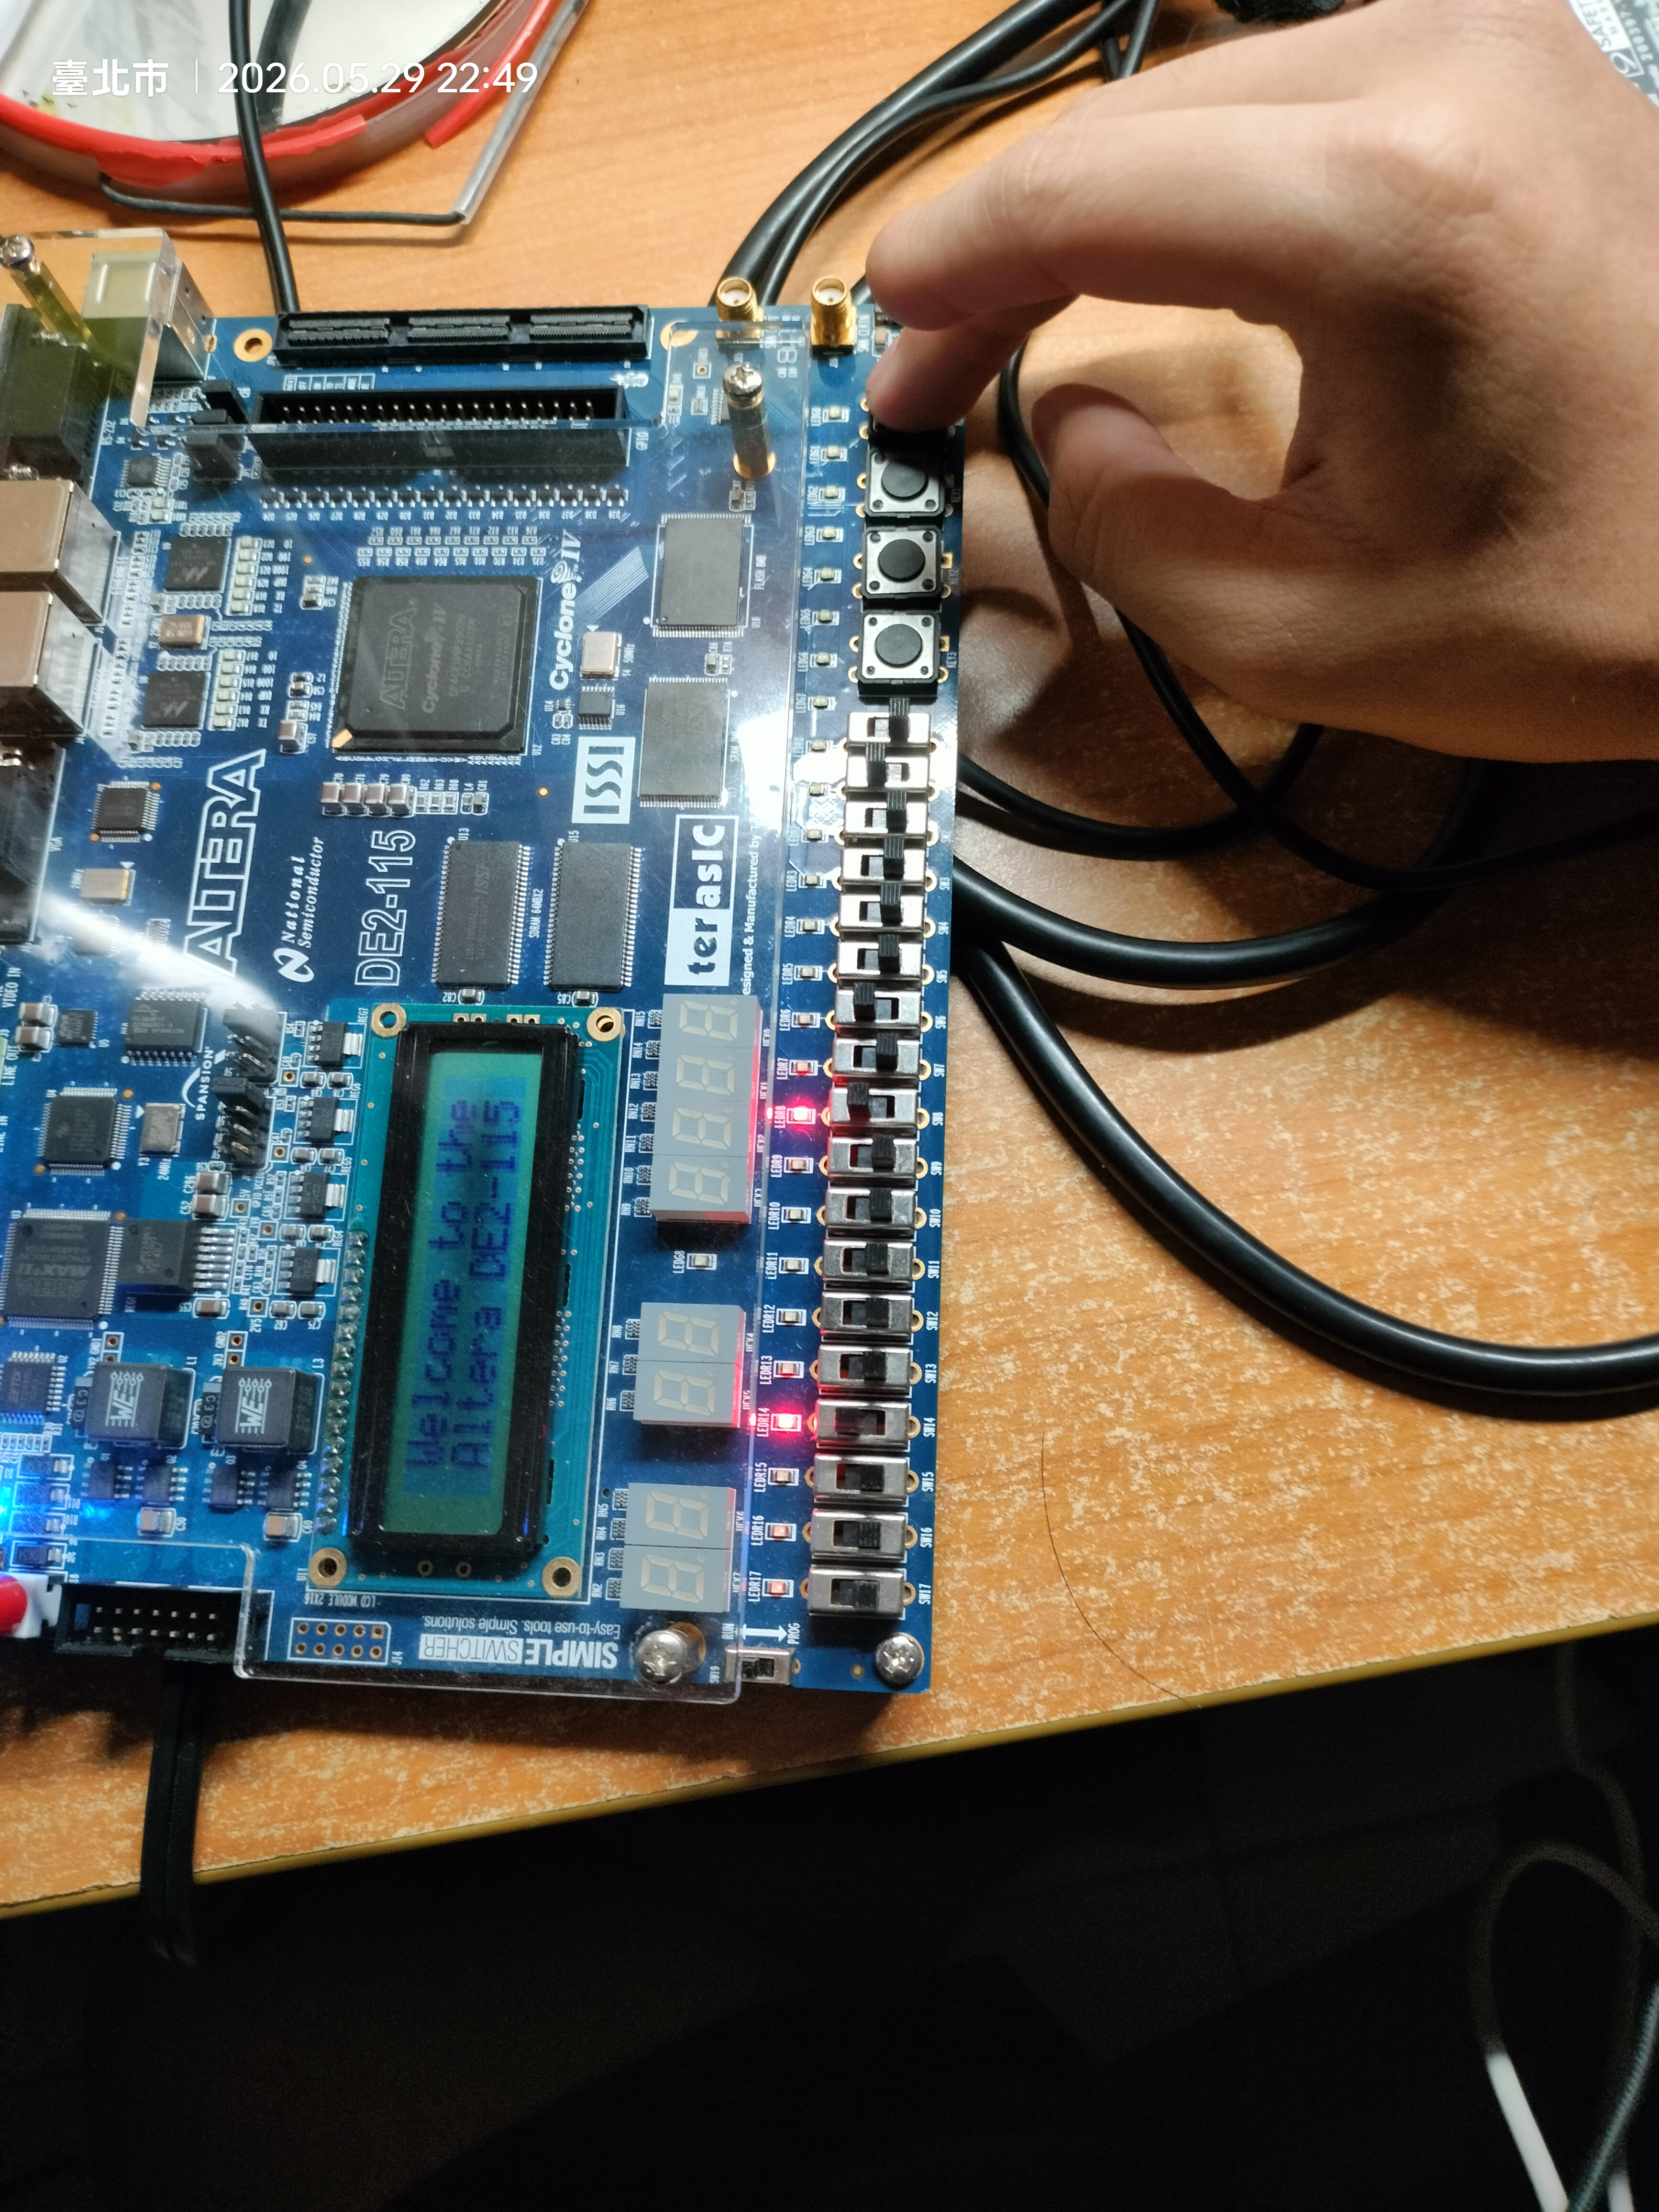
\includegraphics[width=0.65\textwidth]{../../photo/IMG20260529224925.jpg}
    \caption{輸入被除數與除數：SW[15..8] 設定被除數，SW[7..0] 設定除數，確認撥碼開關設定正確。}
\end{figure}

\begin{figure}[H]
    \centering
    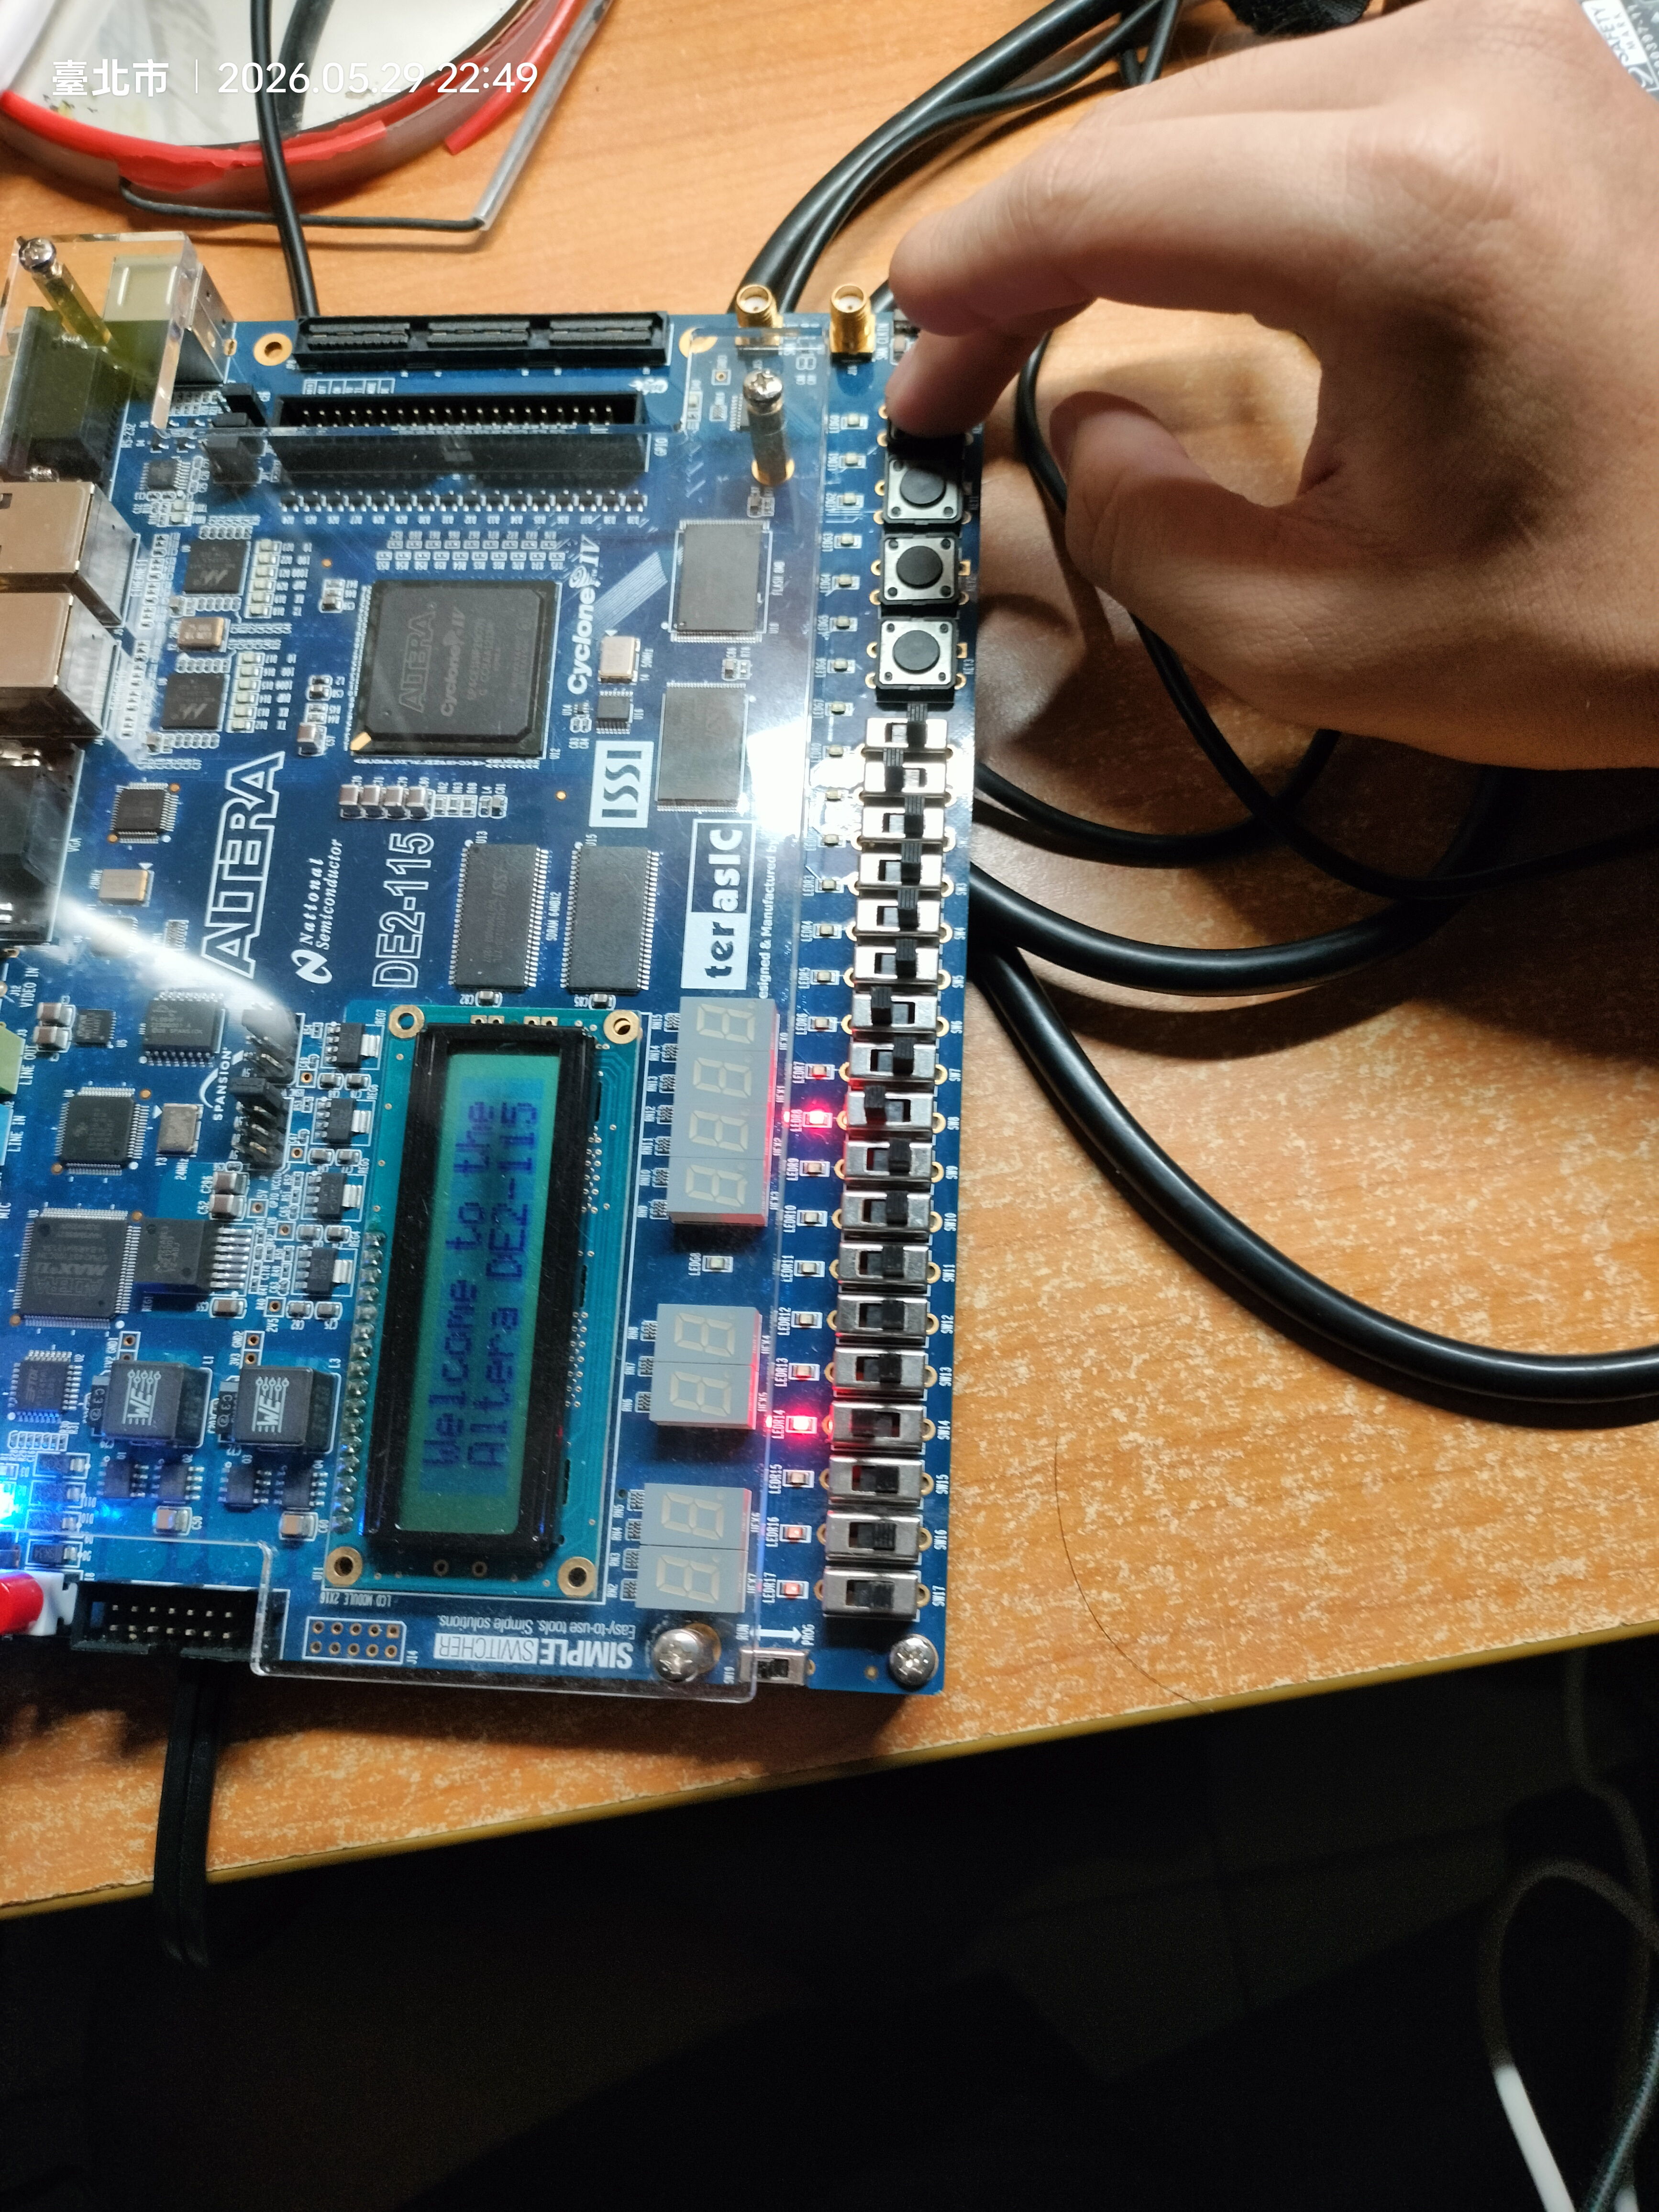
\includegraphics[width=0.65\textwidth]{../../photo/IMG20260529224927.jpg}
    \caption{按下 KEY[0] 第一次：FSM 從 Start 進入 S1，R 暫存器執行試減，LED 顯示目前餘數狀態。}
\end{figure}

\begin{figure}[H]
    \centering
    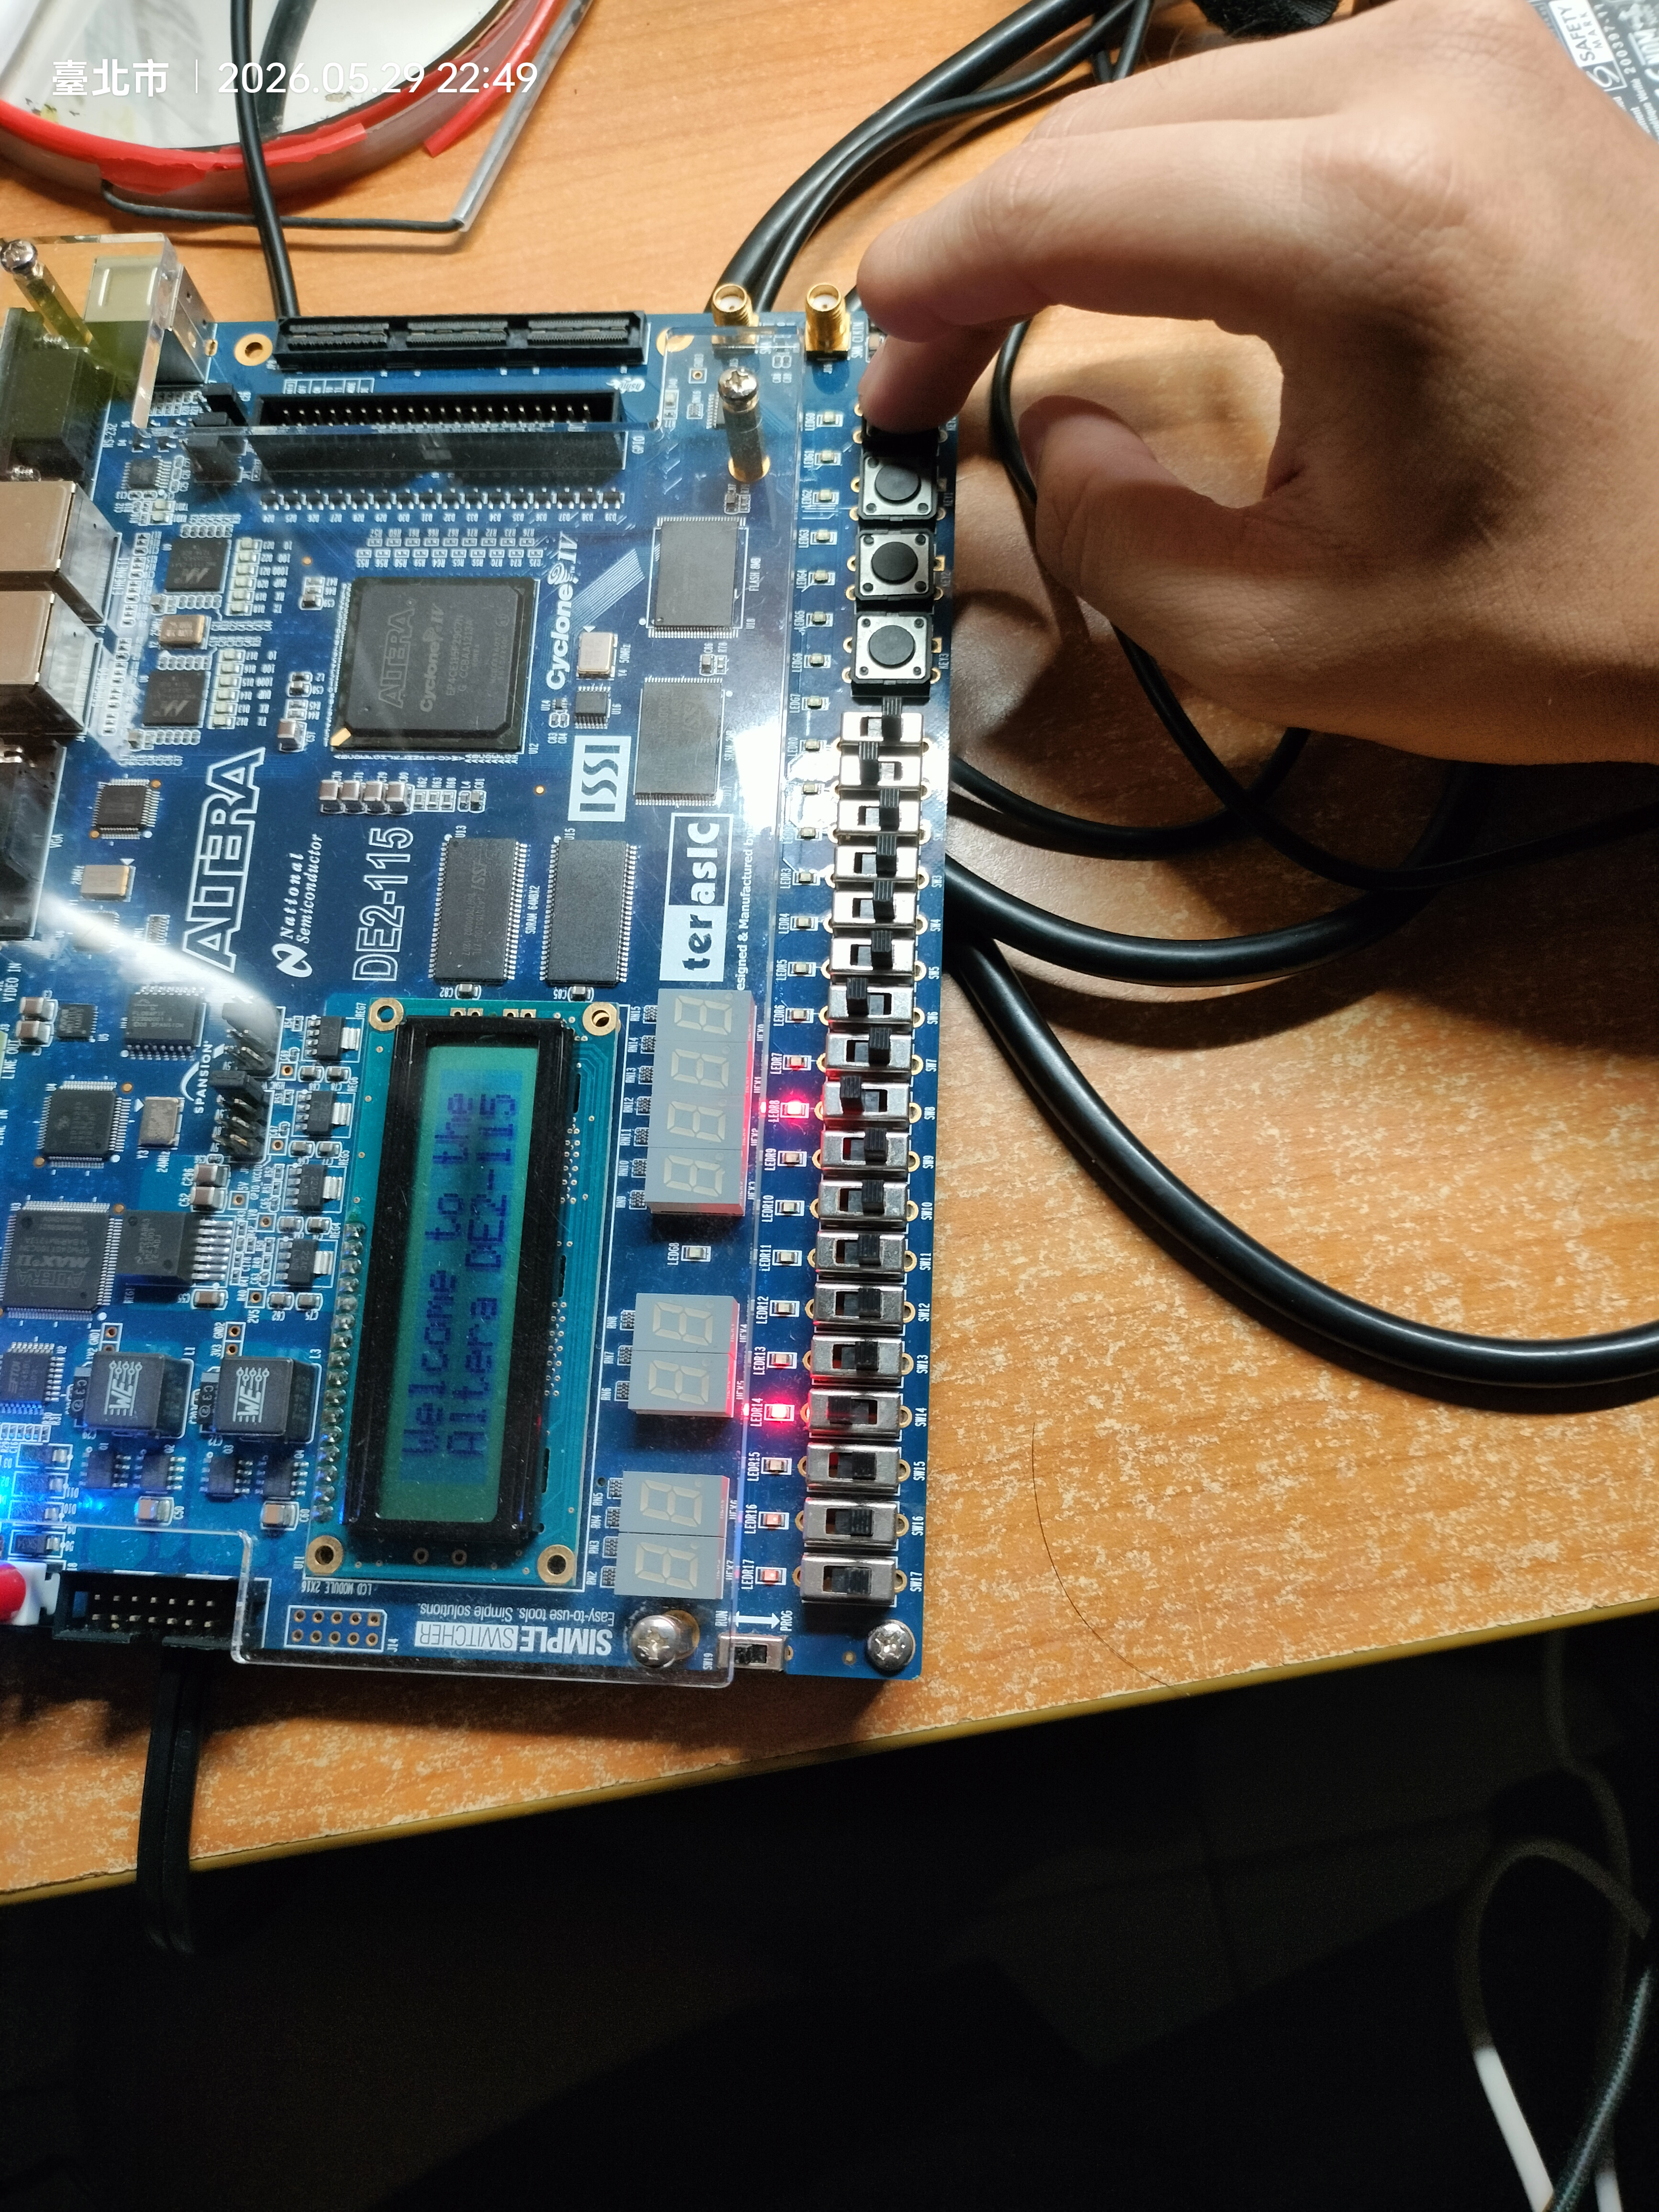
\includegraphics[width=0.65\textwidth]{../../photo/IMG20260529224928.jpg}
    \caption{FSM 進入 S2a（餘數非負）：商數暫存器左移並串入 '1'，LED 顯示商數中間運算過程。}
\end{figure}

\begin{figure}[H]
    \centering
    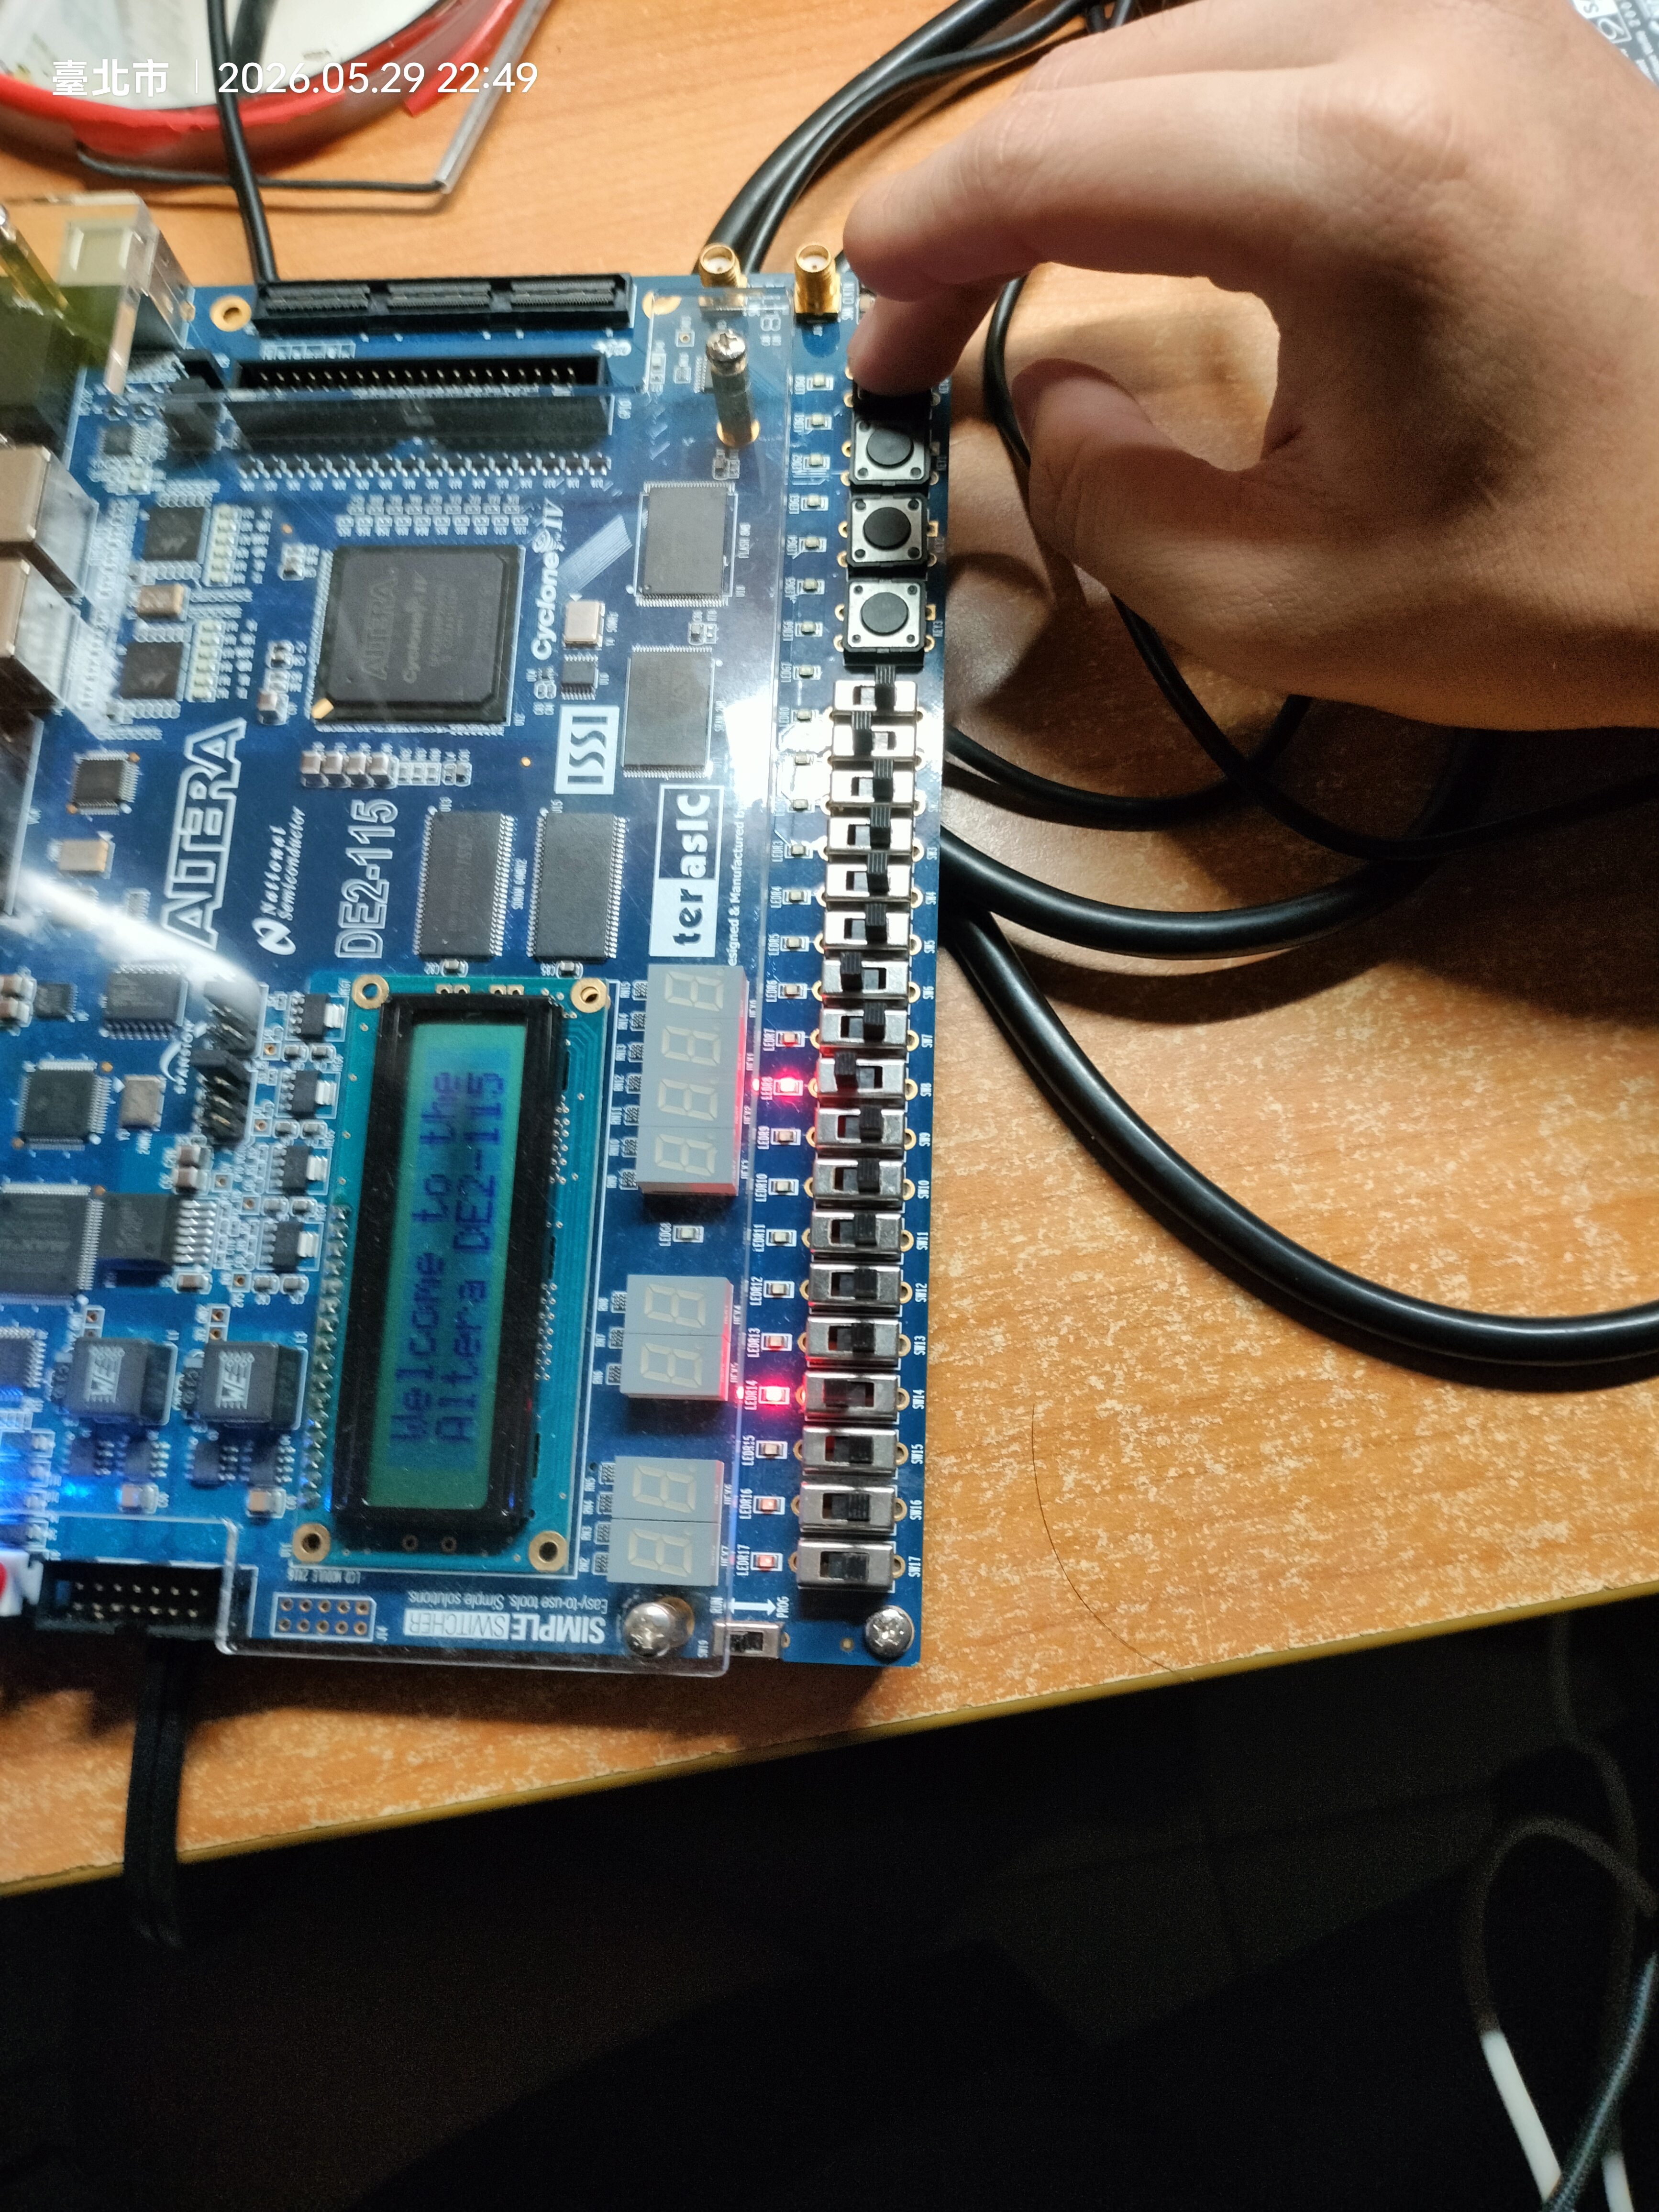
\includegraphics[width=0.65\textwidth]{../../photo/IMG20260529224930.jpg}
    \caption{FSM 進入 S3：除數暫存器右移一位，計數器遞增，準備進行下一輪迭代。}
\end{figure}

\begin{figure}[H]
    \centering
    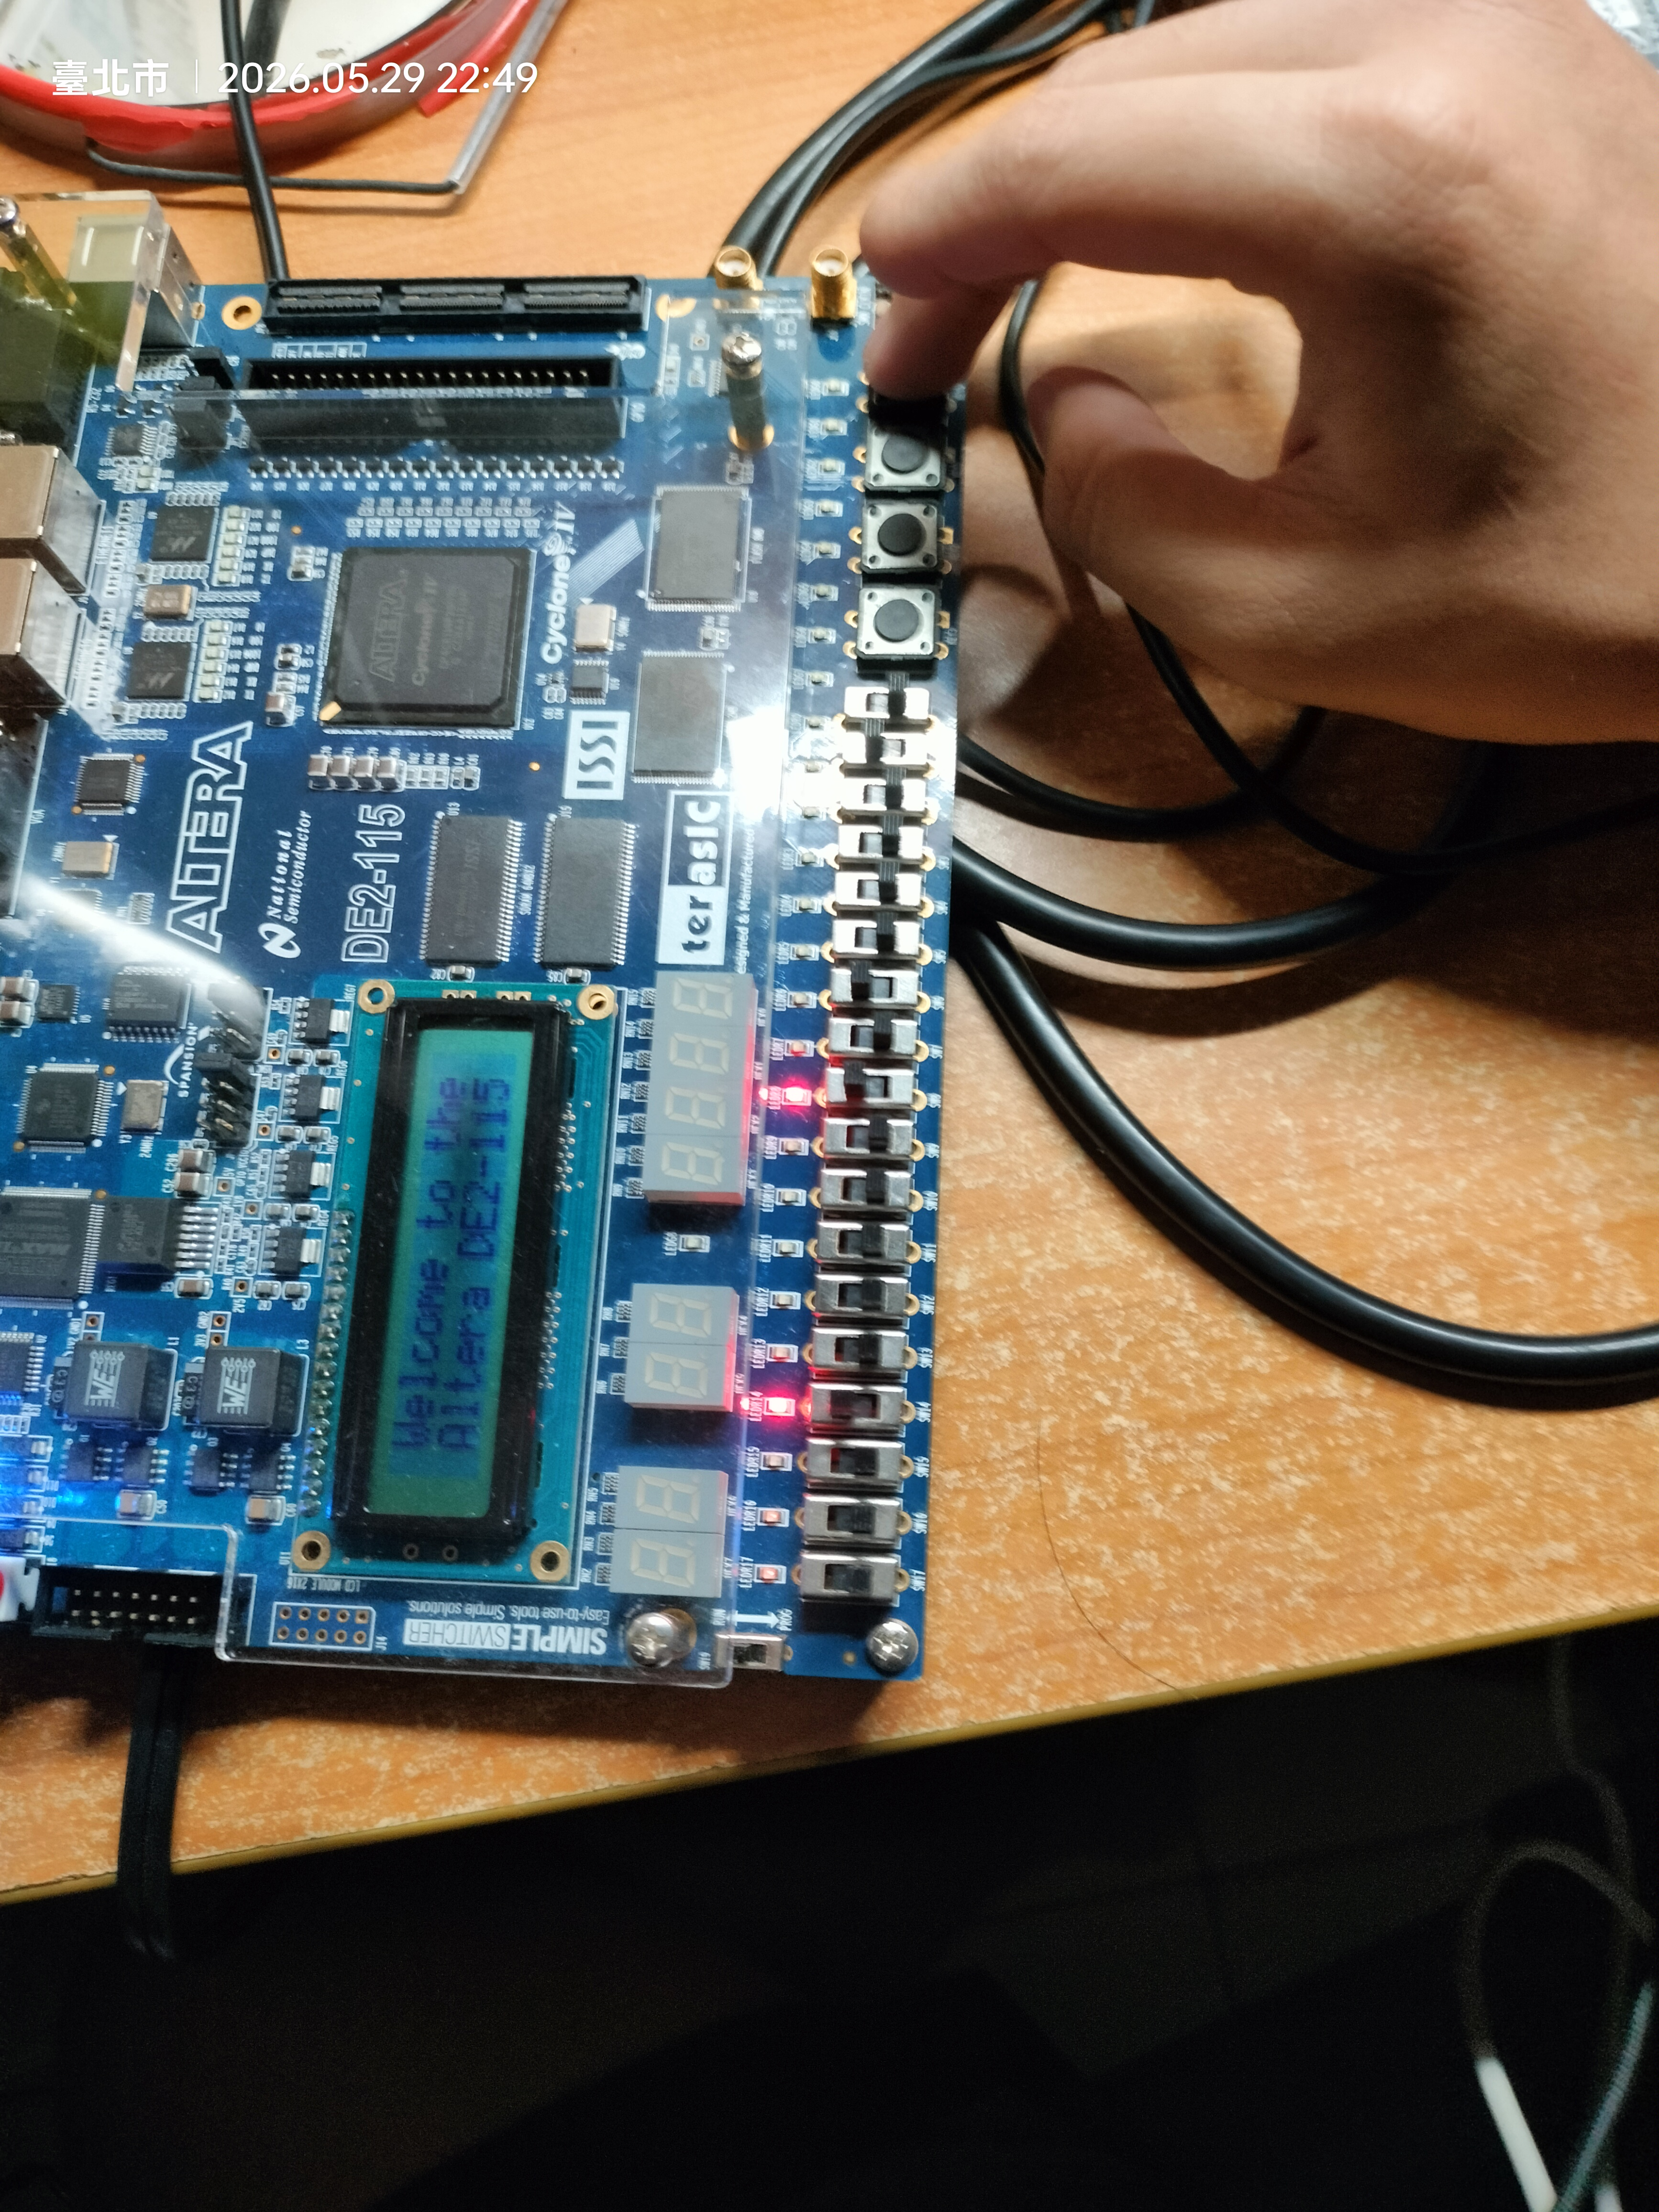
\includegraphics[width=0.65\textwidth]{../../photo/IMG20260529224932.jpg}
    \caption{迭代過程中 FSM 進入 S2b（餘數為負）：執行餘數恢復操作（R = R + D），商數左移串入 '0'。}
\end{figure}

\begin{figure}[H]
    \centering
    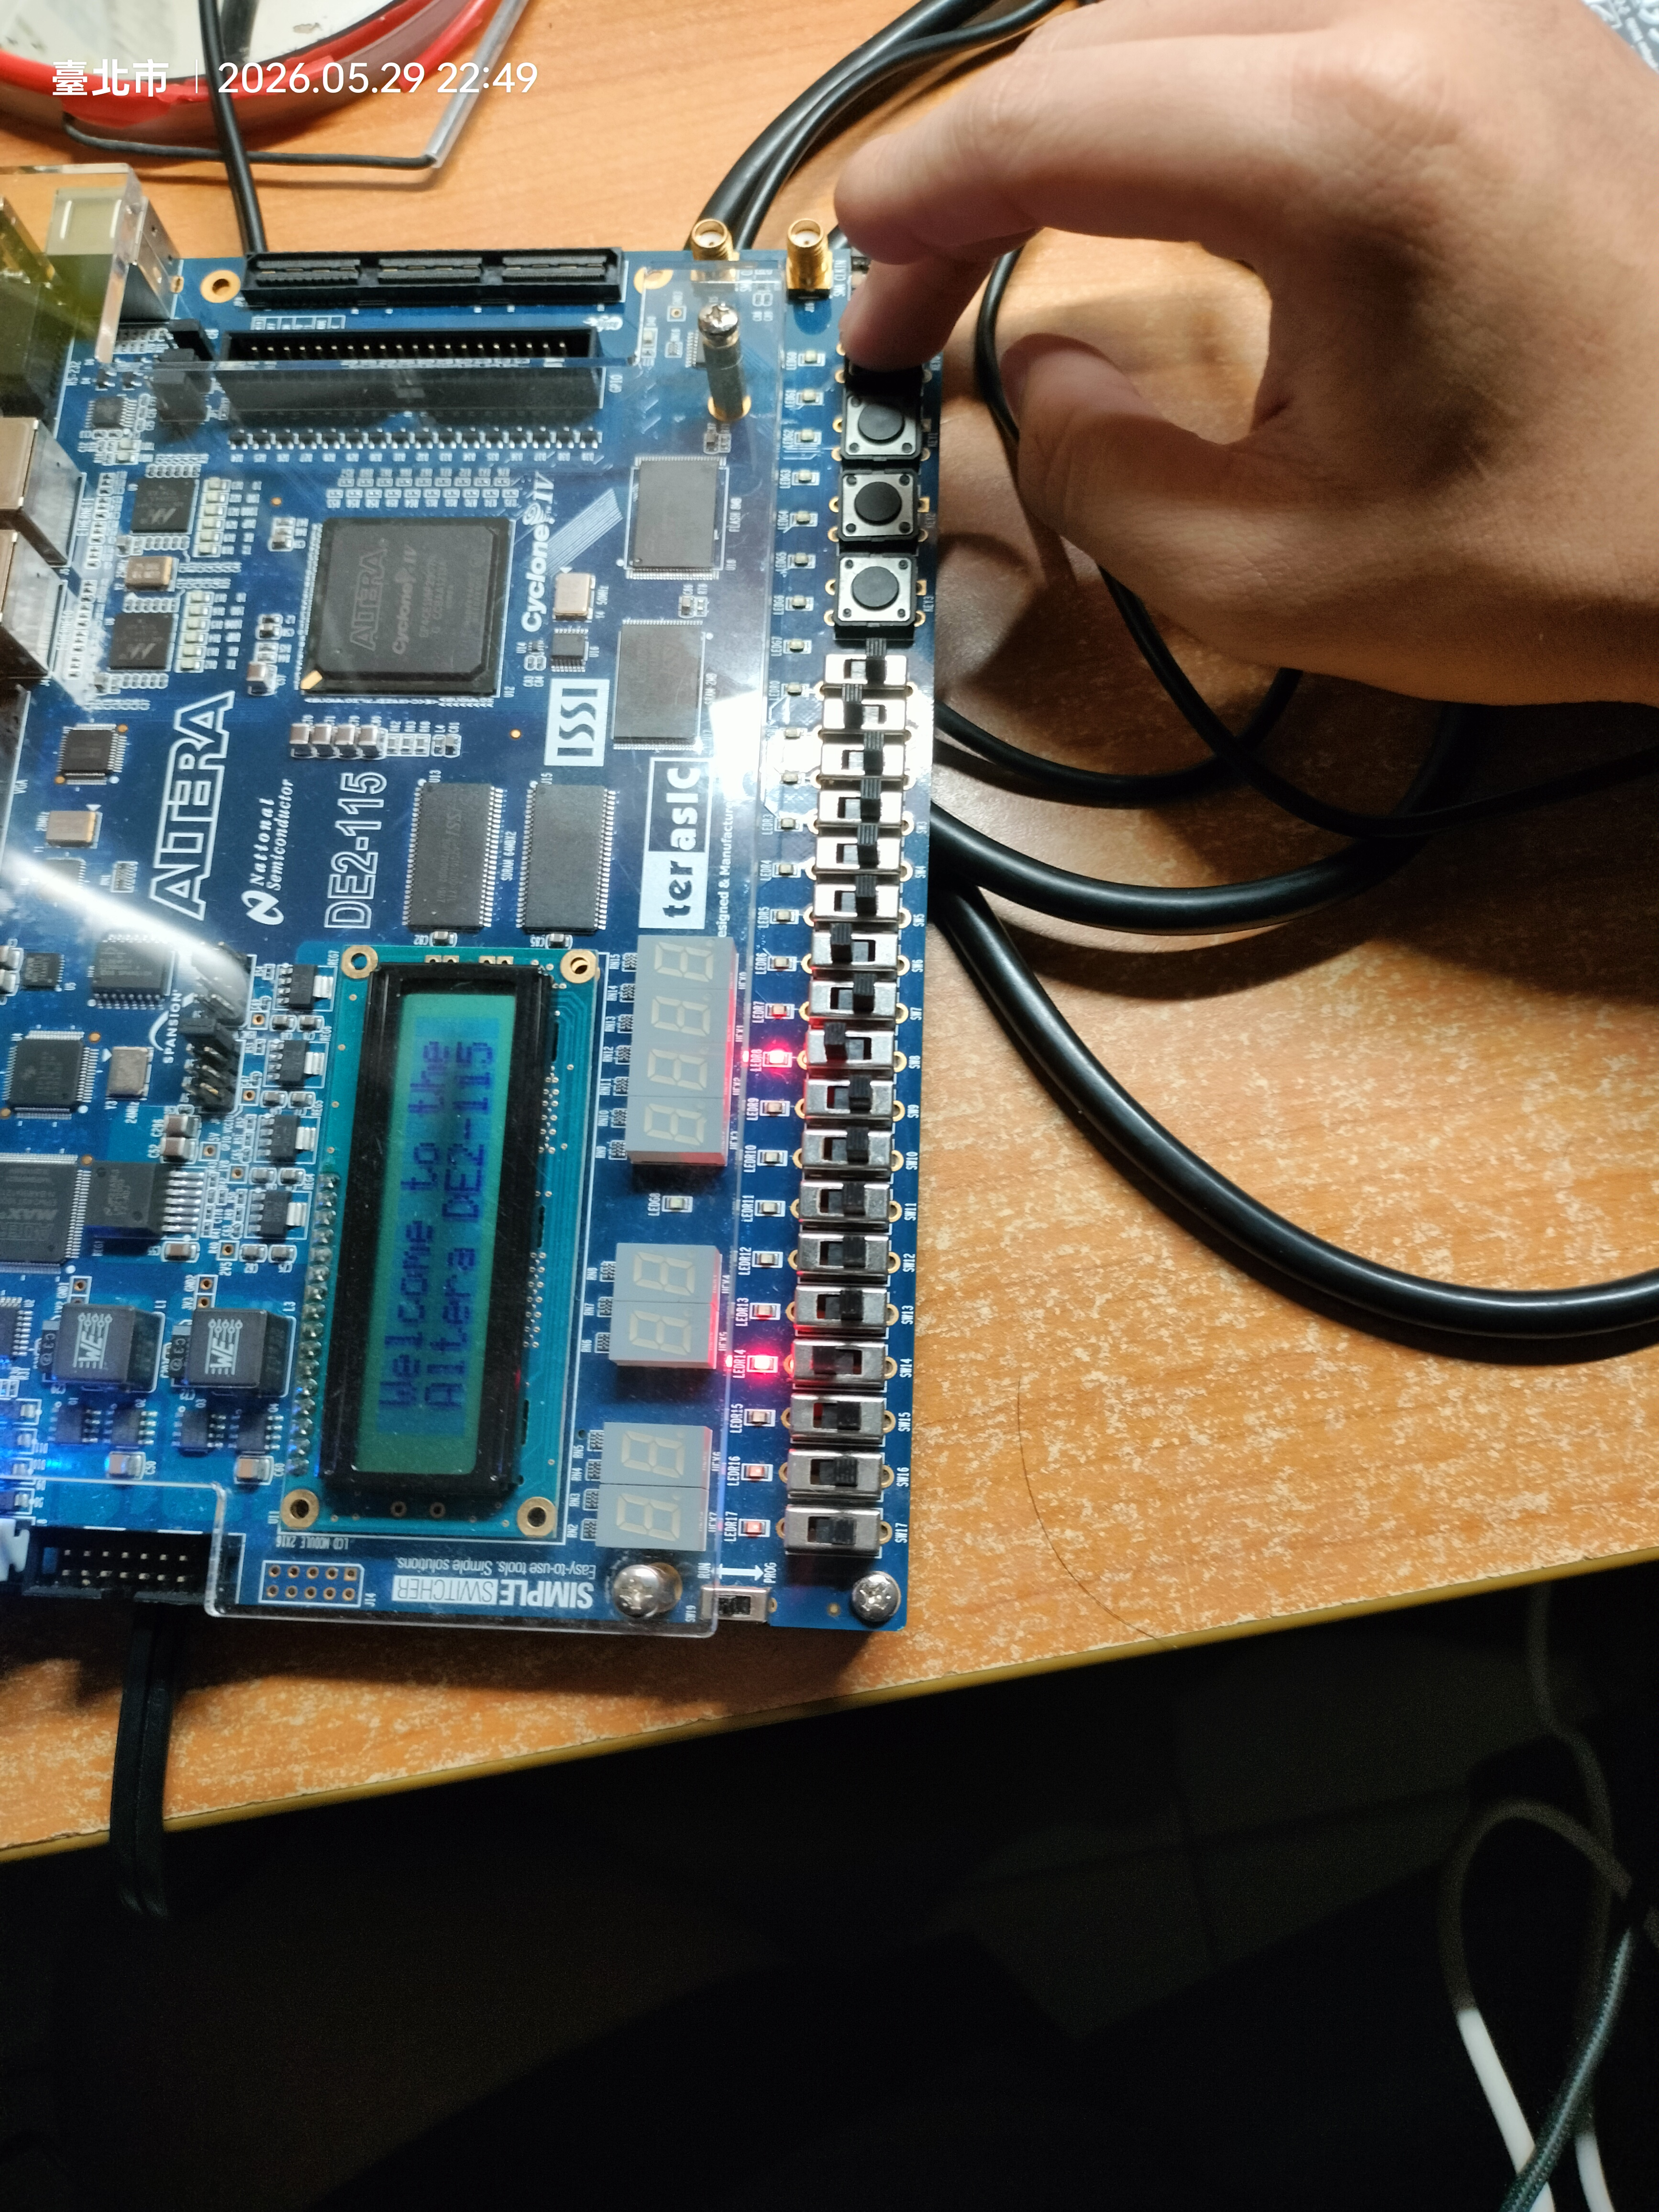
\includegraphics[width=0.65\textwidth]{../../photo/IMG20260529224933.jpg}
    \caption{持續按壓 KEY[0] 逐步執行迭代：LED 顯示各迭代步驟中商數與餘數的中間值。}
\end{figure}

\begin{figure}[H]
    \centering
    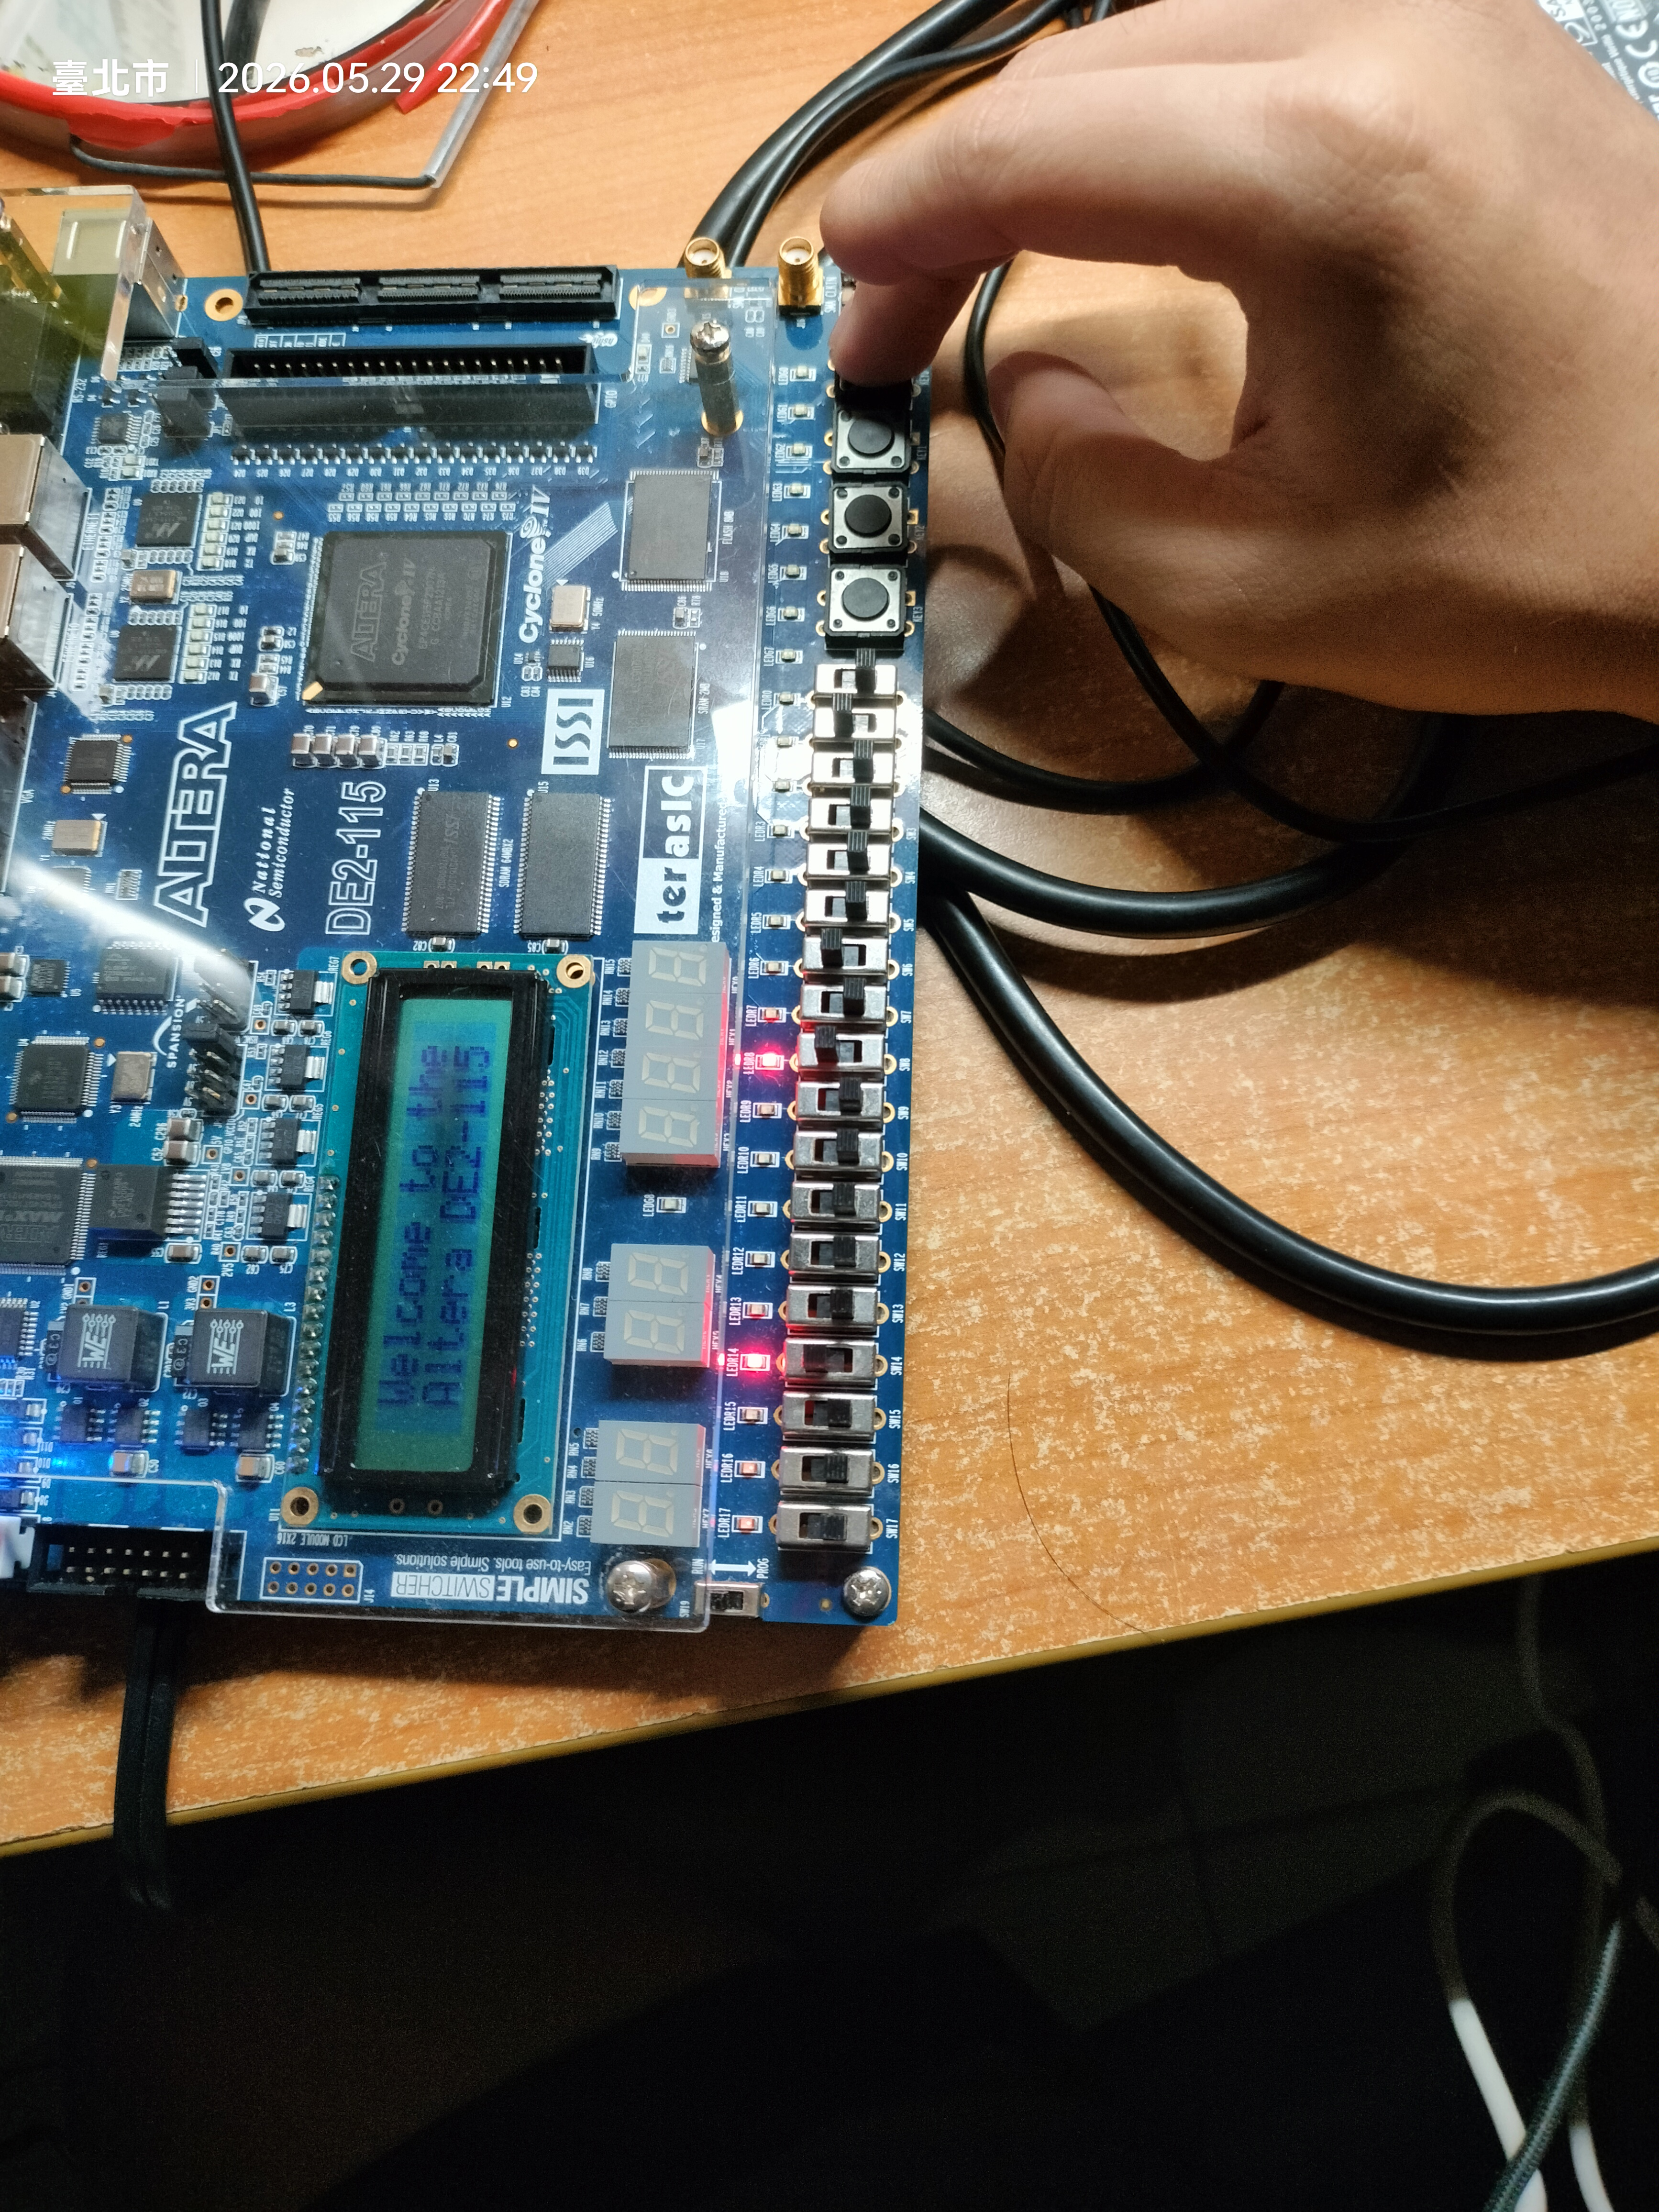
\includegraphics[width=0.65\textwidth]{../../photo/IMG20260529224935.jpg}
    \caption{第 8 次迭代中的 S1 狀態：FSM 執行最後一次試減操作。}
\end{figure}

\begin{figure}[H]
    \centering
    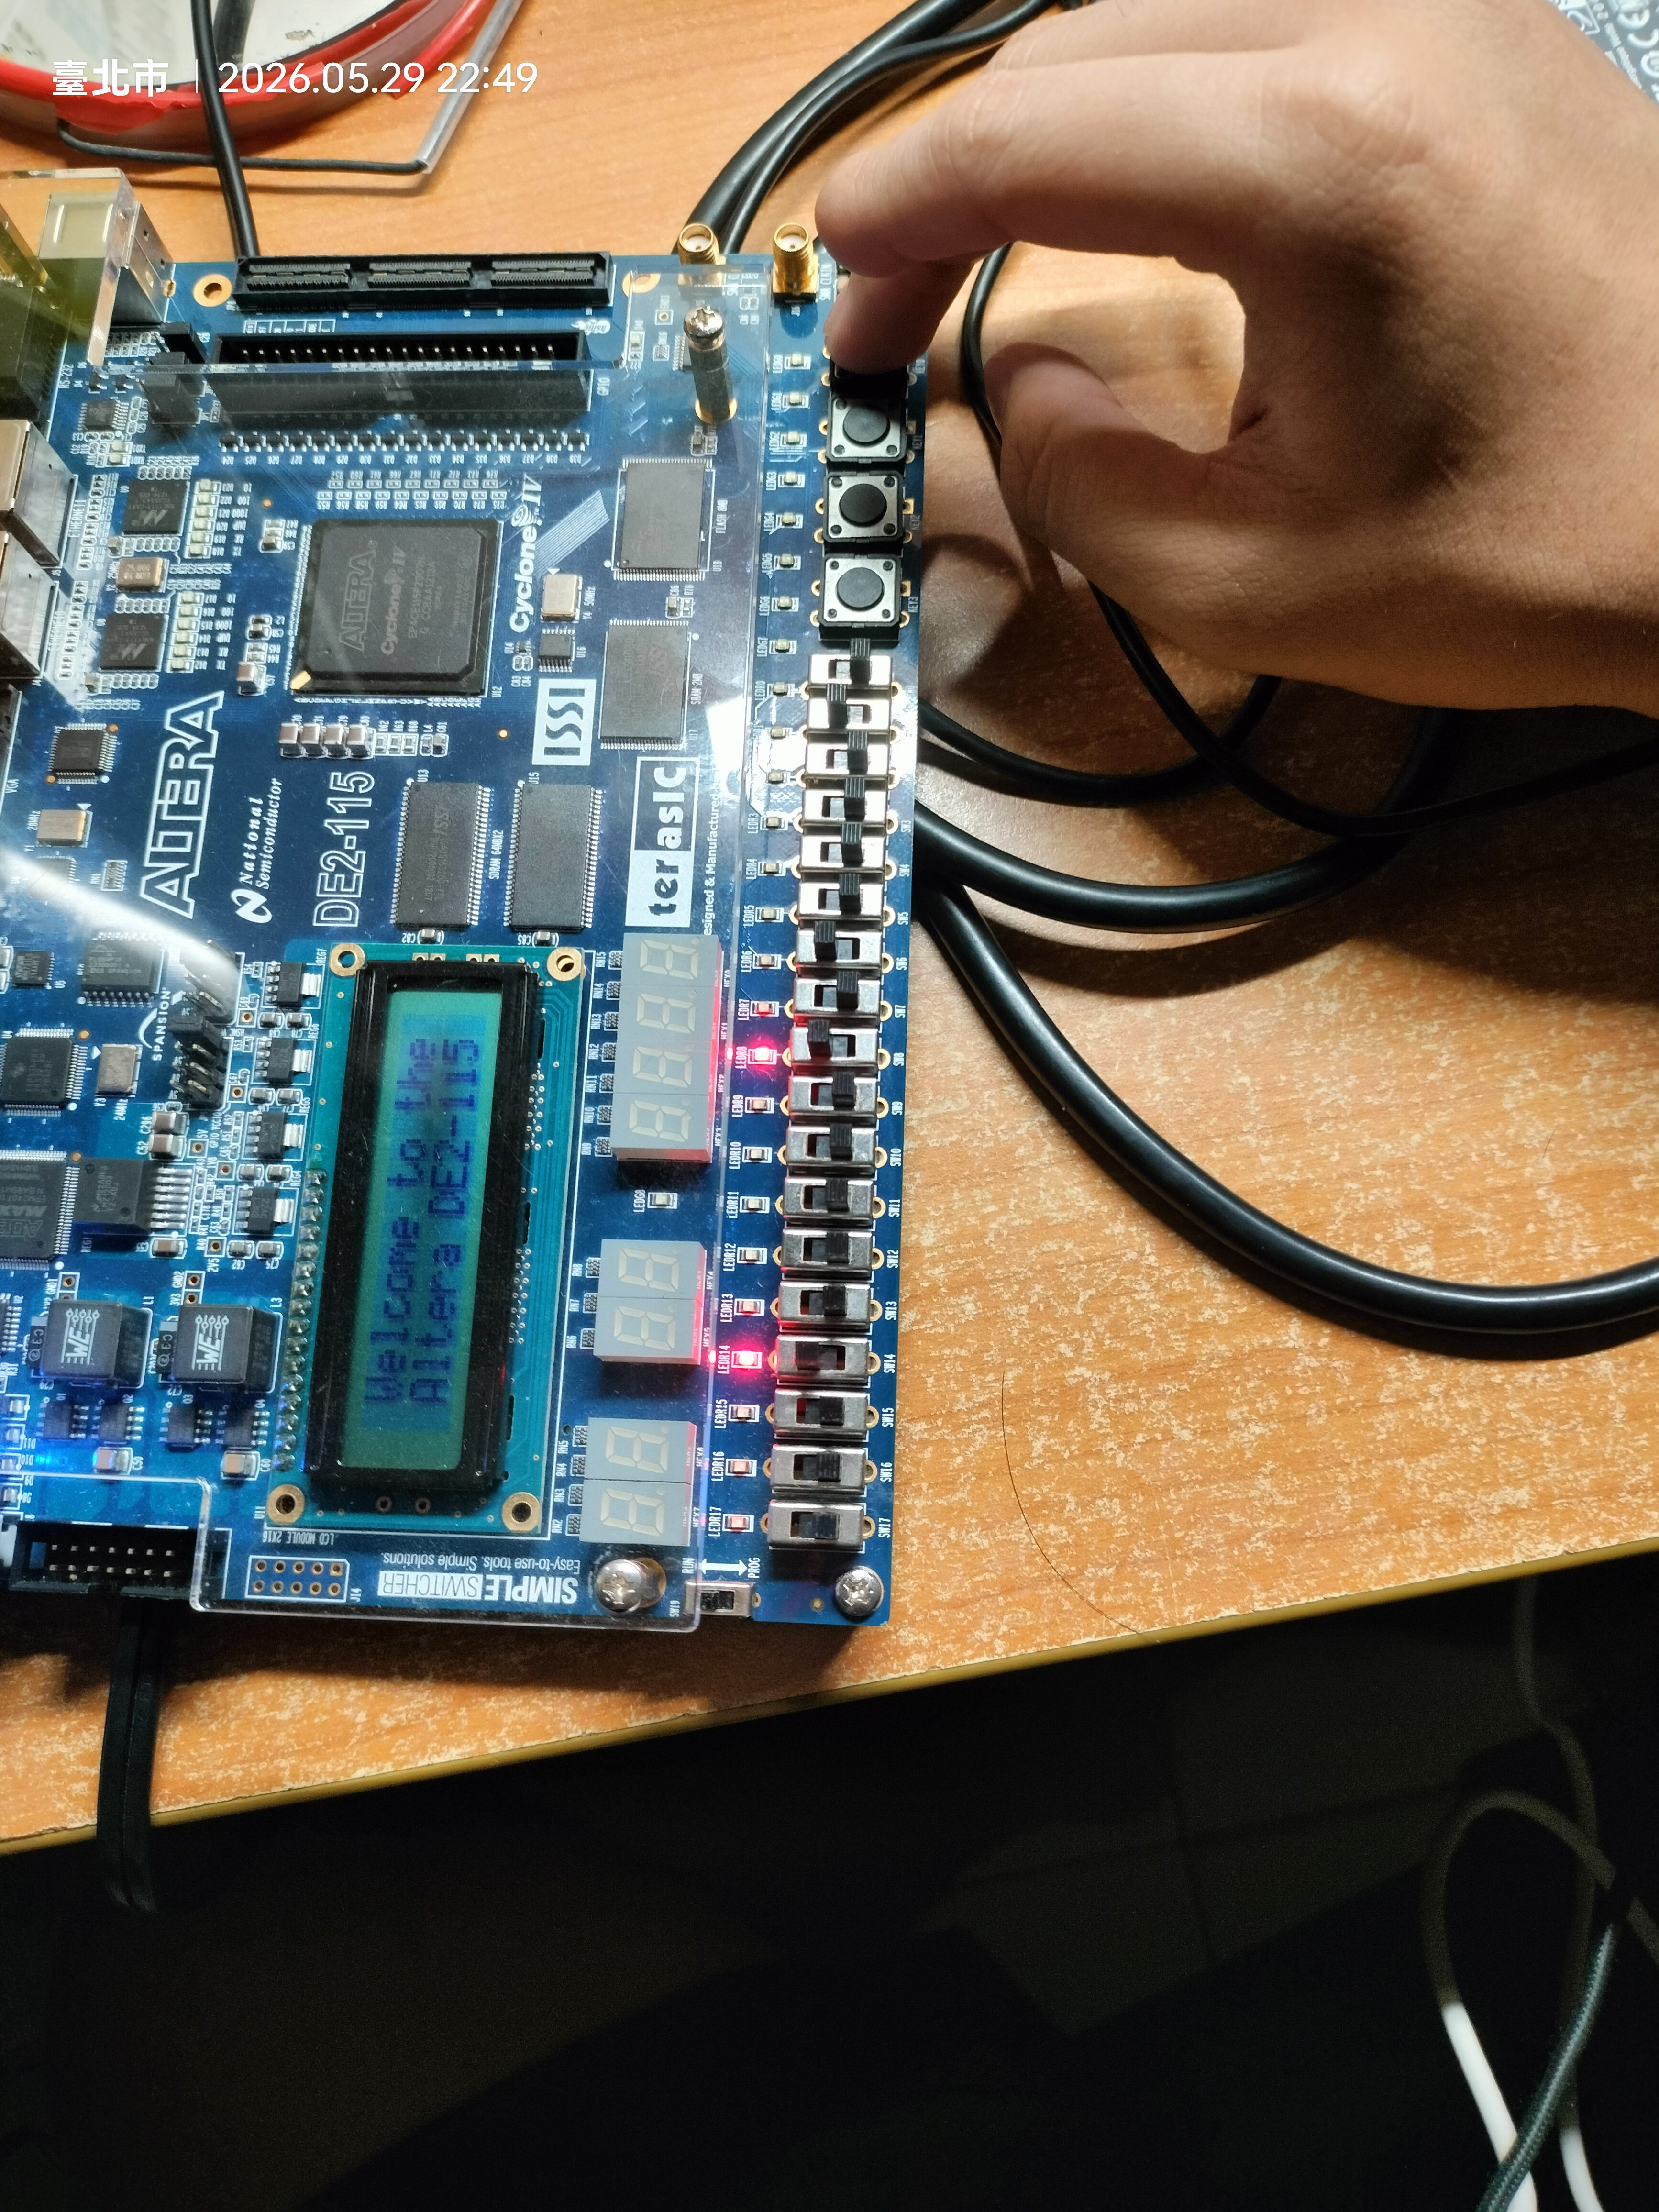
\includegraphics[width=0.65\textwidth]{../../photo/IMG20260529224937.jpg}
    \caption{第 9 次迭代後 S3 進入 S4（\texttt{count = 8}）：FSM 凍結，運算完成。}
\end{figure}

\begin{figure}[H]
    \centering
    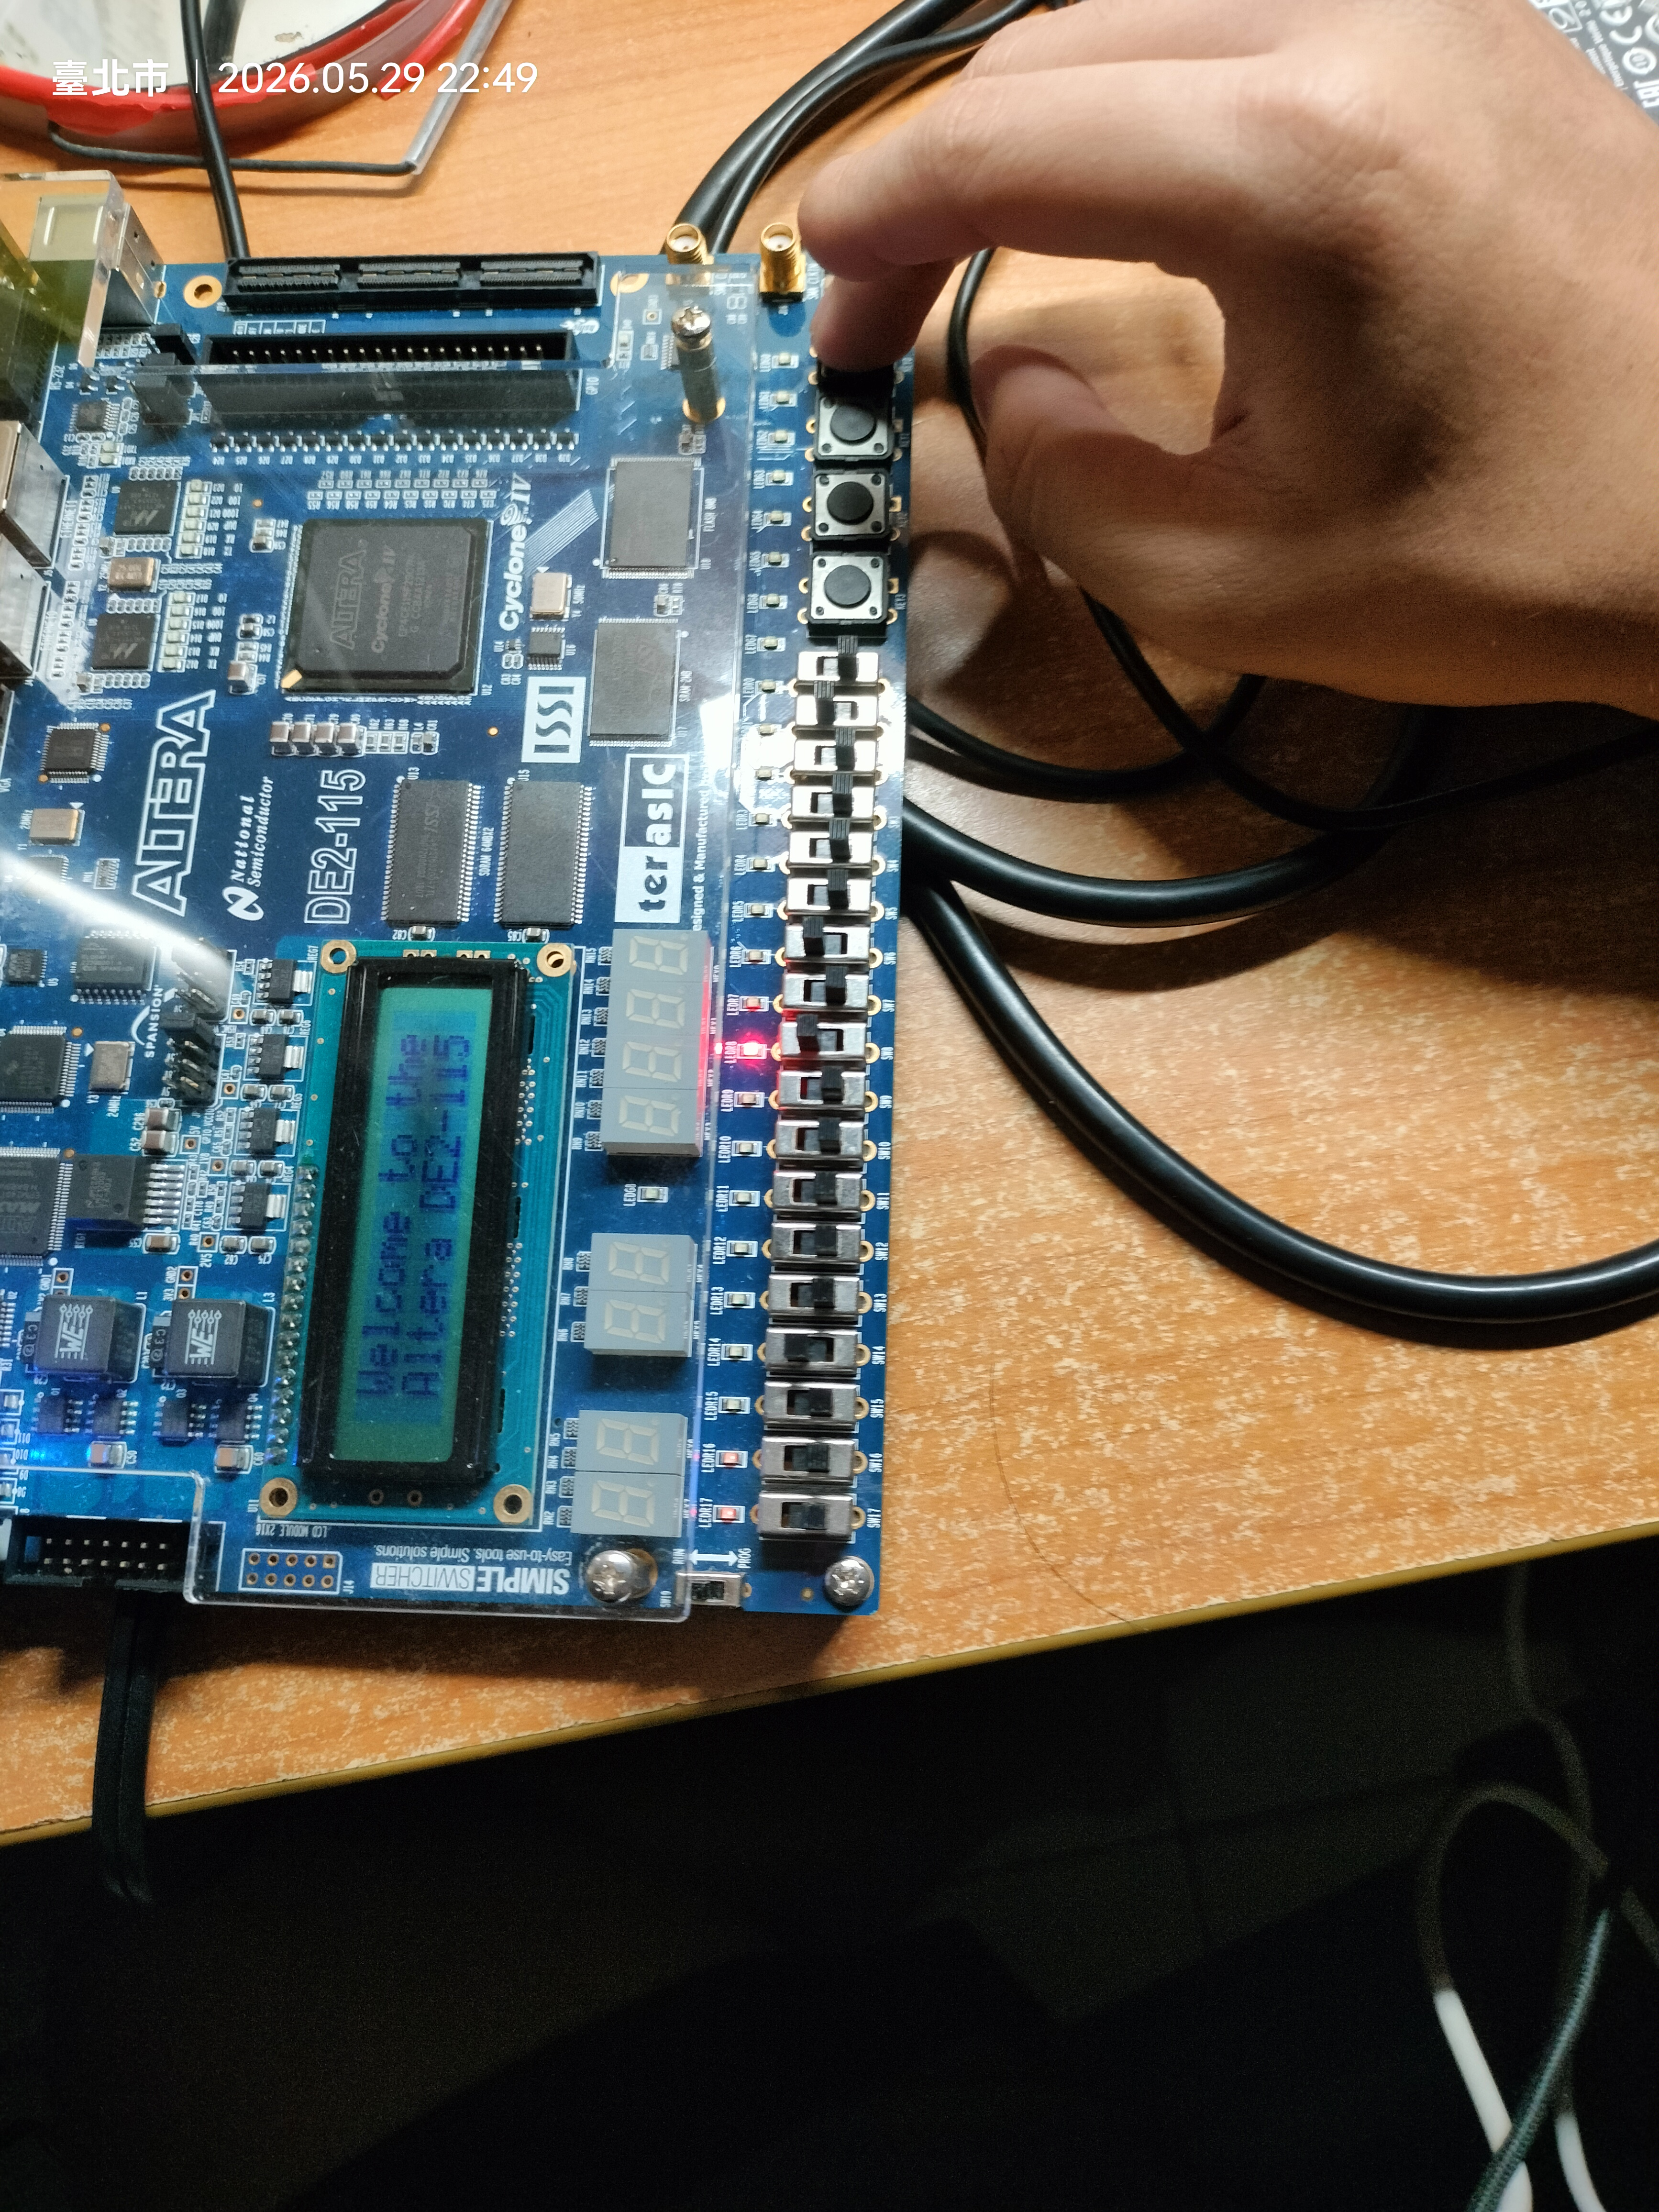
\includegraphics[width=0.65\textwidth]{../../photo/IMG20260529224939.jpg}
    \caption{S4 完成狀態（一）：HEX1:HEX0 顯示最終商數，HEX3:HEX2 顯示最終餘數（十六進位格式）。}
\end{figure}

\begin{figure}[H]
    \centering
    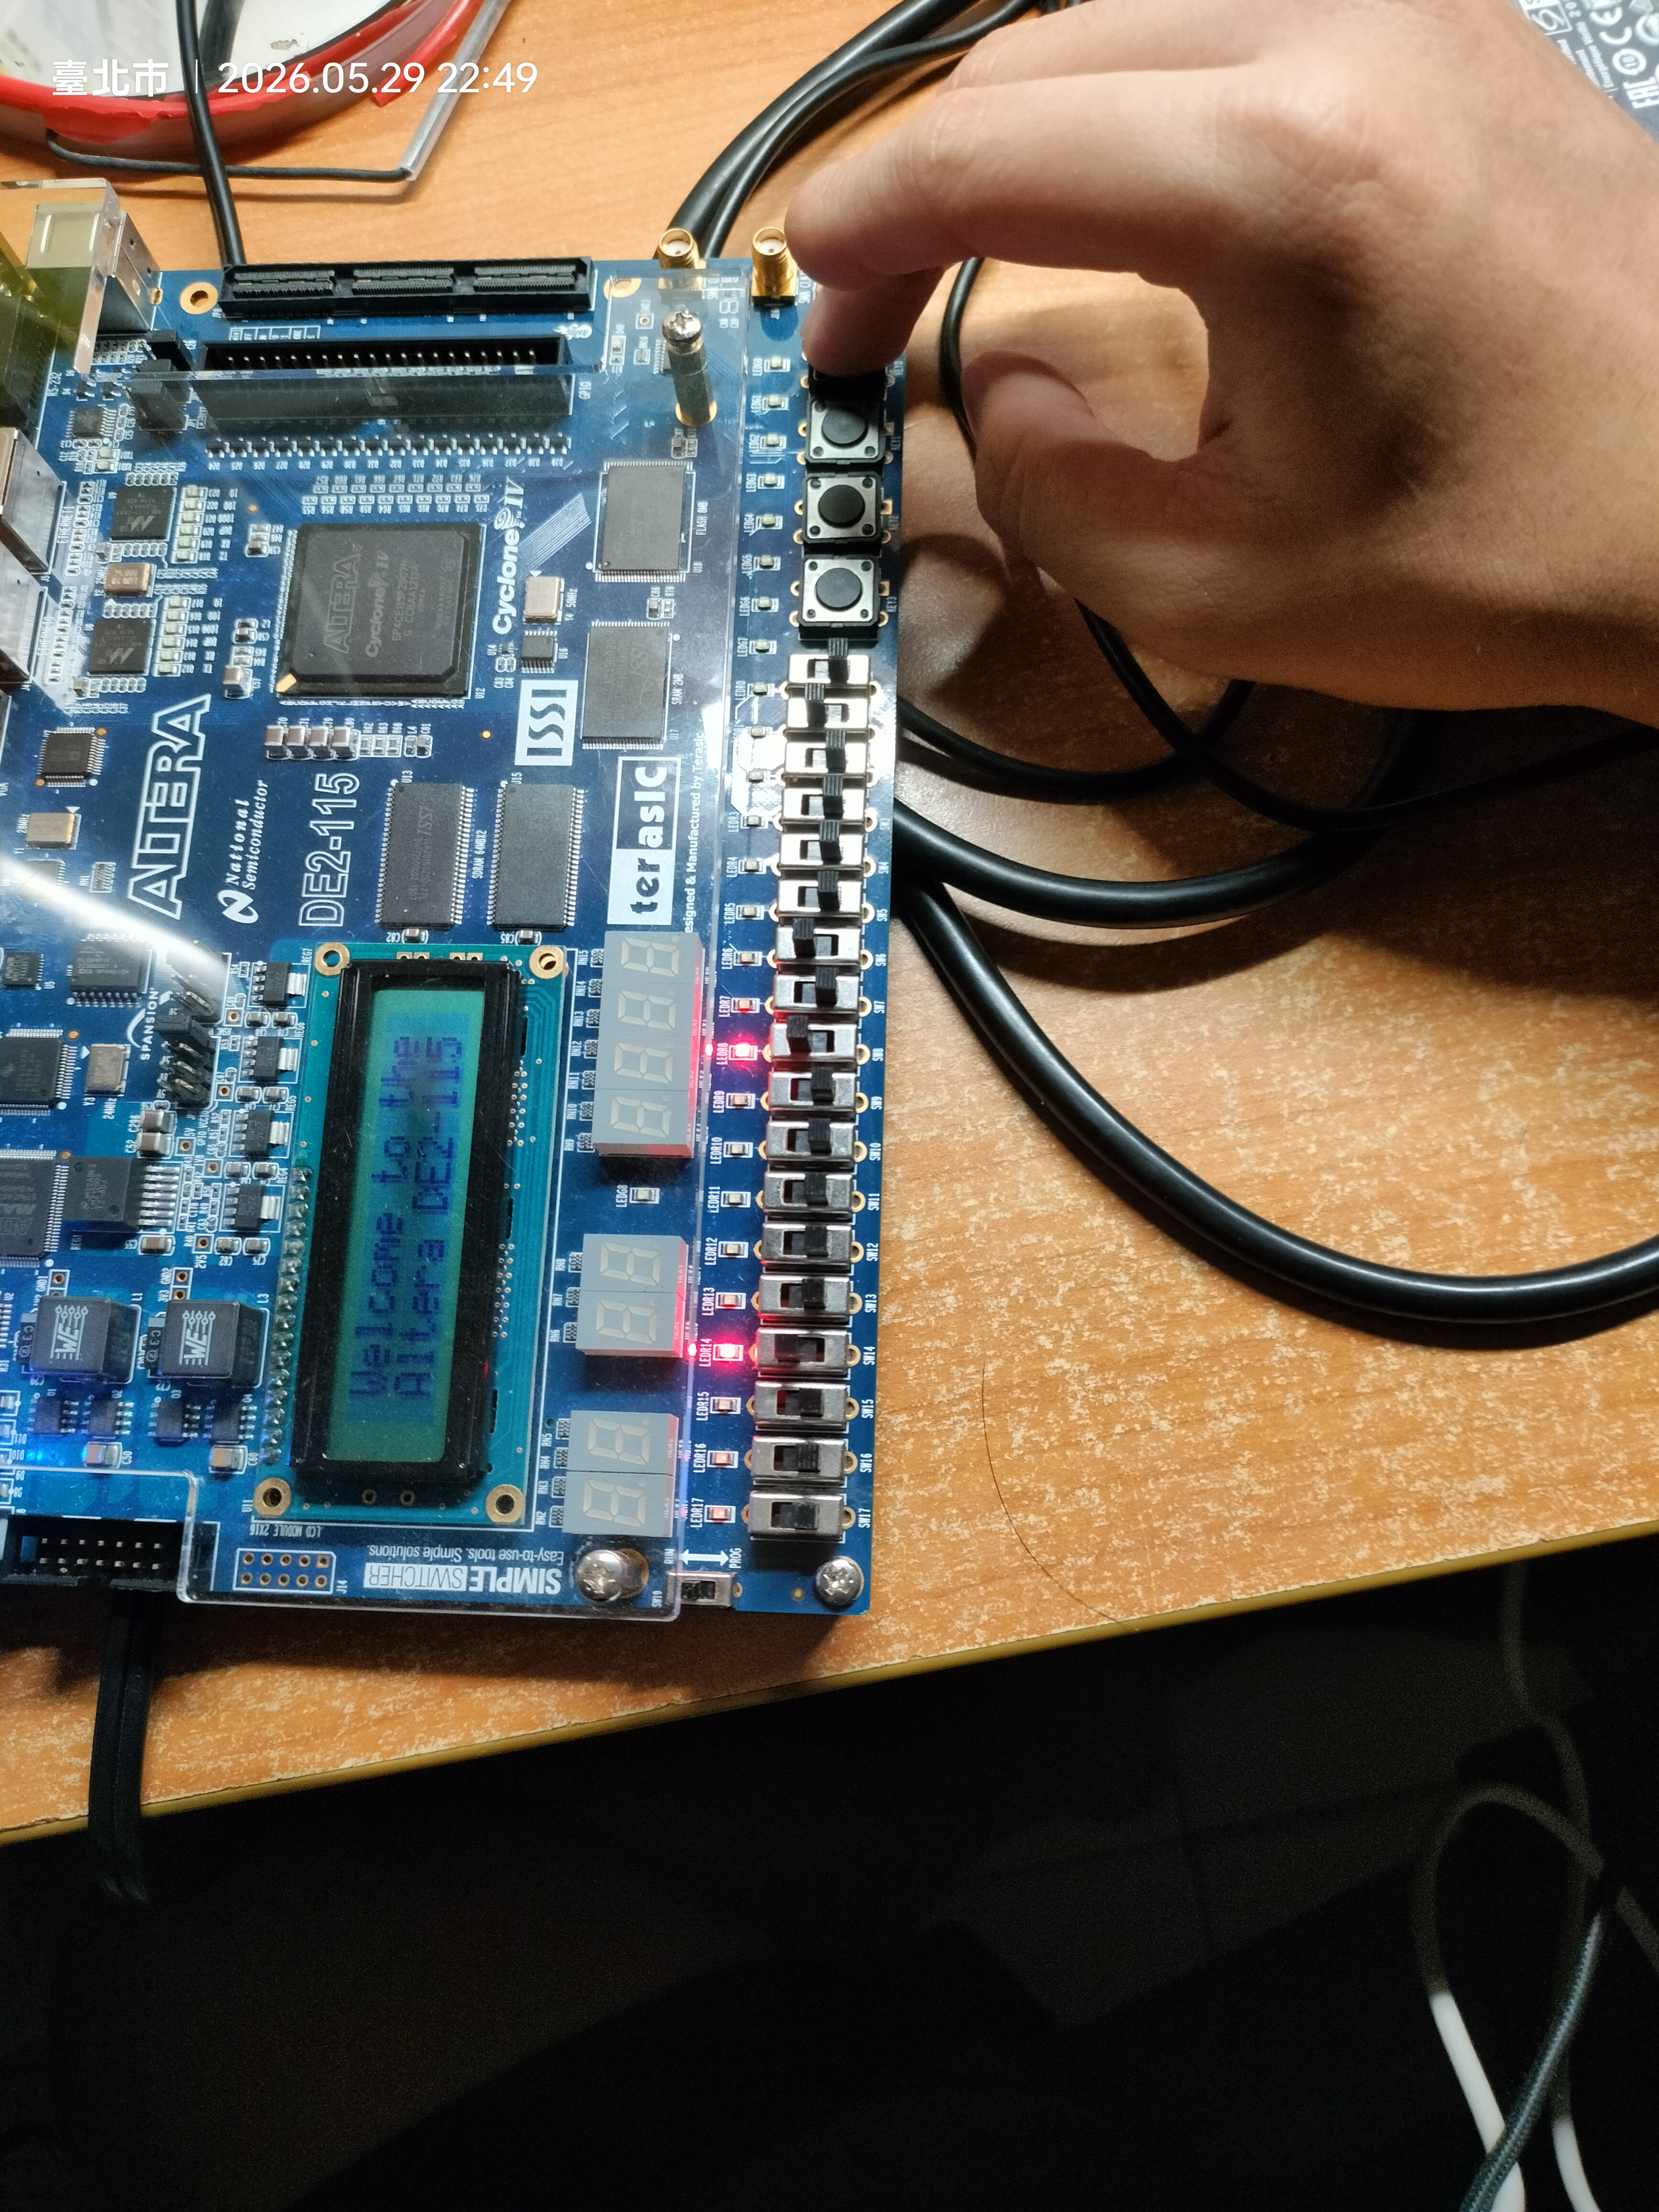
\includegraphics[width=0.65\textwidth]{../../photo/IMG20260529224941.jpg}
    \caption{S4 完成狀態（二）：整體開發板正面照，確認七段顯示器顯示最終計算結果。}
\end{figure}

\begin{figure}[H]
    \centering
    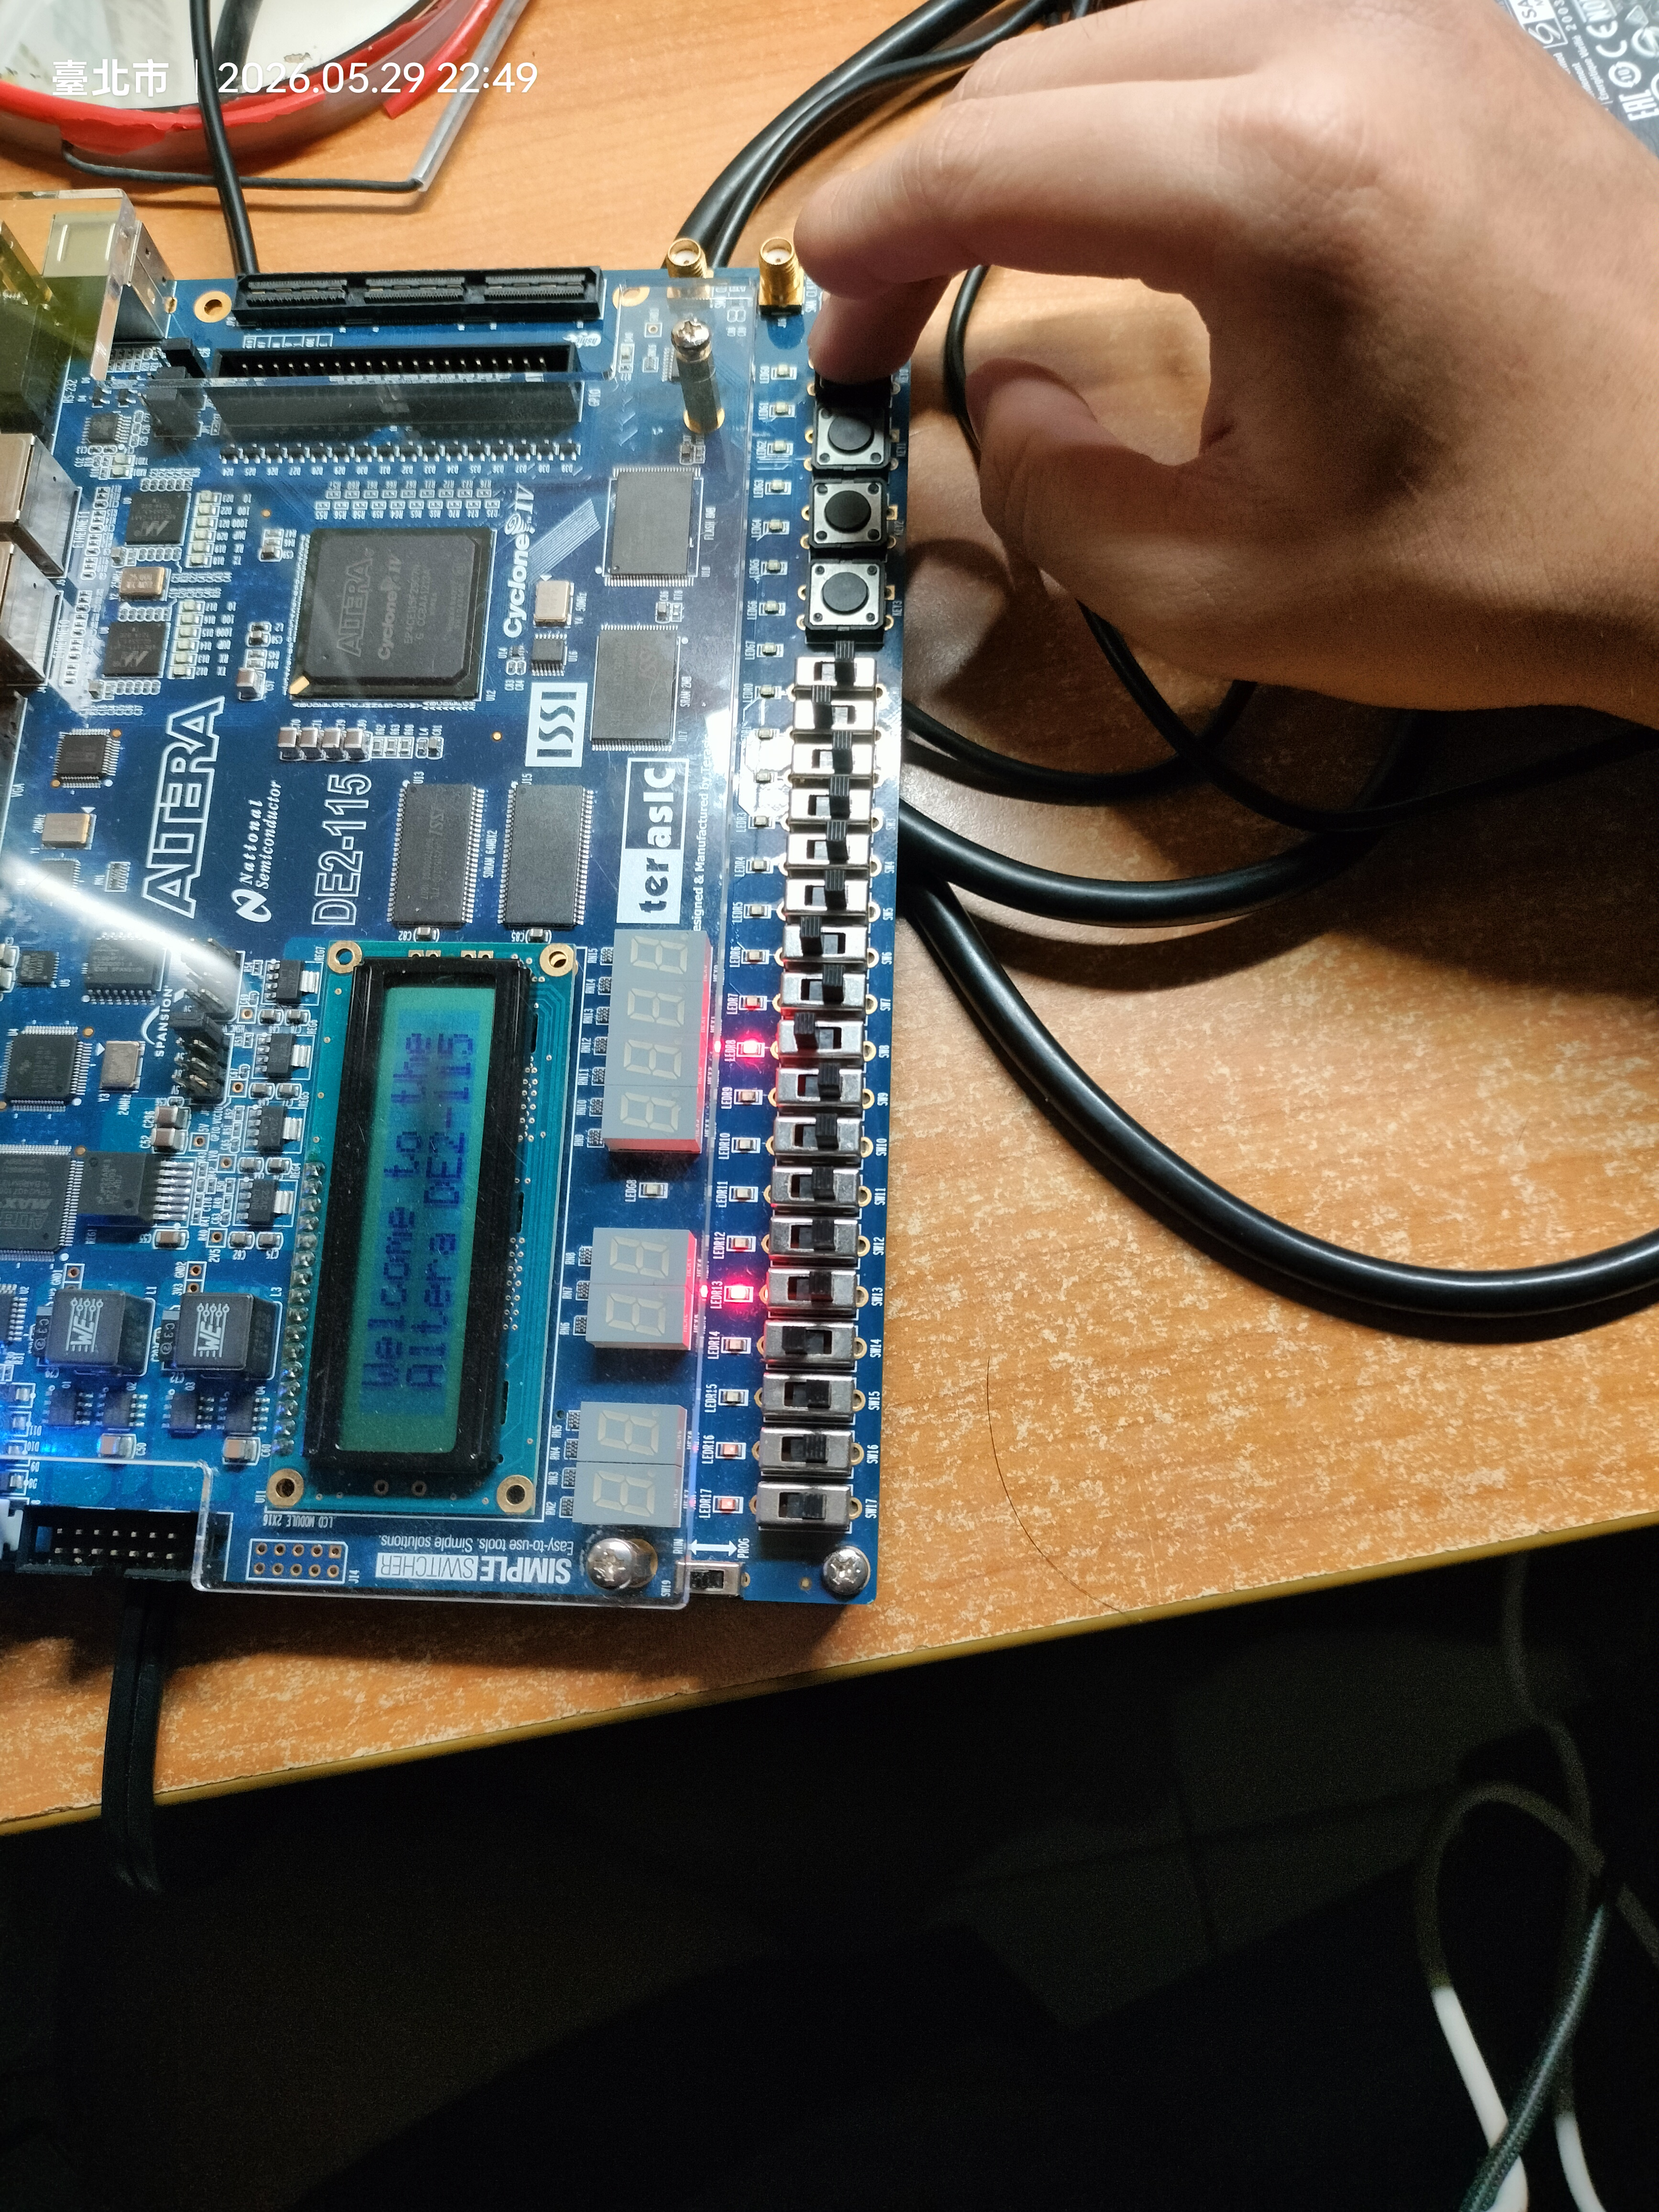
\includegraphics[width=0.65\textwidth]{../../photo/IMG20260529224942.jpg}
    \caption{S4 完成狀態（三）：近距離確認四個七段顯示器上的數值正確無誤。}
\end{figure}

\begin{figure}[H]
    \centering
    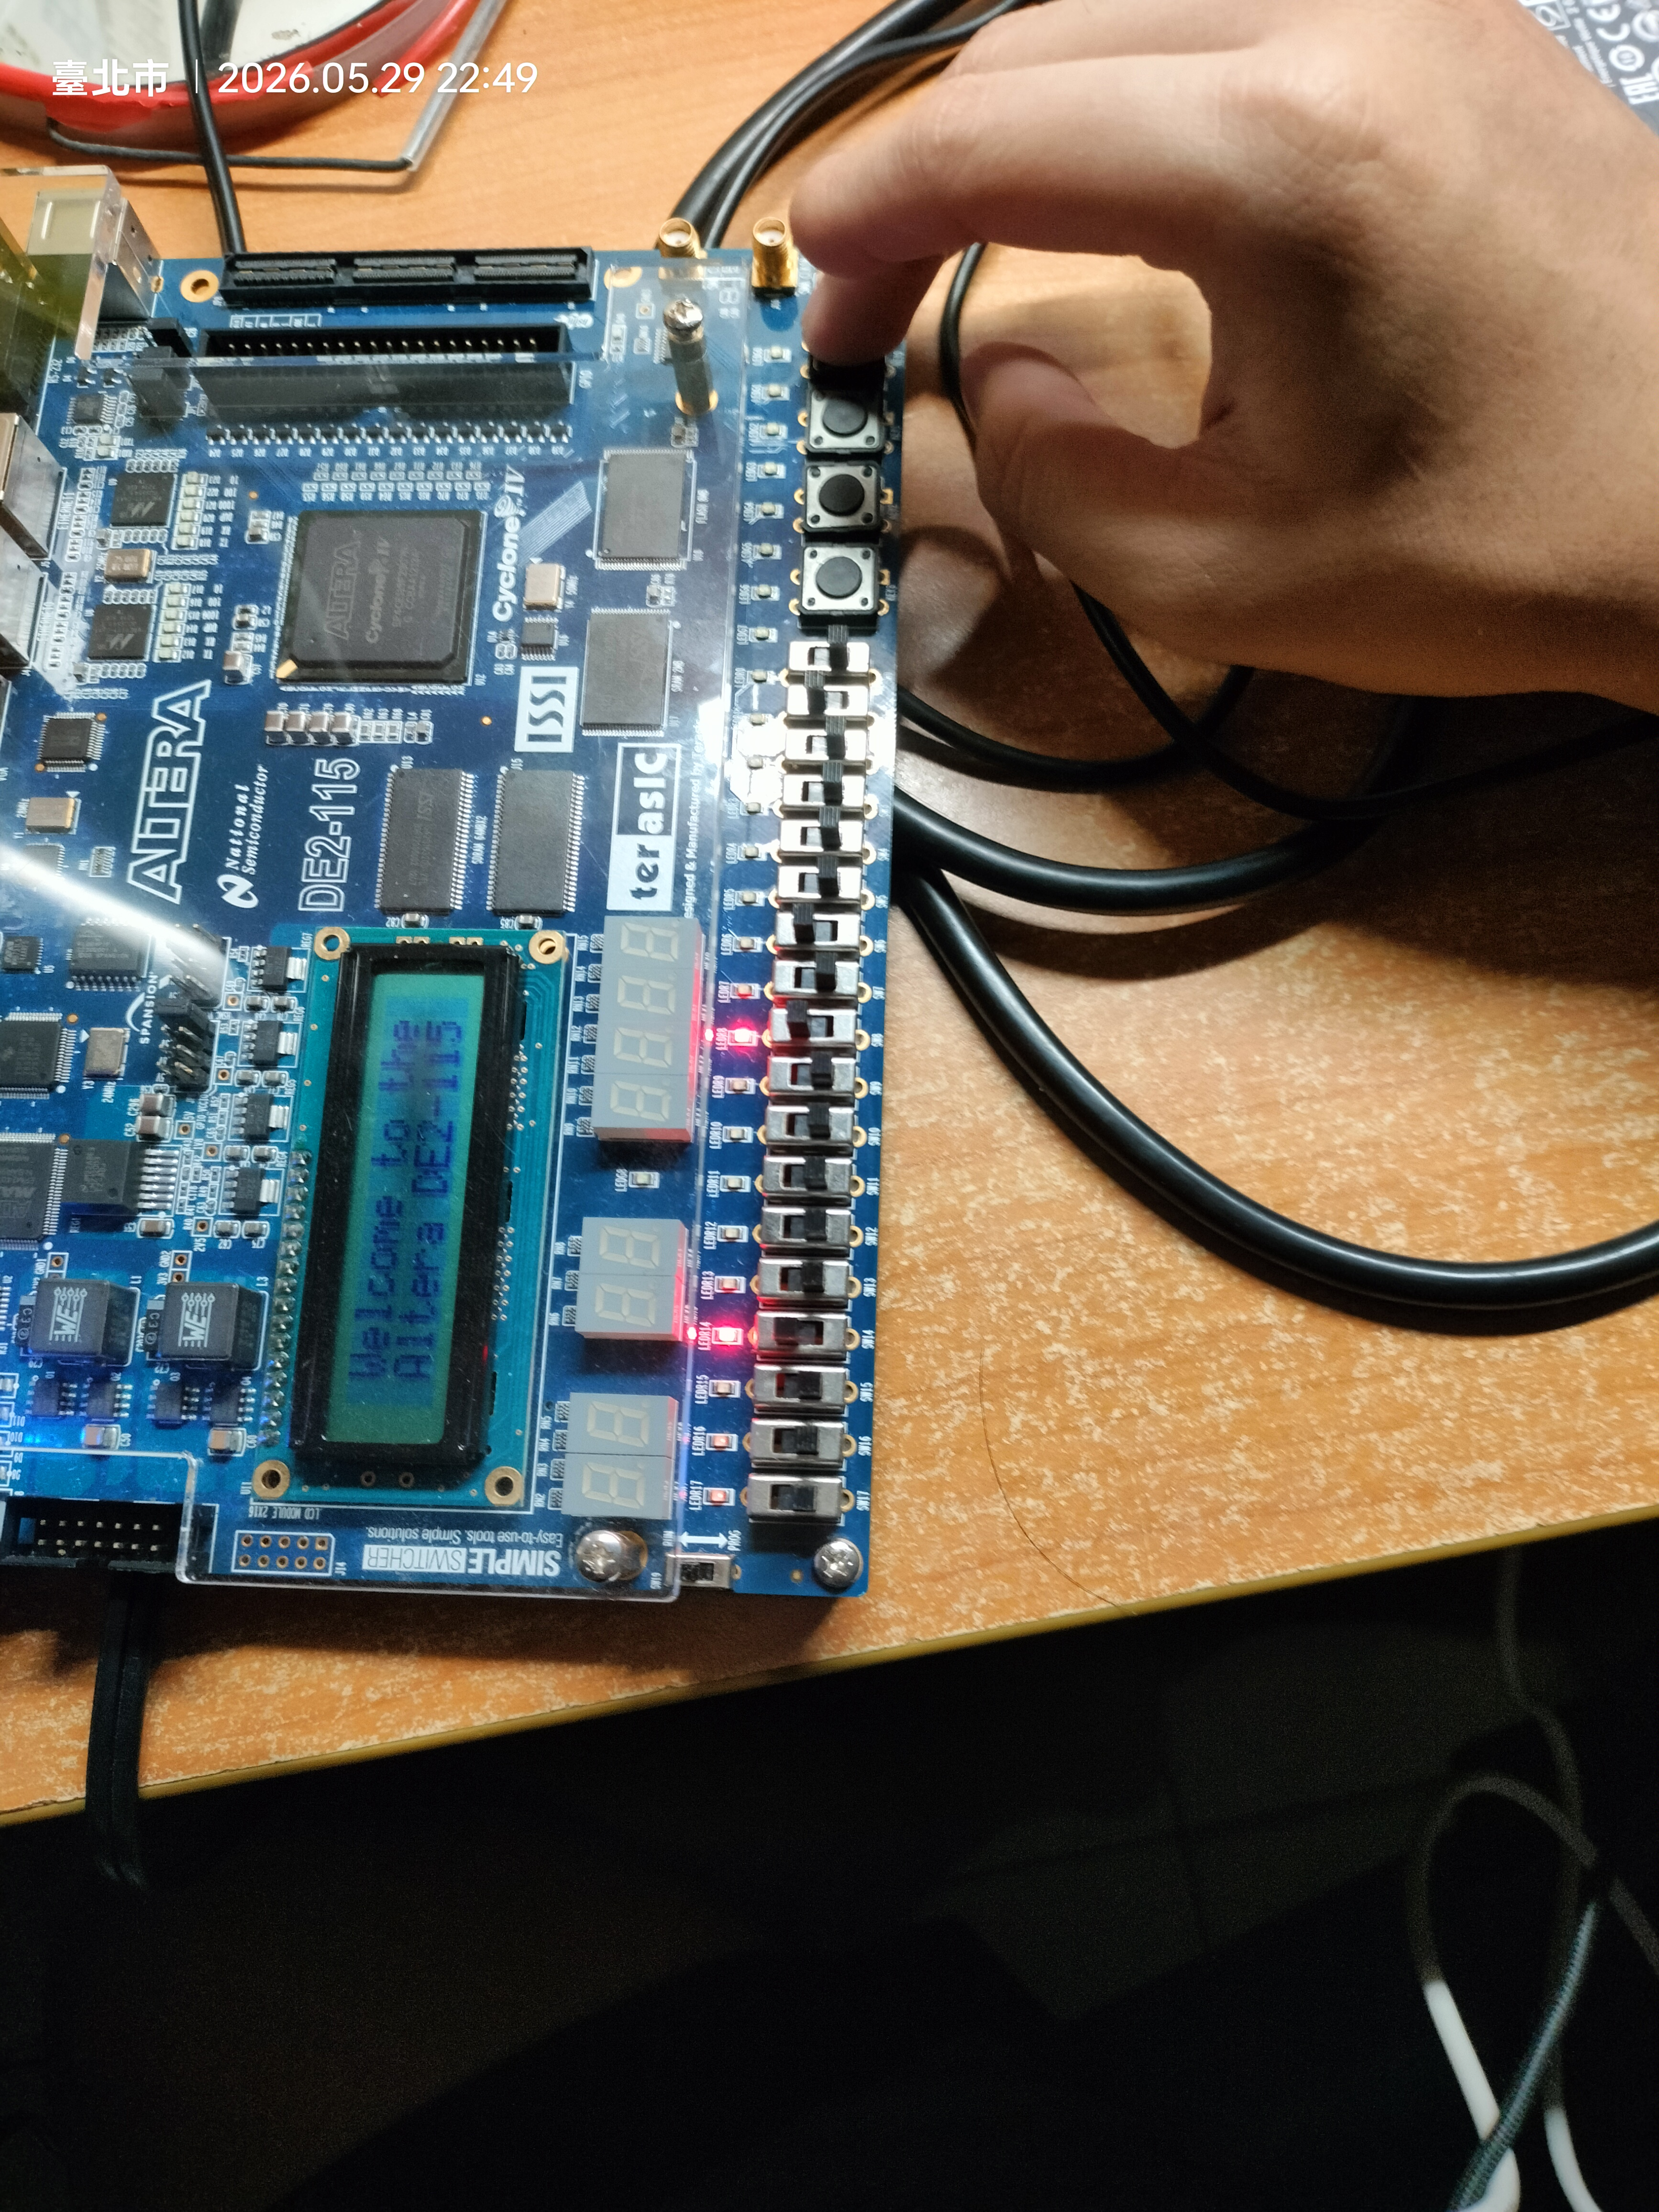
\includegraphics[width=0.65\textwidth]{../../photo/IMG20260529224944.jpg}
    \caption{驗證另一組輸入：更換 SW 撥碼開關設定，確認除法器對不同輸入值的運算正確性。}
\end{figure}

\begin{figure}[H]
    \centering
    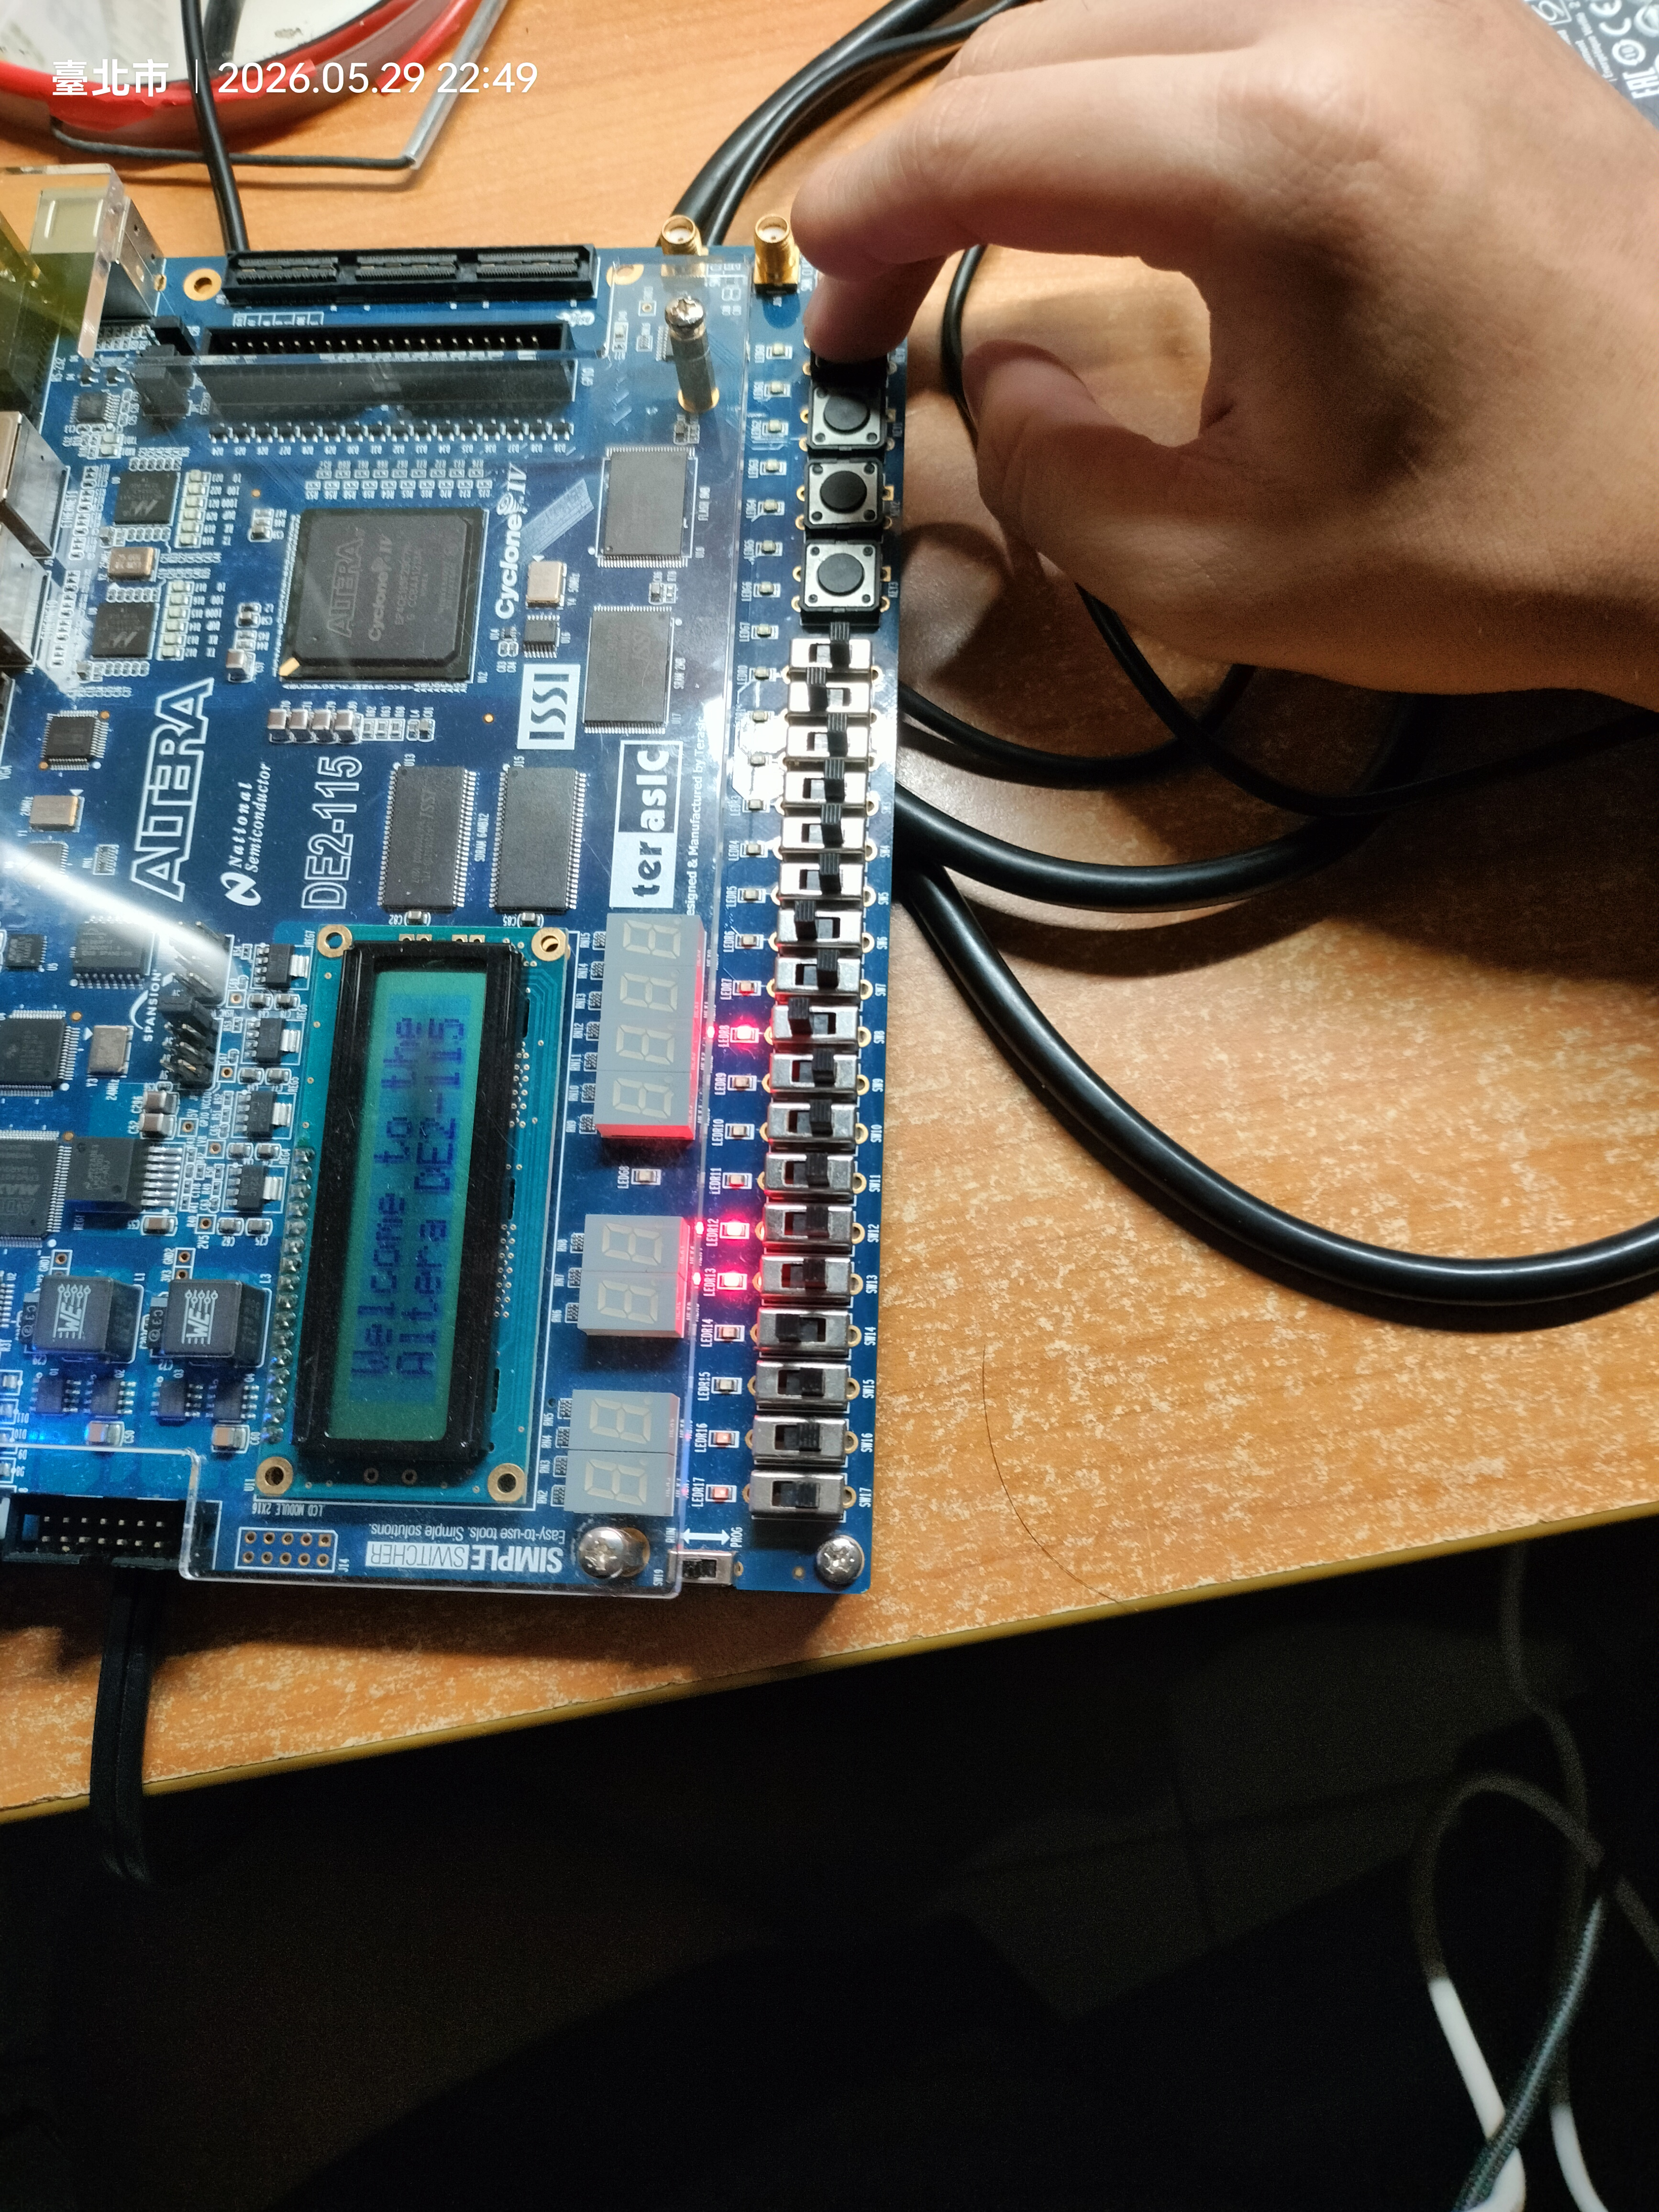
\includegraphics[width=0.65\textwidth]{../../photo/IMG20260529224946.jpg}
    \caption{重新 Reset 後再次運算（一）：SW[16] 撥高後，FSM 回到 Start 狀態，系統就緒。}
\end{figure}

\begin{figure}[H]
    \centering
    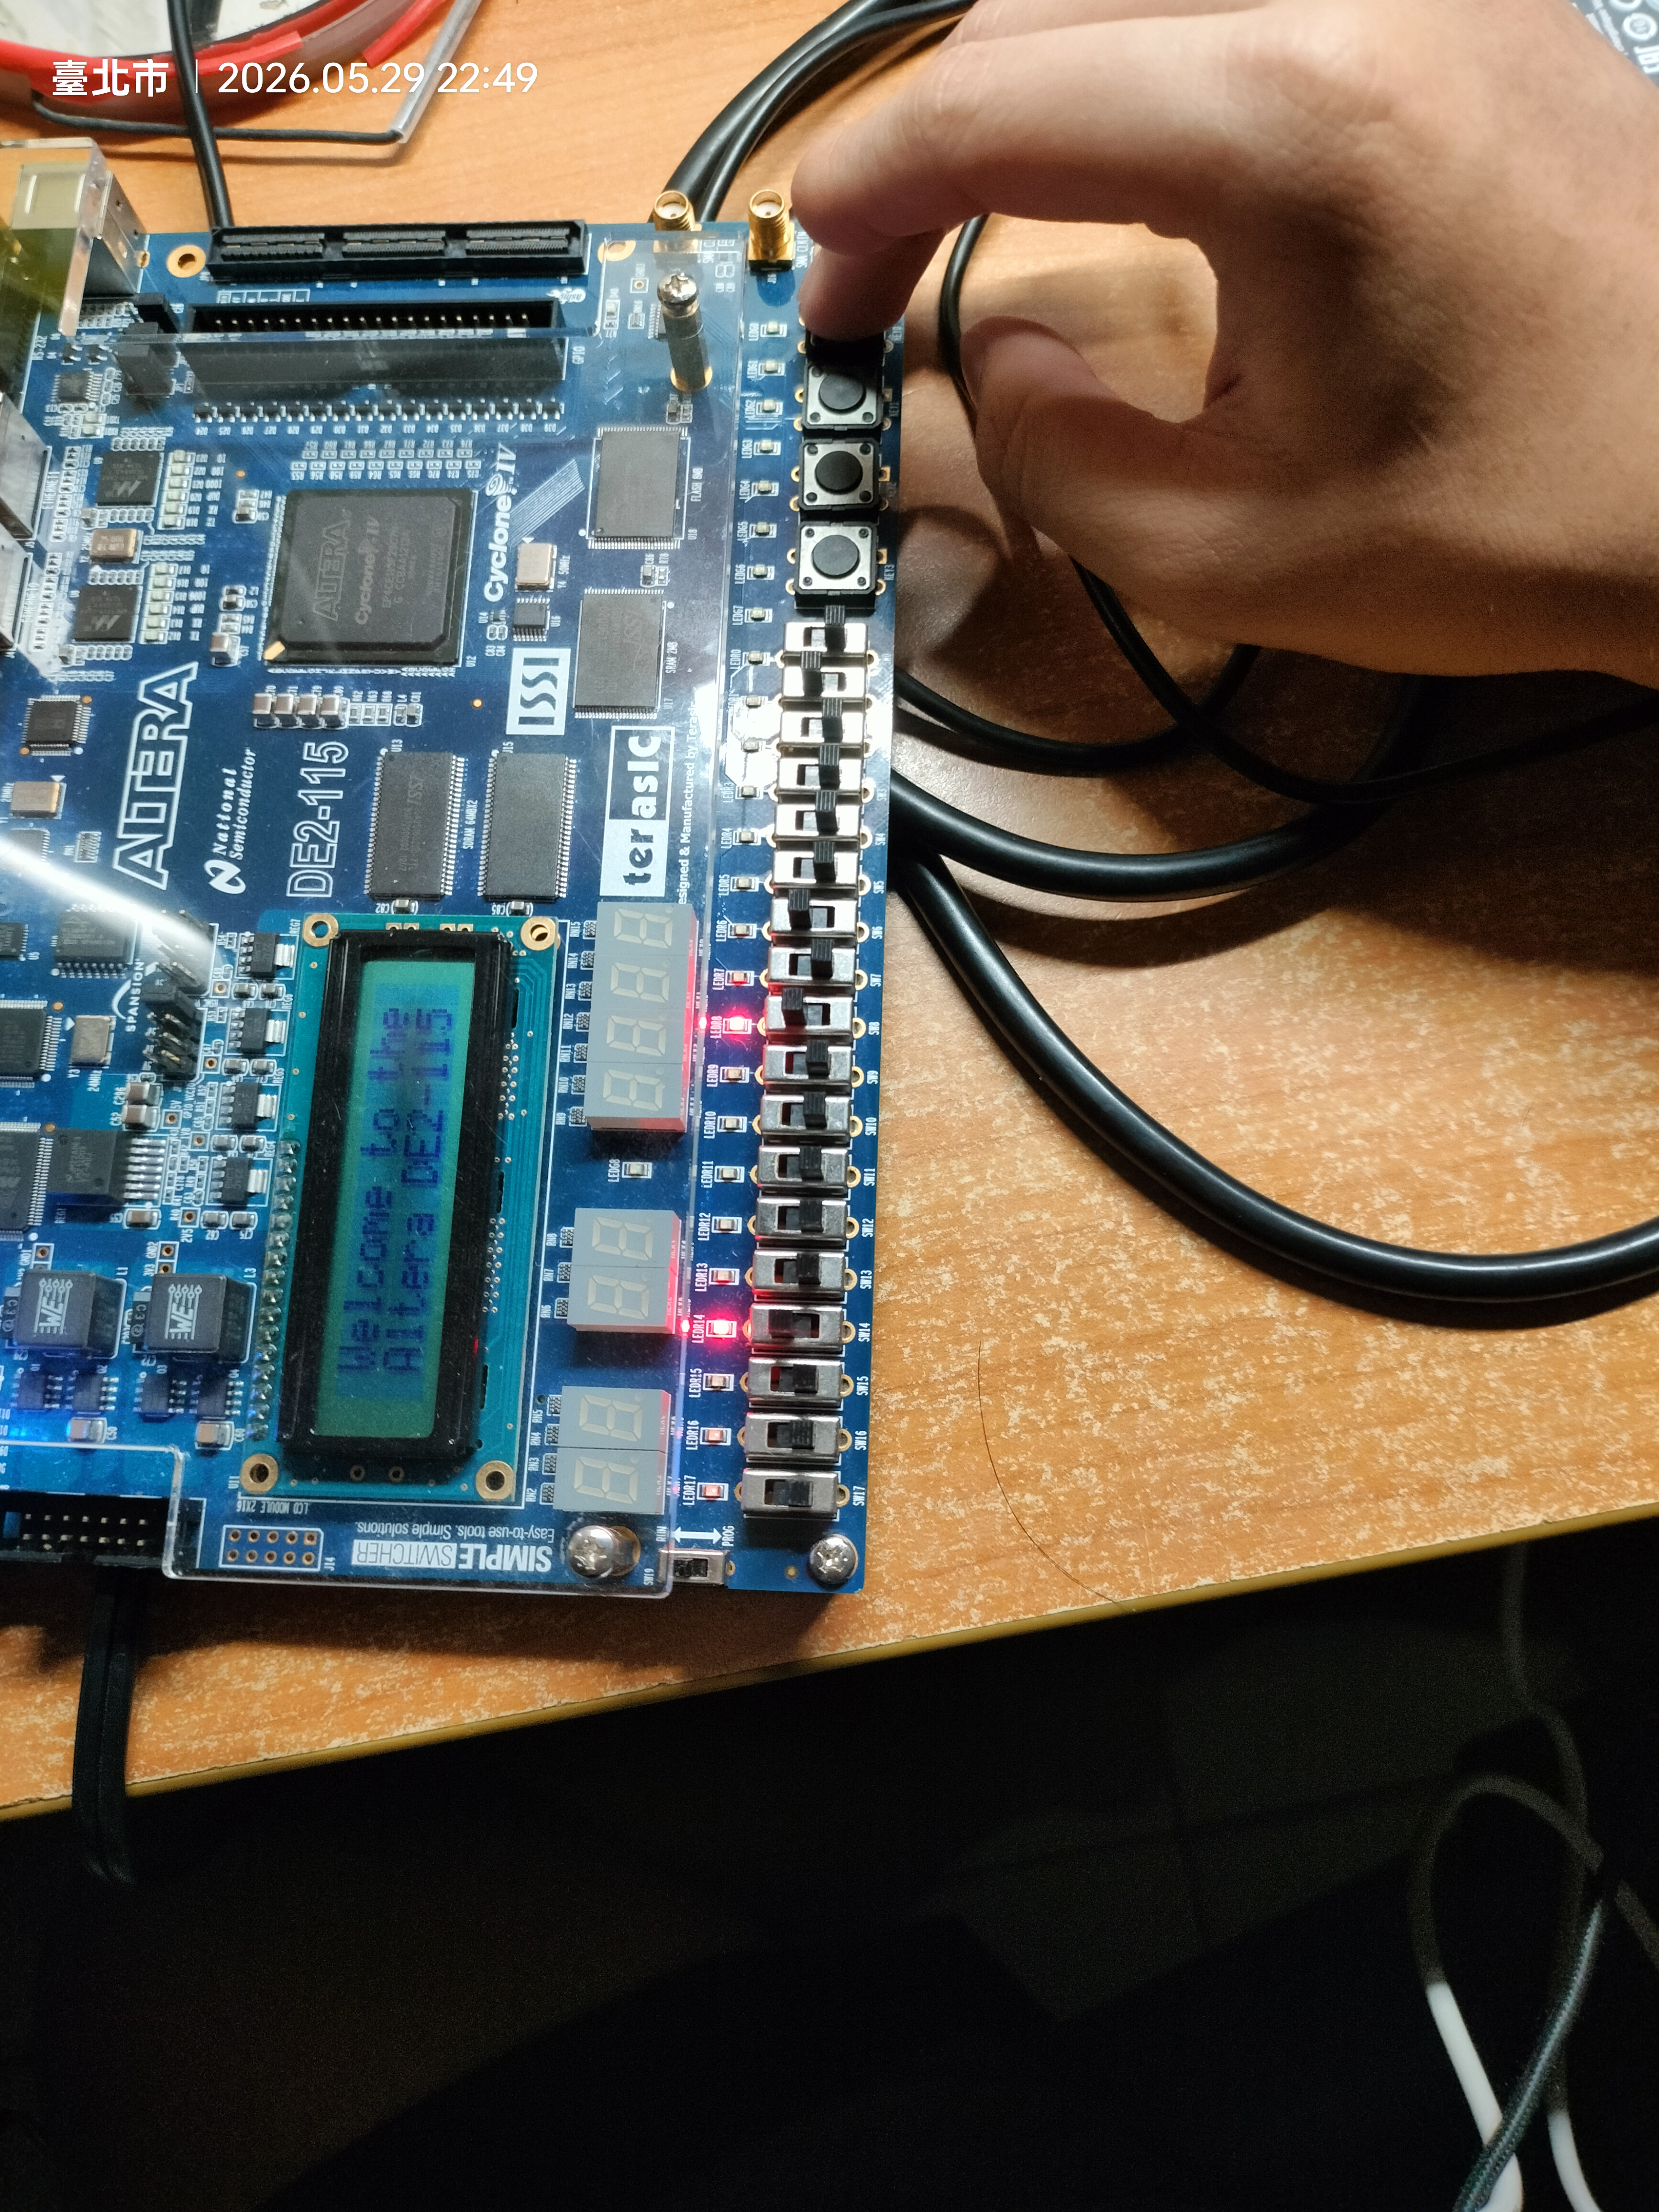
\includegraphics[width=0.65\textwidth]{../../photo/IMG20260529224948.jpg}
    \caption{重新 Reset 後再次運算（二）：設定新的被除數與除數，逐步驗證第二組測試案例。}
\end{figure}

\begin{figure}[H]
    \centering
    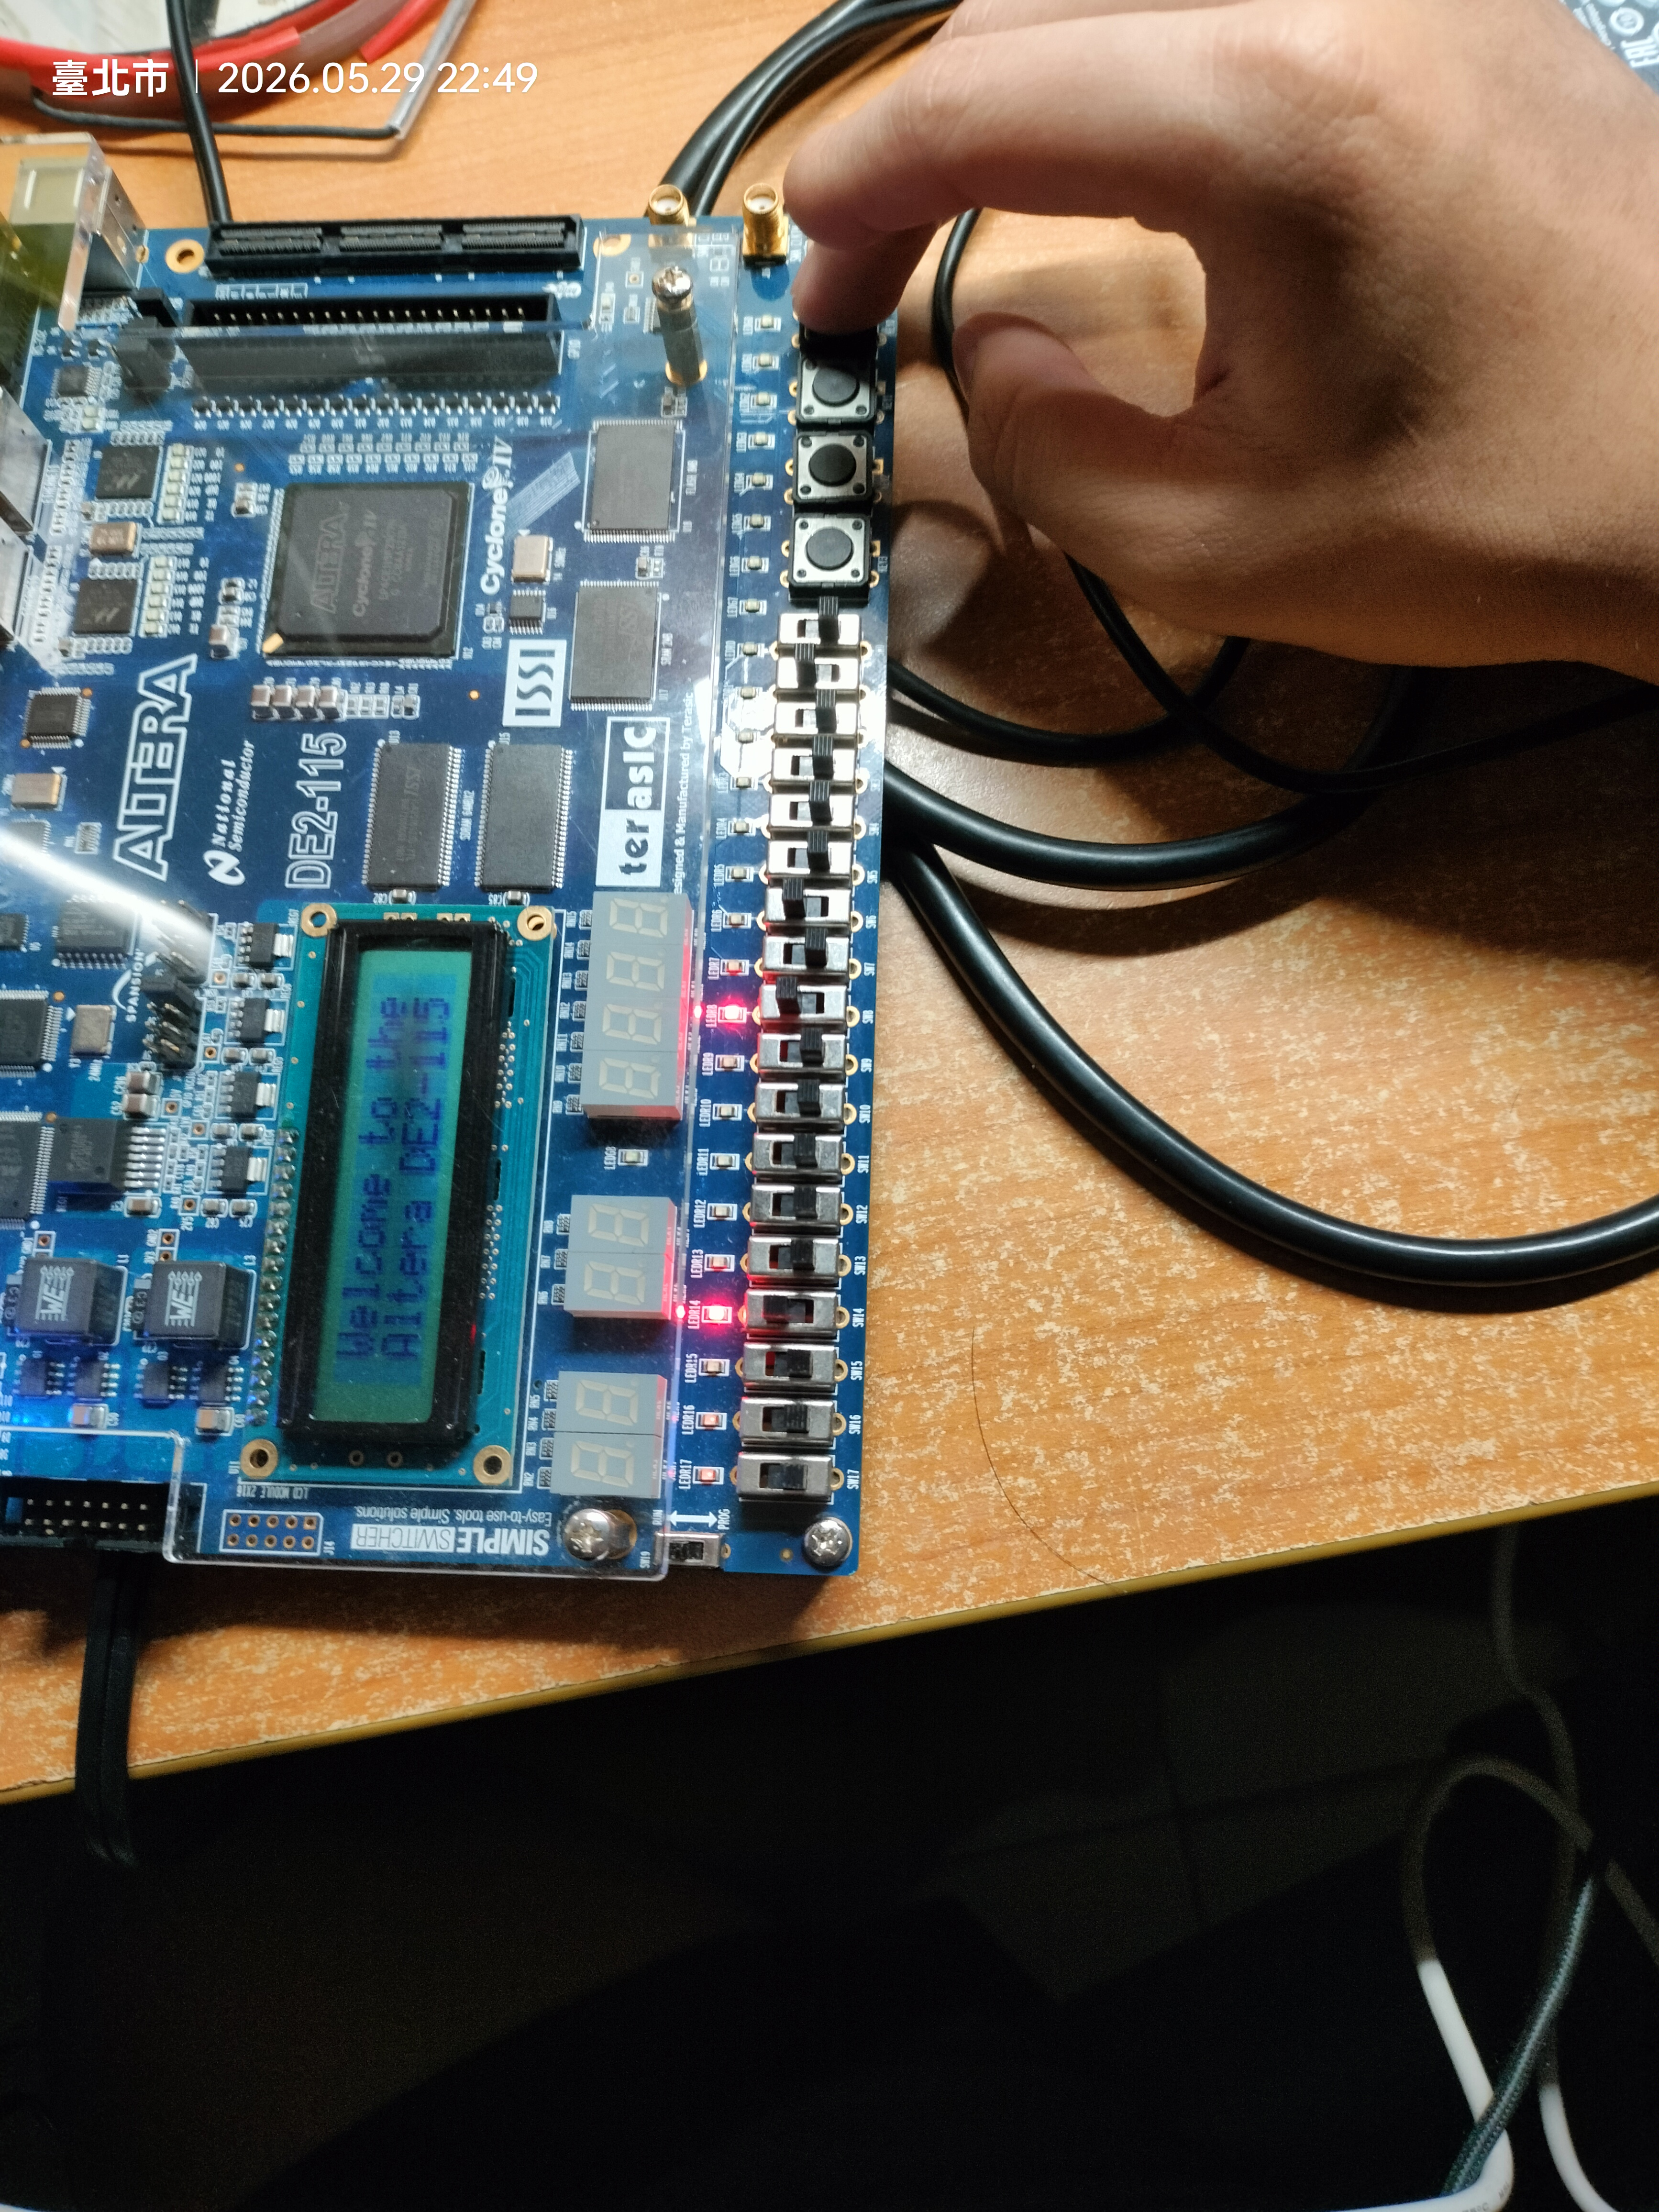
\includegraphics[width=0.65\textwidth]{../../photo/IMG20260529224950.jpg}
    \caption{第二組測試的中間迭代過程：LED 顯示不同輸入下各步驟的暫存器狀態。}
\end{figure}

\begin{figure}[H]
    \centering
    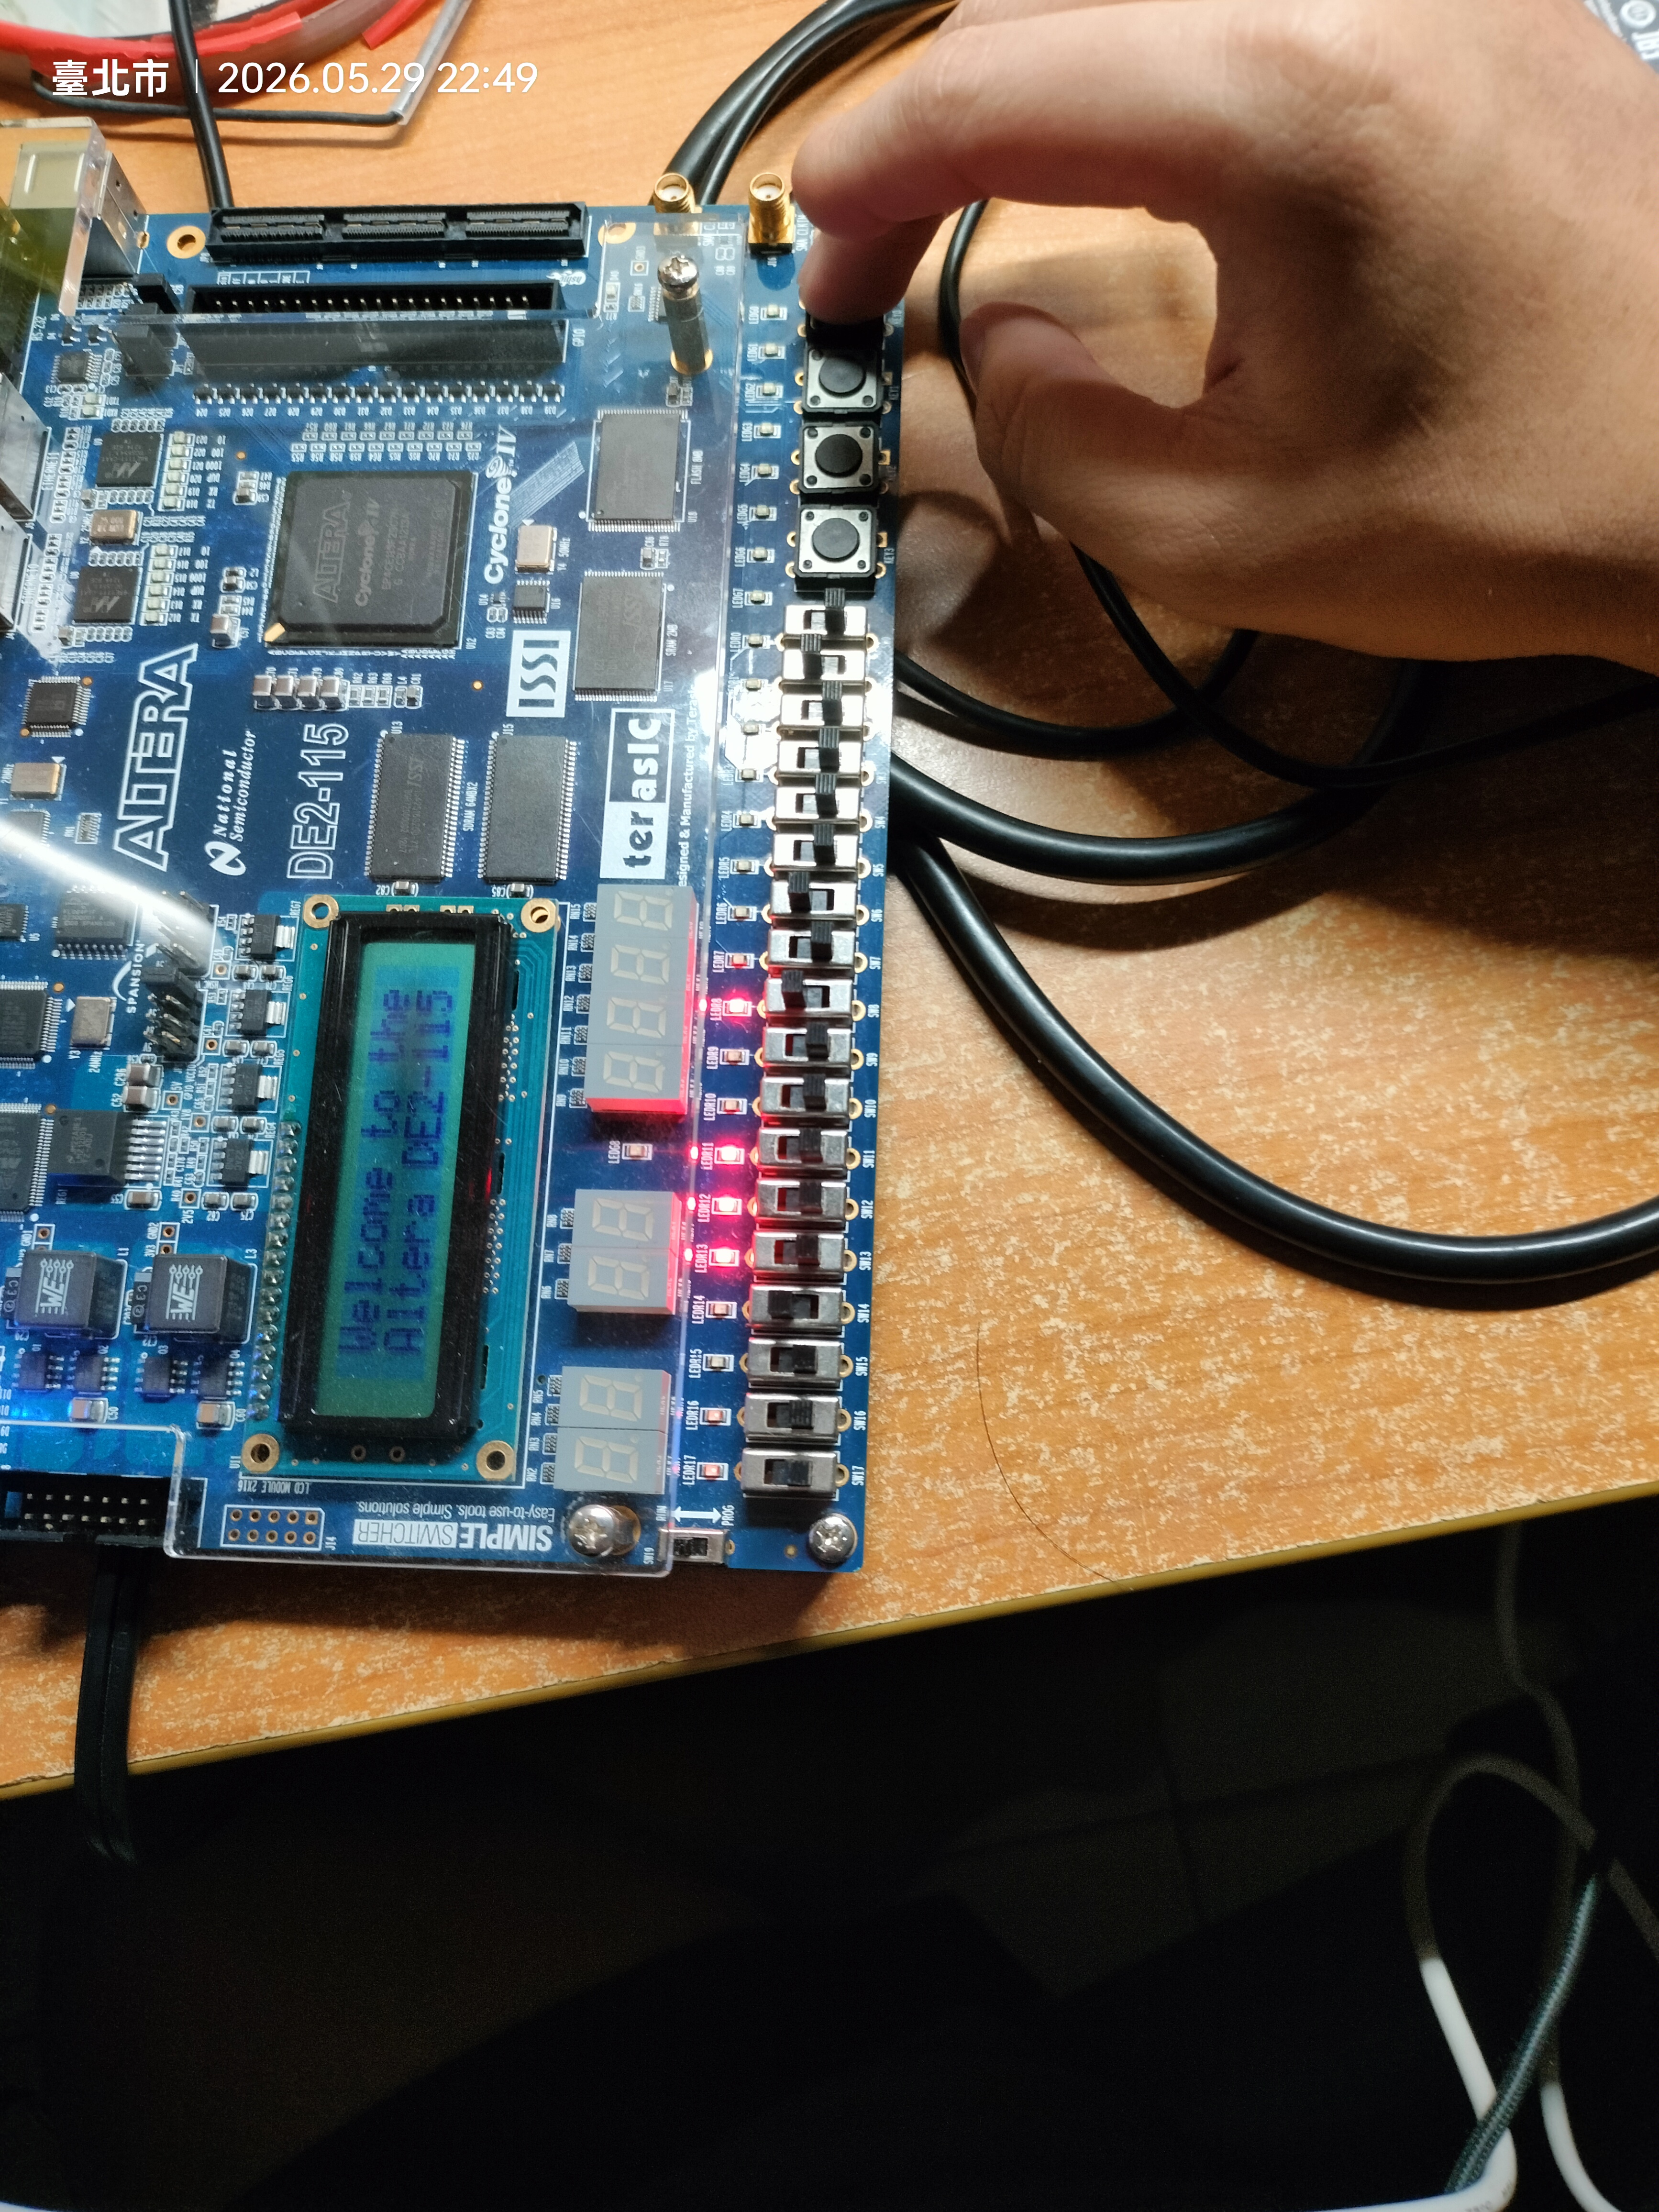
\includegraphics[width=0.65\textwidth]{../../photo/IMG20260529224952.jpg}
    \caption{第二組測試的 S4 結果（一）：七段顯示器顯示新輸入的最終商與餘數。}
\end{figure}

\begin{figure}[H]
    \centering
    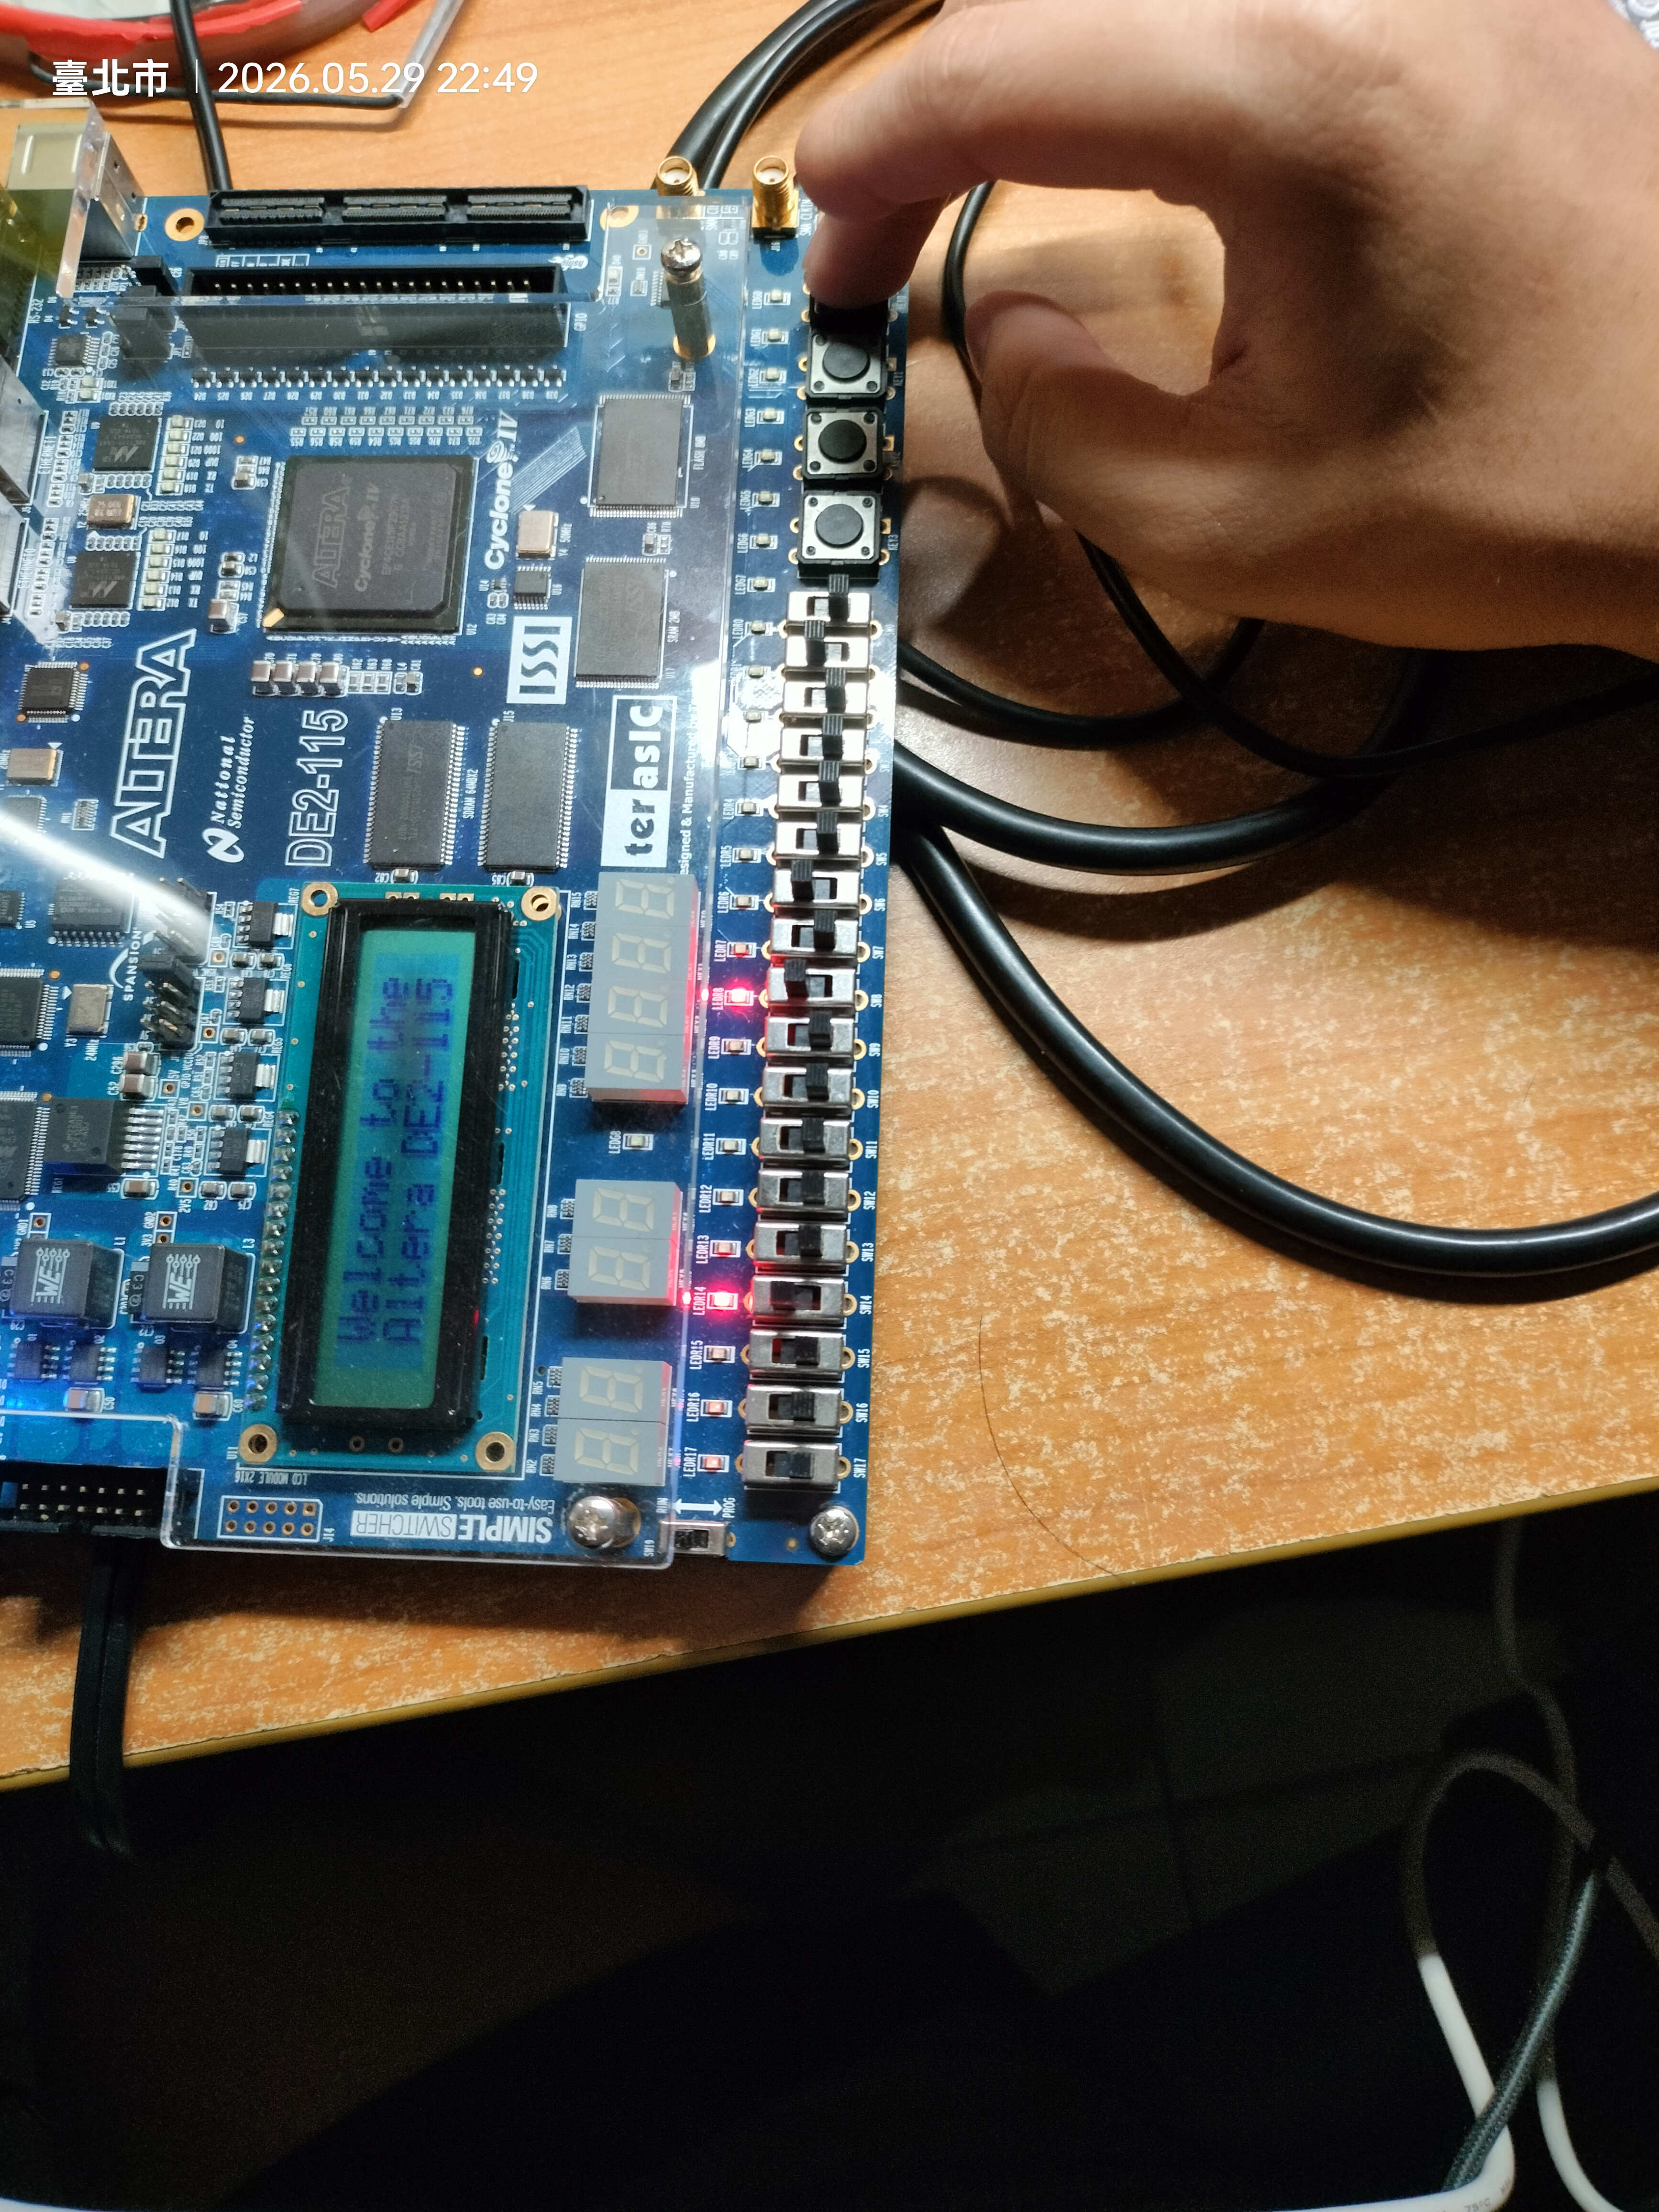
\includegraphics[width=0.65\textwidth]{../../photo/IMG20260529224953.jpg}
    \caption{第二組測試的 S4 結果（二）：完整板面照，確認 LED 與七段顯示器輸出一致。}
\end{figure}

\begin{figure}[H]
    \centering
    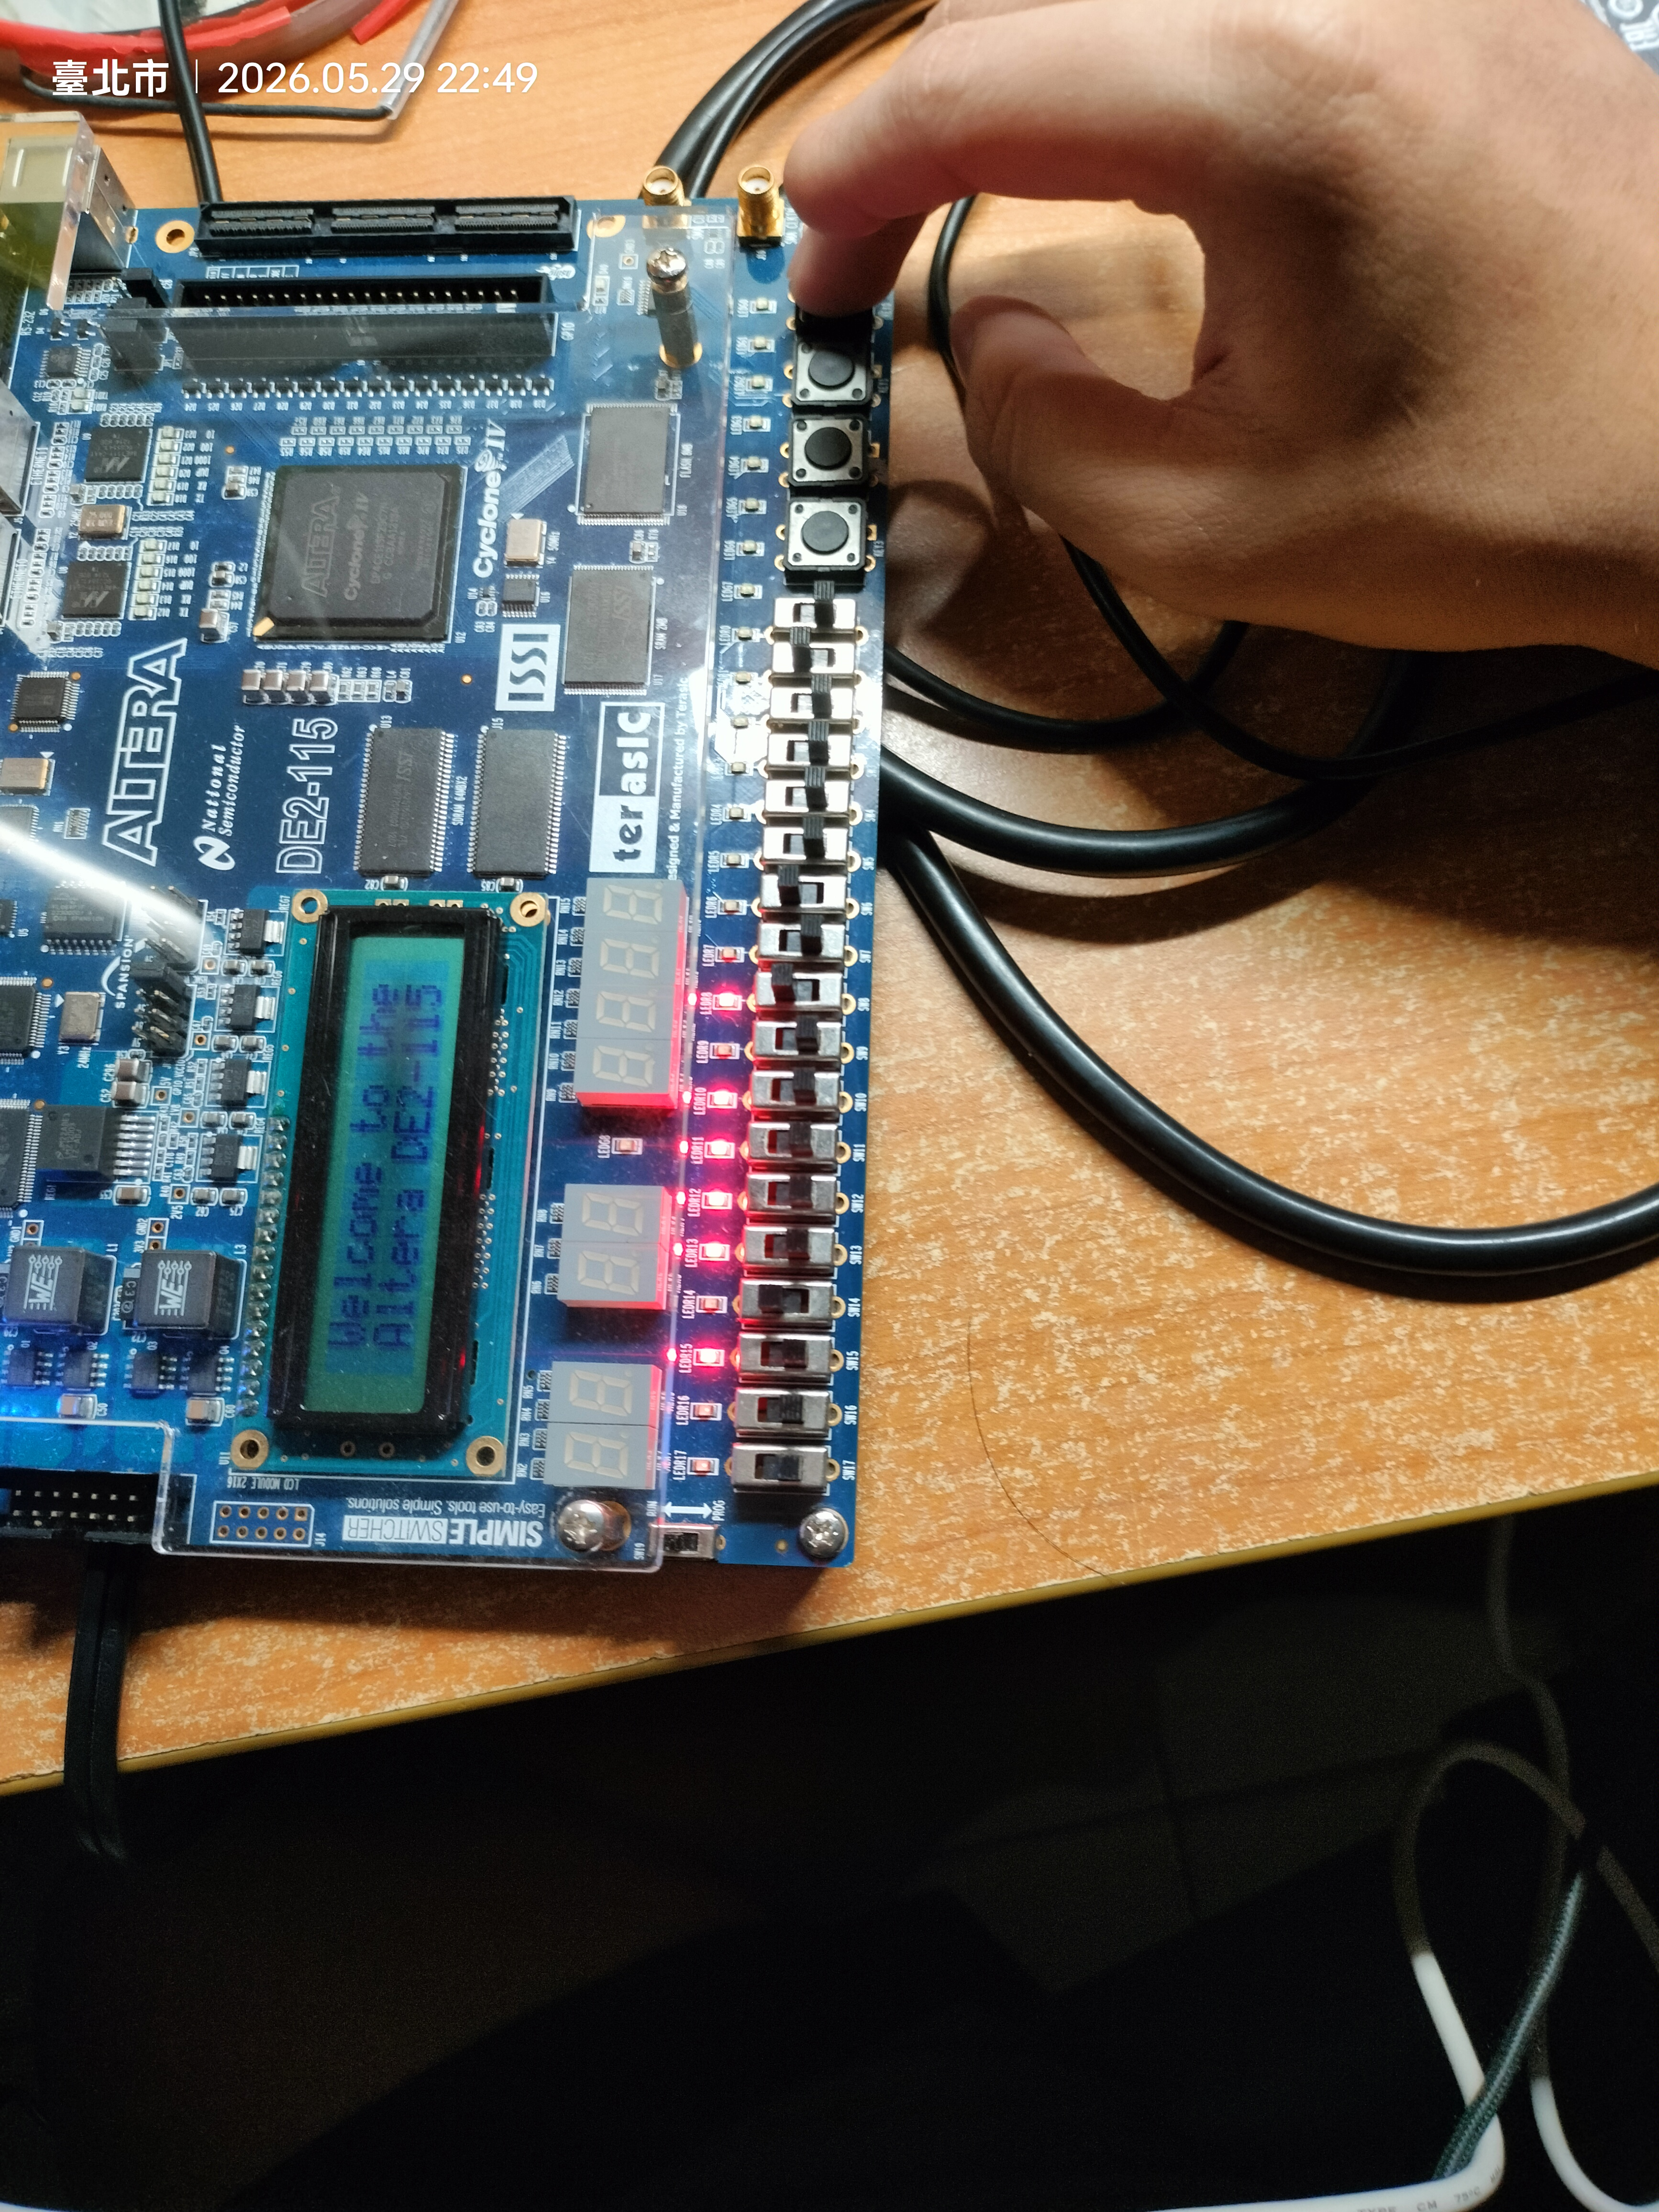
\includegraphics[width=0.65\textwidth]{../../photo/IMG20260529224955.jpg}
    \caption{特殊邊界值測試（一）：測試除數與被除數相等的特殊情況，驗證商為 1、餘數為 0。}
\end{figure}

\begin{figure}[H]
    \centering
    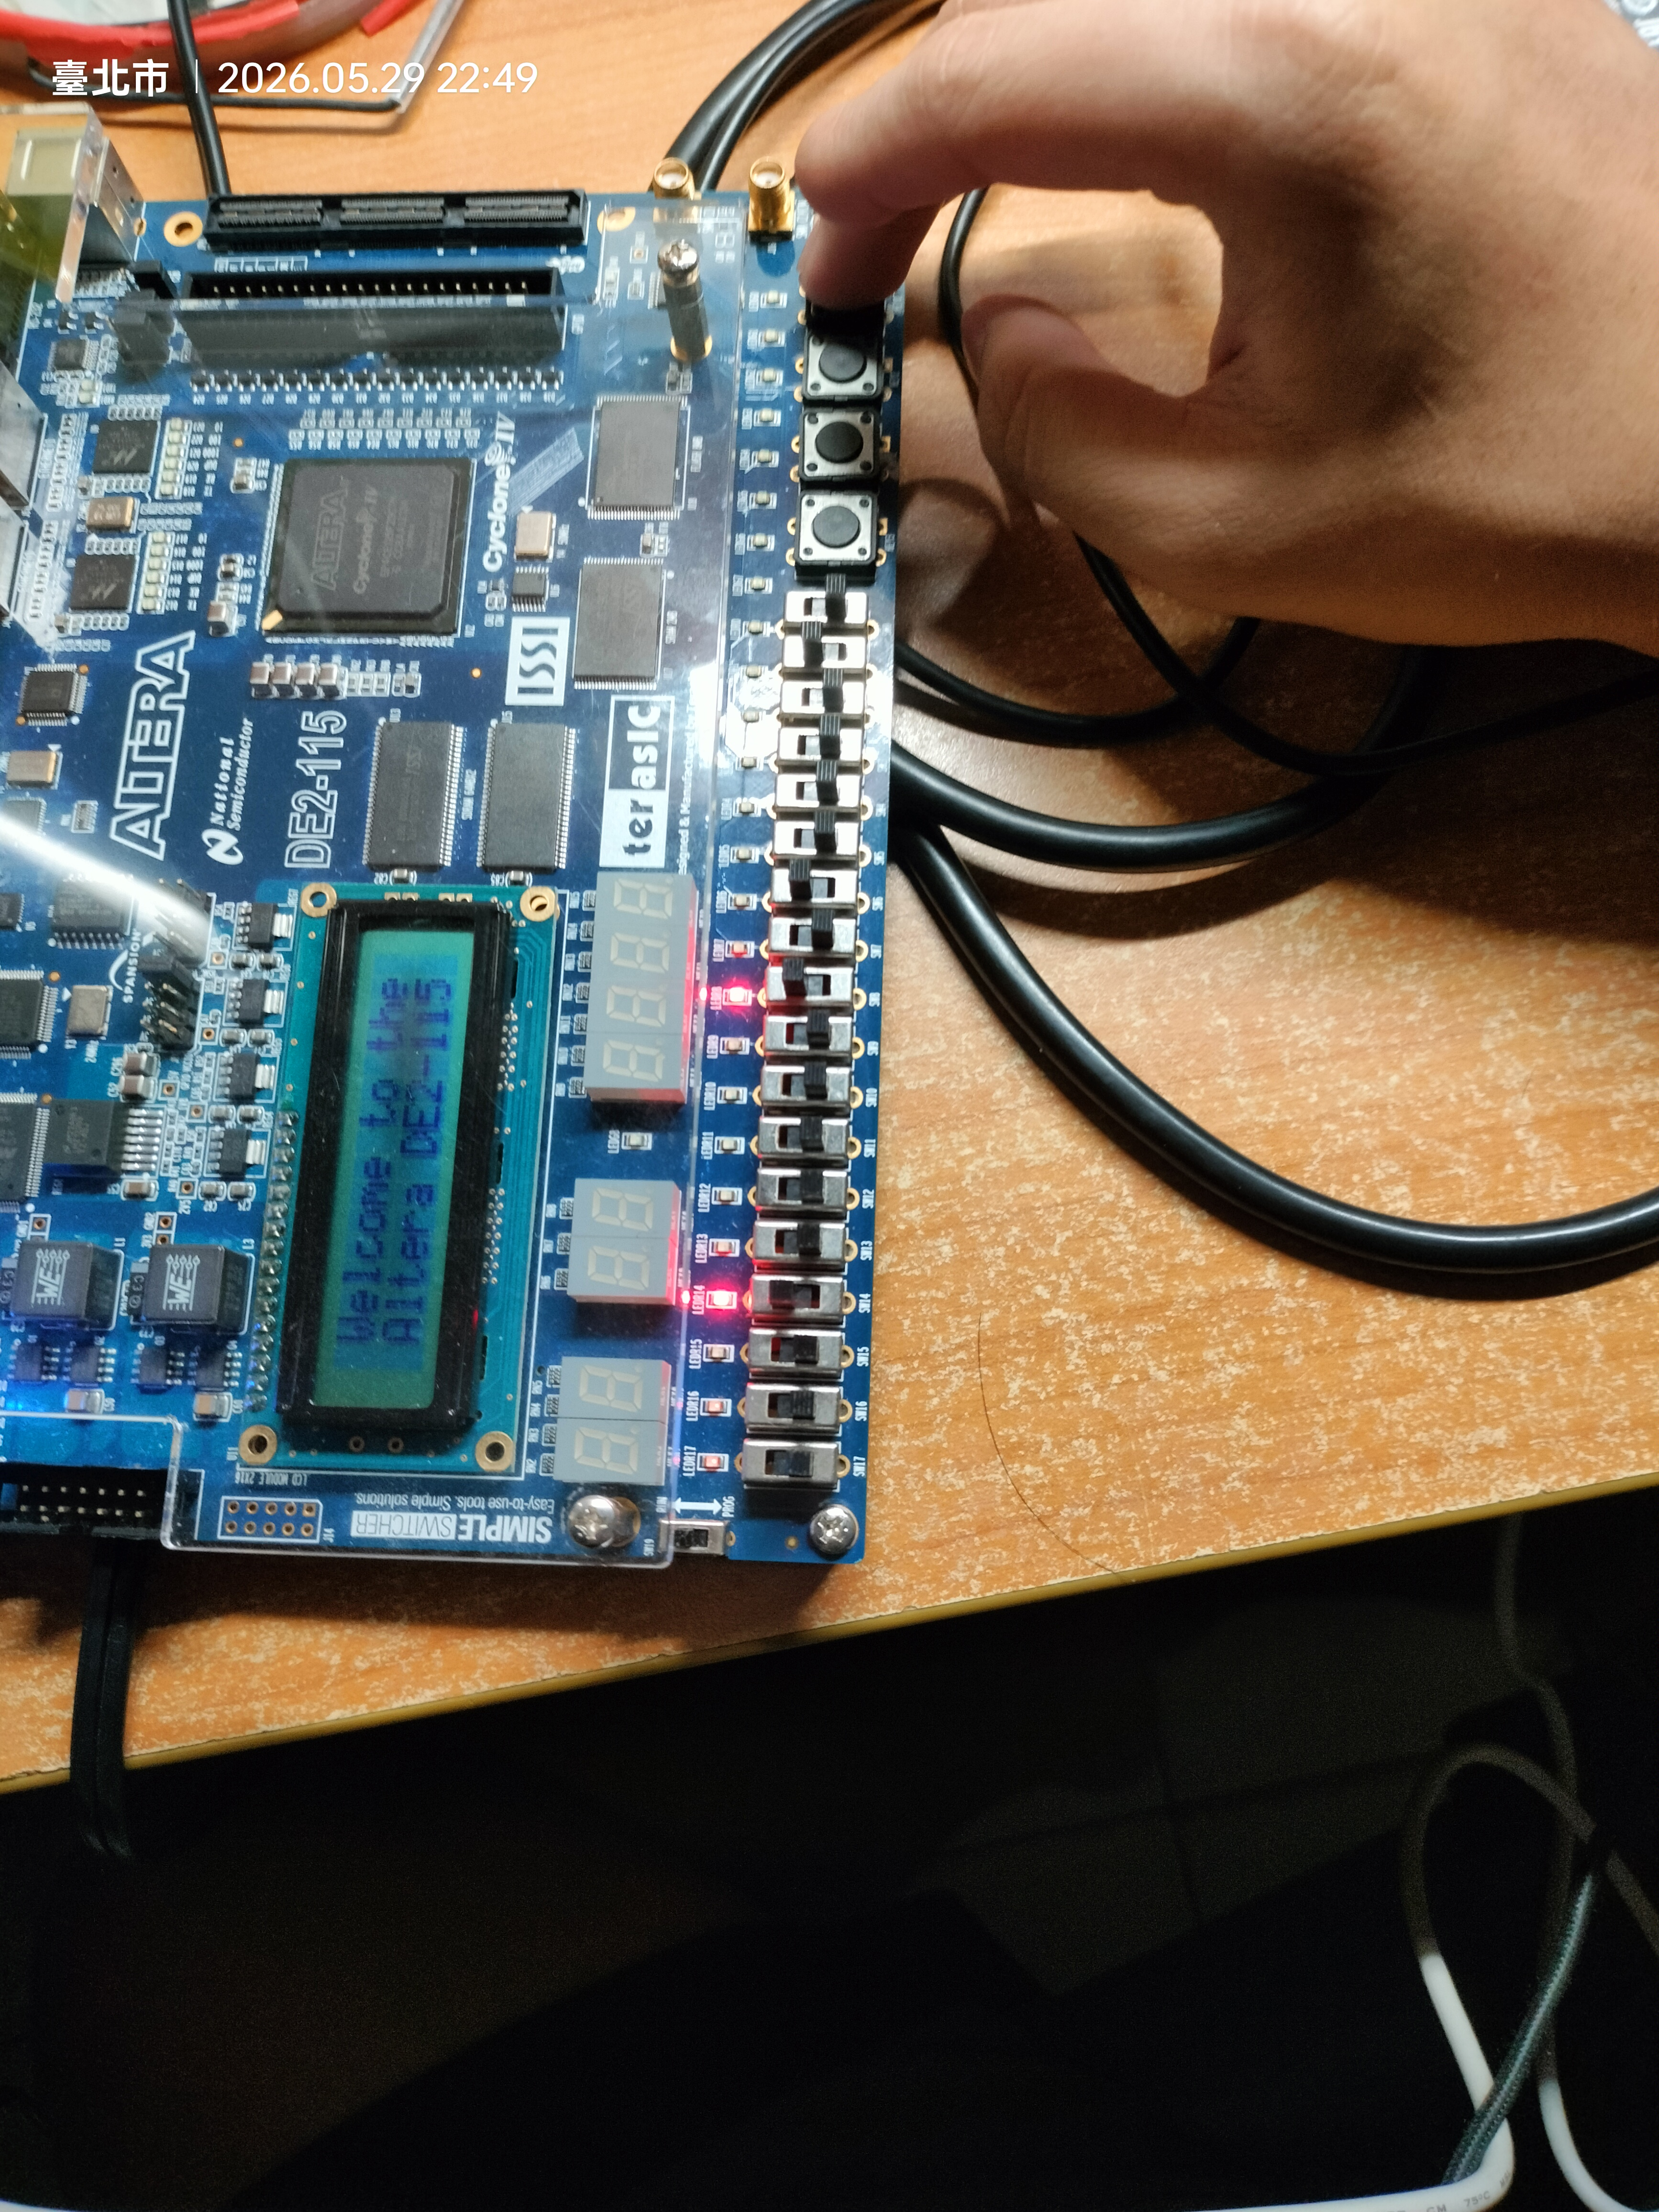
\includegraphics[width=0.65\textwidth]{../../photo/IMG20260529224956.jpg}
    \caption{特殊邊界值測試（二）：七段顯示器顯示 HEX1:HEX0 = 0100（商 4），驗證結果正確。}
\end{figure}

\begin{figure}[H]
    \centering
    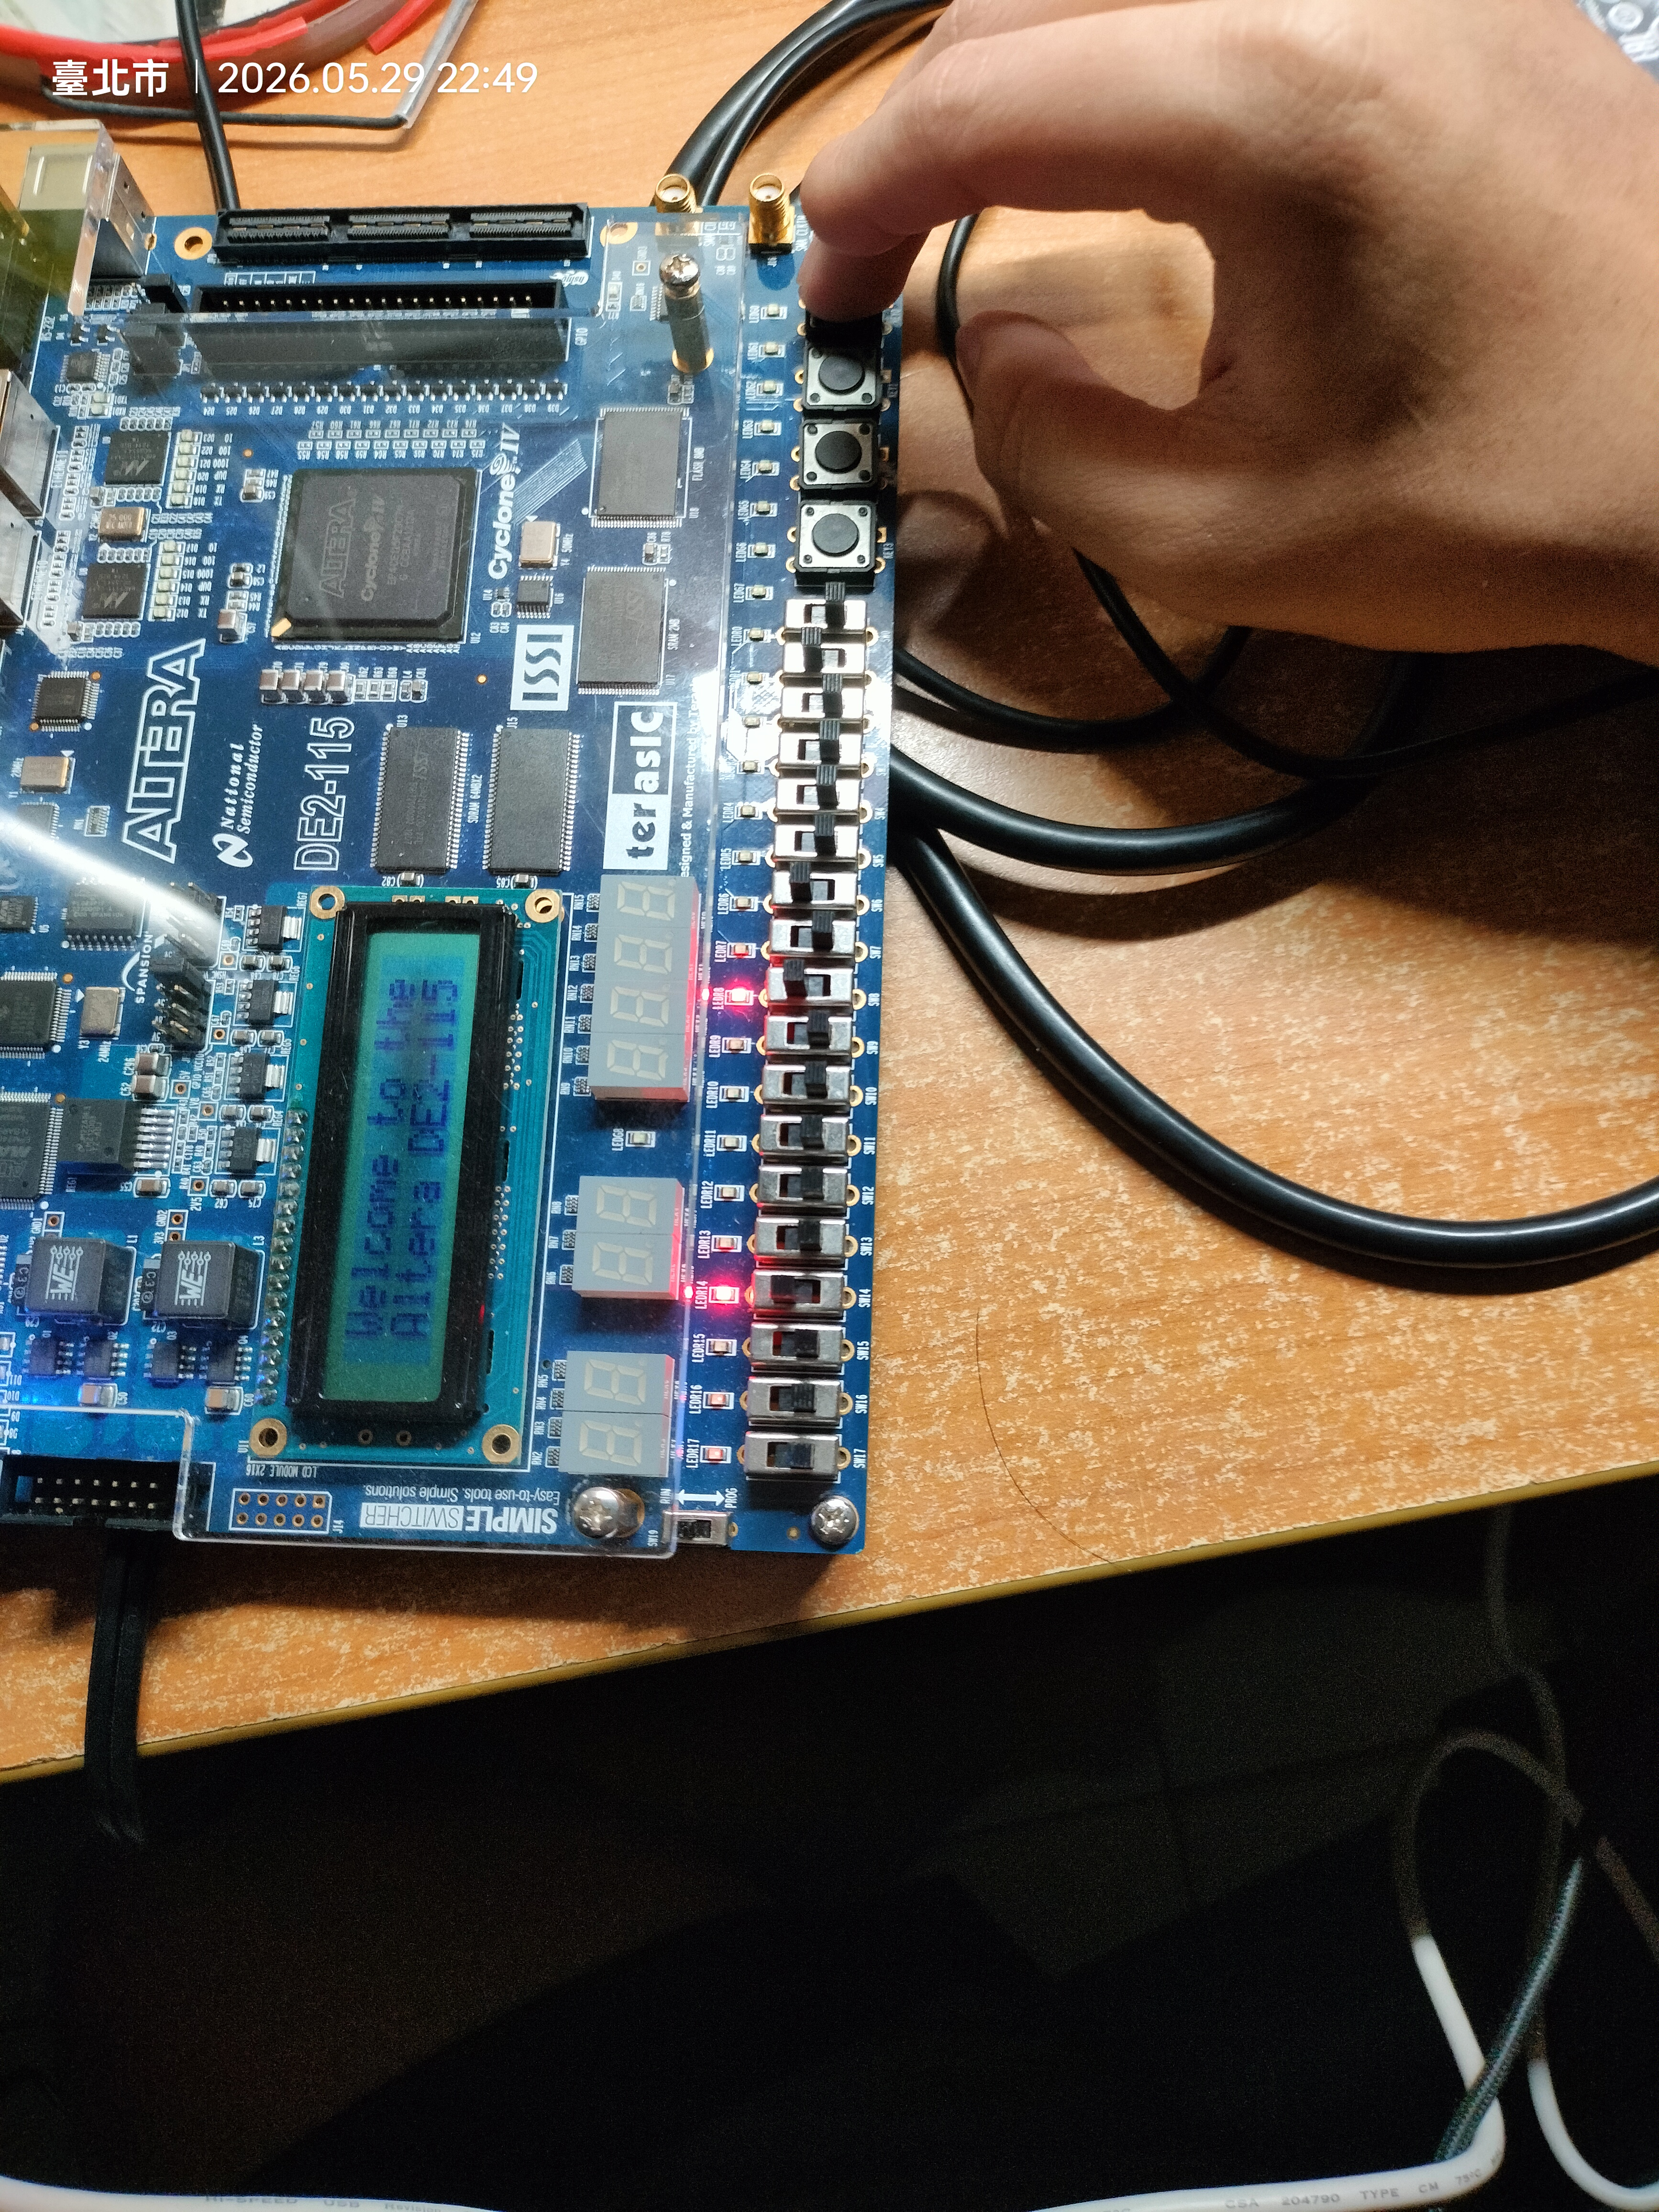
\includegraphics[width=0.65\textwidth]{../../photo/IMG20260529224958.jpg}
    \caption{整體驗證完成（近距離）：清晰可見七段顯示器上的最終商與餘數讀值。}
\end{figure}

\begin{figure}[H]
    \centering
    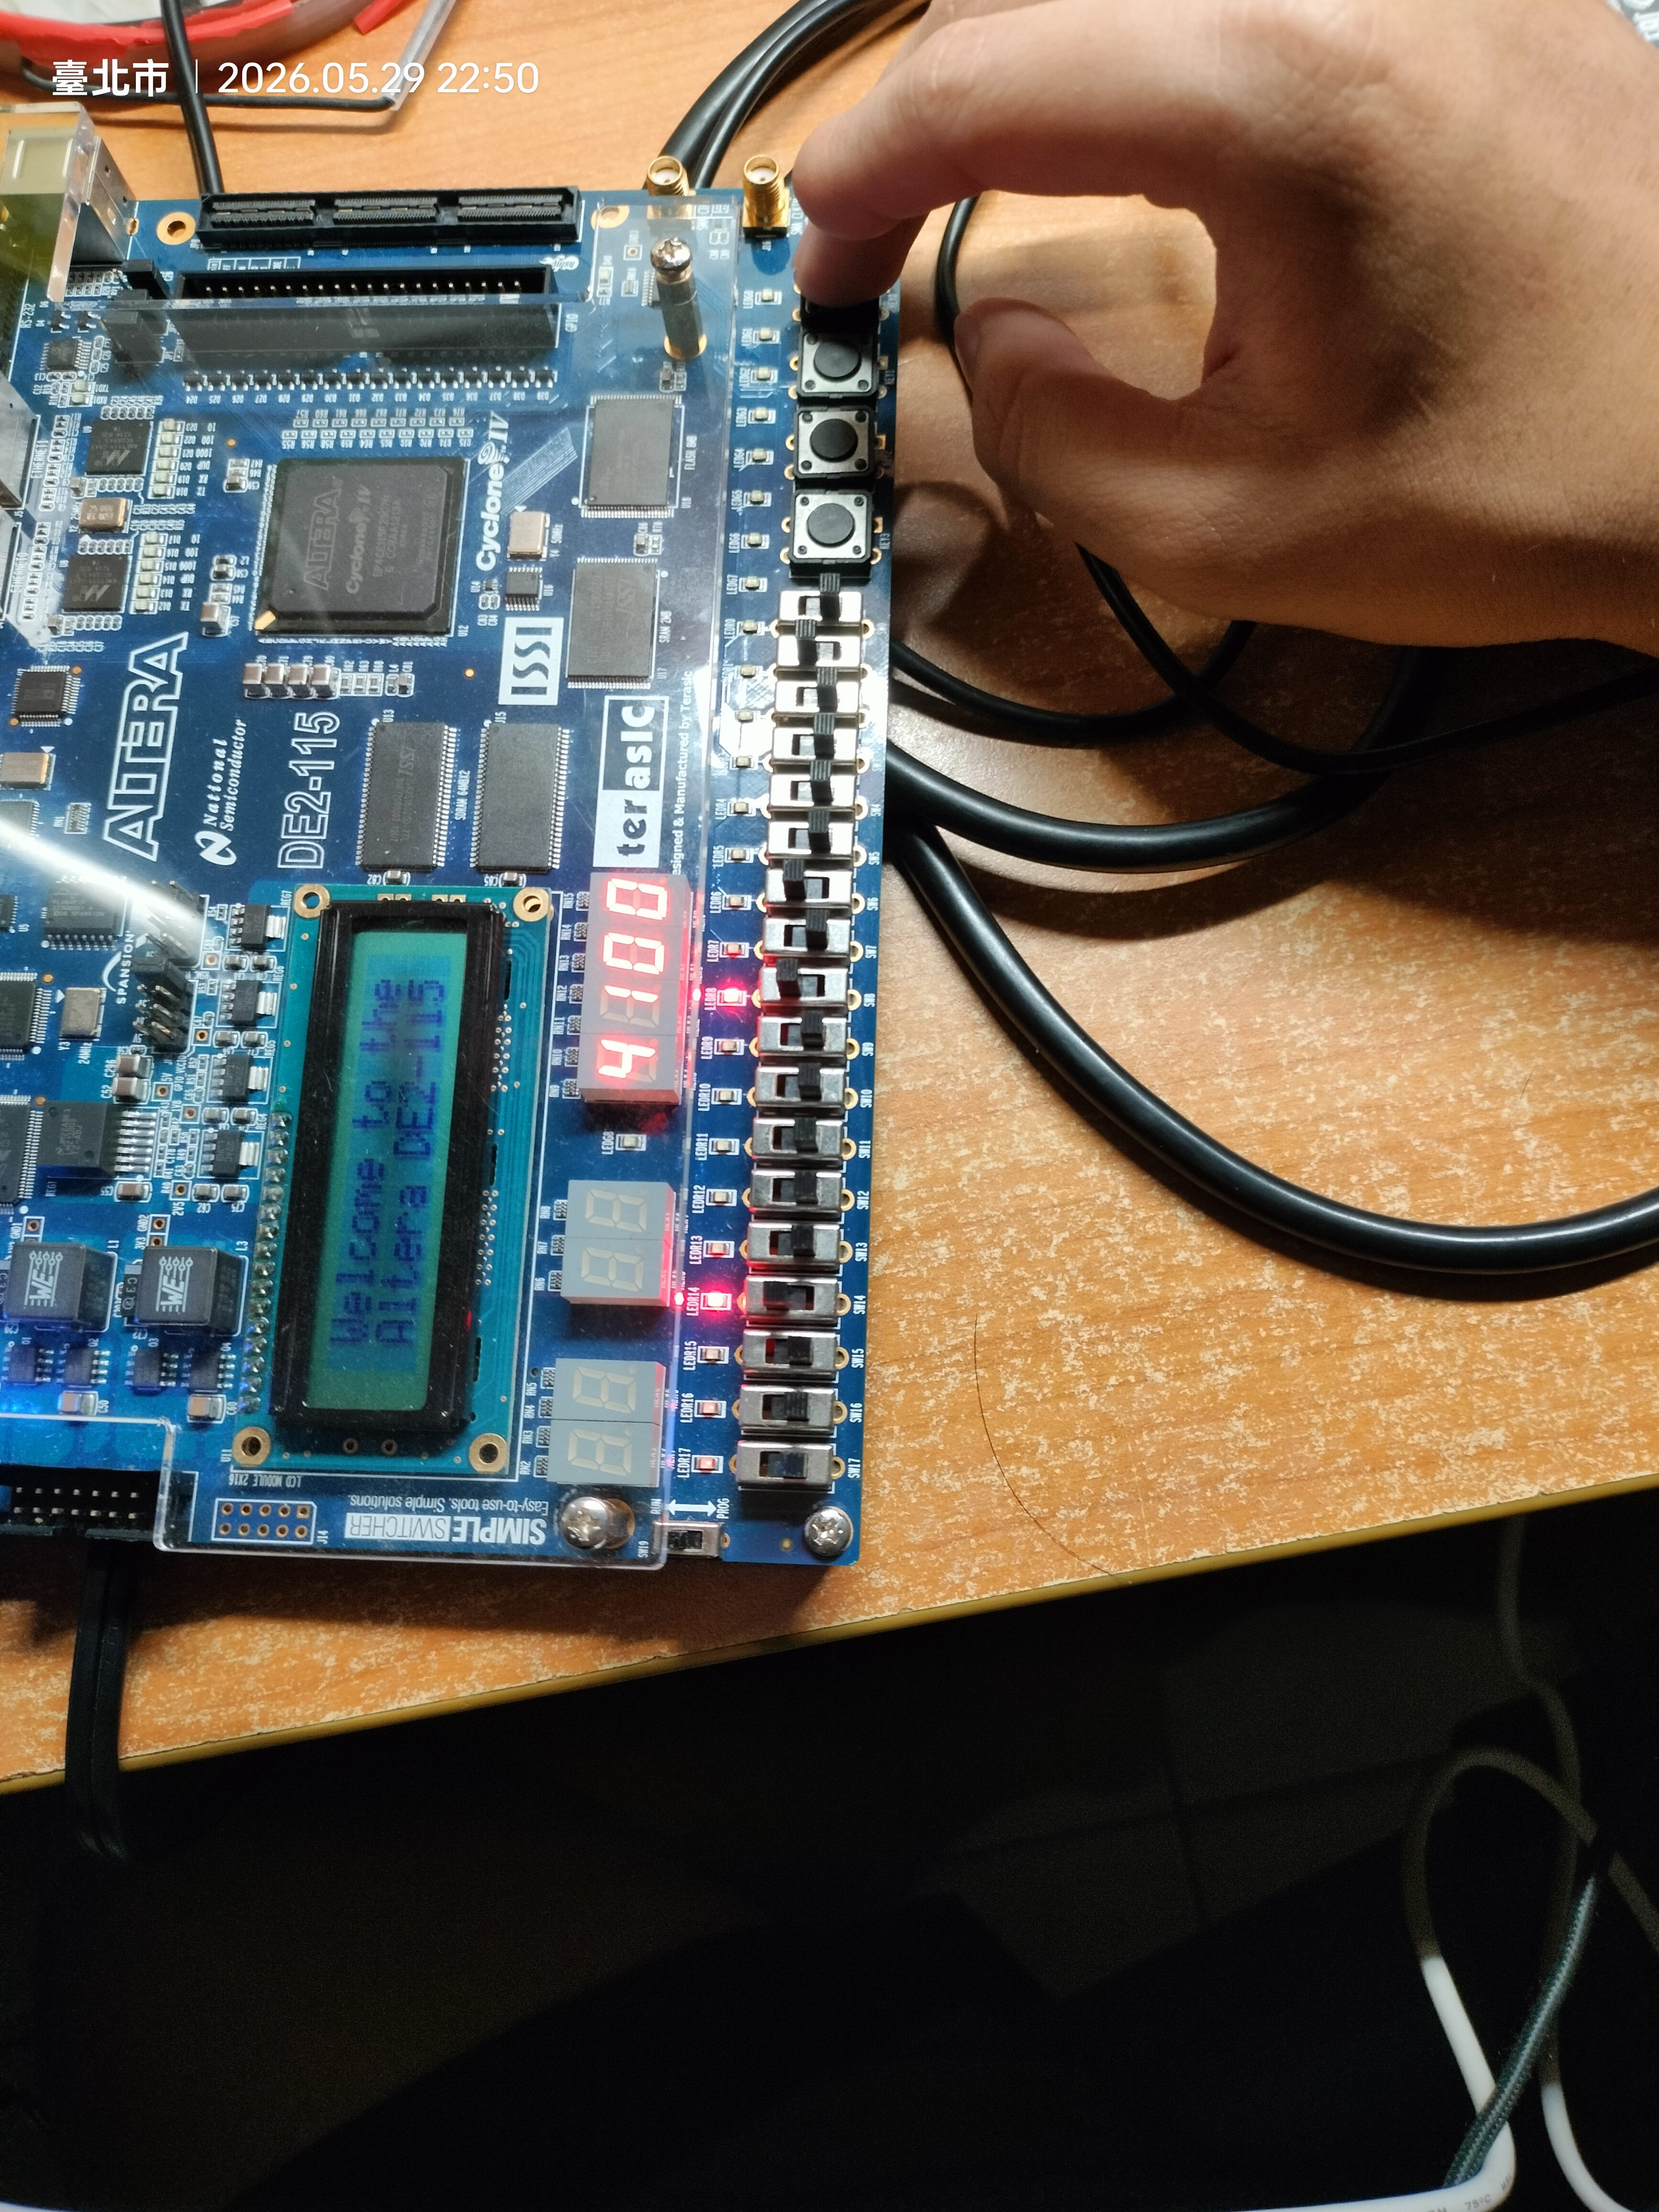
\includegraphics[width=0.65\textwidth]{../../photo/IMG20260529225000.jpg}
    \caption{最終驗證照（全板面）：開發板運作正常，LED 與七段顯示器均呈現正確計算結果，實驗圓滿完成。}
\end{figure}

\newpage

\section{實驗心得}

在本次 Lab 07 的實驗中，我們以「結構化 (Structural)」架構設計了一個完整的 8 位元恢復除法器 (8-Bit Restoring Divider)。相較於 Lab 06 單純實作 FSM 控制器，本次實驗更全面地整合了資料路徑 (Datapath) 與控制器 (Controller) 兩大核心部分，是對 VHDL 硬體描述語言更深一層的實踐。

實驗最重要的設計亮點在於：直接重複使用 Lab 05 所設計的泛用移位暫存器 (\texttt{N\_bit\_DFF})，透過 VHDL 的 \texttt{generic map} 機制，分別實例化出 8-bit 的商數暫存器 (Q)、以及 17-bit 的除數暫存器 (D) 與餘數暫存器 (R)。這讓我們深刻體會到硬體模組化設計的強大之處：一個設計良好的元件，能夠輕鬆因應不同的位元寬度需求，大幅提升設計的可重用性。

在恢復除法演算法的實作上，六個 FSM 狀態（Start、S1、S2a、S2b、S3、S4）與三個暫存器之間的交互控制是本次實驗最具挑戰性的部分。以 S1 的試減結果的符號位元 (\texttt{sub\_res(16)}) 為判斷依據，動態決定是否需要「恢復」餘數（S2b 的 \texttt{R = R + D} 操作），這個設計讓我們對於硬體如何實現條件判斷有了更具體的認識。

在硬體驗證階段，我們利用開發板上的 LED 與七段顯示器進行逐步驗證。由於 KEY[0] 作為手動步進時脈，我們能夠清楚地觀察到每個時脈觸發後各暫存器狀態的即時變化，這種直觀的驗證方式不僅加深了我們對演算法流程的理解，也讓我們成功確認了最終結果的正確性。

\newpage

\section{程式碼 (Division.vhd)}

\begin{lstlisting}[style=vhdlstyle, caption={Division.vhd --- 8-bit 恢復除法器頂層模組（結構化架構）}]
--------------------------------------------------------------------------------
-- Course: Microprocessor Systems (2026)
-- Laboratory: Lab 07 - 8-Bit Restoring Division Hardware Design (Structural)
-- Author: Yang Cheng-Yu / Student ID: 113590051
-- File: Division.vhd
--------------------------------------------------------------------------------

library ieee;
use ieee.std_logic_1164.all;
use ieee.std_logic_unsigned.all;

entity Division is
    port(
        Clock     : in  std_logic;
        Reset     : in  std_logic;
        Divisor   : in  std_logic_vector(7 downto 0);
        Dividend  : in  std_logic_vector(7 downto 0);
        Quotient  : out std_logic_vector(7 downto 0);
        Remainder : out std_logic_vector(7 downto 0);
        HEX0      : out std_logic_vector(6 downto 0);
        HEX1      : out std_logic_vector(6 downto 0);
        HEX2      : out std_logic_vector(6 downto 0);
        HEX3      : out std_logic_vector(6 downto 0)
    );
end entity Division;

architecture Structural of Division is

    component n_bit_DFF is
        generic( N : integer := 10 );
        port(
            clk    : in  std_logic;
            clean  : in  std_logic;
            load   : in  std_logic;
            lr_sel : in  std_logic;
            di     : in  std_logic_vector(N-1 downto 0);
            sdi    : in  std_logic;
            qo     : out std_logic_vector(N-1 downto 0)
        );
    end component;

    type state_type is (Start, S1, S2a, S2b, S3, S4);
    signal current_state : state_type := Start;
    signal count         : integer range 0 to 9 := 0;

    signal clean_Q, load_Q, lr_sel_Q, sdi_Q : std_logic;
    signal di_Q : std_logic_vector(7 downto 0);
    signal qo_Q : std_logic_vector(7 downto 0);

    signal clean_D, load_D, lr_sel_D, sdi_D : std_logic;
    signal di_D : std_logic_vector(16 downto 0);
    signal qo_D : std_logic_vector(16 downto 0);

    signal clean_R, load_R, lr_sel_R, sdi_R : std_logic;
    signal di_R : std_logic_vector(16 downto 0);
    signal qo_R : std_logic_vector(16 downto 0);

    signal sub_res : std_logic_vector(16 downto 0);

    function to_seven_seg(nibble : std_logic_vector(3 downto 0))
      return std_logic_vector is
    begin
        case nibble is
            when "0000" => return "1000000"; -- 0
            when "0001" => return "1111001"; -- 1
            when "0010" => return "0100100"; -- 2
            when "0011" => return "0110000"; -- 3
            when "0100" => return "0011001"; -- 4
            when "0101" => return "0010010"; -- 5
            when "0110" => return "0000010"; -- 6
            when "0111" => return "1111000"; -- 7
            when "1000" => return "0000000"; -- 8
            when "1001" => return "0010000"; -- 9
            when "1010" => return "0001000"; -- A
            when "1011" => return "0000011"; -- b
            when "1100" => return "1000110"; -- C
            when "1101" => return "0100001"; -- d
            when "1110" => return "0000110"; -- E
            when "1111" => return "0001110"; -- F
            when others => return "1111111"; -- Blank
        end case;
    end function;

begin

    reg_Q_inst : n_bit_DFF
        generic map( N => 8 )
        port map( clk=>Clock, clean=>clean_Q, load=>load_Q,
                  lr_sel=>lr_sel_Q, di=>di_Q, sdi=>sdi_Q, qo=>qo_Q );

    reg_D_inst : n_bit_DFF
        generic map( N => 17 )
        port map( clk=>Clock, clean=>clean_D, load=>load_D,
                  lr_sel=>lr_sel_D, di=>di_D, sdi=>sdi_D, qo=>qo_D );

    reg_R_inst : n_bit_DFF
        generic map( N => 17 )
        port map( clk=>Clock, clean=>clean_R, load=>load_R,
                  lr_sel=>lr_sel_R, di=>di_R, sdi=>sdi_R, qo=>qo_R );

    sub_res   <= qo_R - qo_D;
    Quotient  <= qo_Q;
    Remainder <= qo_R(7 downto 0);

    process(current_state, Dividend, Divisor, qo_Q, qo_D, qo_R, sub_res)
    begin
        clean_Q<='0'; load_Q<='1'; lr_sel_Q<='1'; sdi_Q<='0'; di_Q<=qo_Q;
        clean_D<='0'; load_D<='1'; lr_sel_D<='0'; sdi_D<='0'; di_D<=qo_D;
        clean_R<='0'; load_R<='1'; lr_sel_R<='1'; sdi_R<='0'; di_R<=qo_R;

        case current_state is
            when Start =>
                clean_Q <= '1';  load_Q <= '0';
                load_D  <= '1';  di_D   <= '0' & Divisor & "00000000";
                load_R  <= '1';  di_R   <= "000000000" & Dividend;
            when S1 =>
                load_R <= '1';   di_R   <= sub_res;
            when S2a =>
                load_Q <= '0';   lr_sel_Q <= '1'; sdi_Q <= '1';
            when S2b =>
                load_R <= '1';   di_R     <= qo_R + qo_D;
                load_Q <= '0';   lr_sel_Q <= '1'; sdi_Q <= '0';
            when S3 =>
                load_D <= '0';   lr_sel_D <= '0'; sdi_D <= '0';
            when S4 =>
                null;
        end case;
    end process;

    process(Clock, Reset)
    begin
        if Reset = '1' then
            current_state <= Start;  count <= 0;
        elsif rising_edge(Clock) then
            case current_state is
                when Start => count <= 0;  current_state <= S1;
                when S1 =>
                    if sub_res(16) = '0' then current_state <= S2a;
                    else                       current_state <= S2b; end if;
                when S2a => current_state <= S3;
                when S2b => current_state <= S3;
                when S3  =>
                    if count = 8 then current_state <= S4;
                    else count <= count + 1; current_state <= S1; end if;
                when S4  => current_state <= S4;
            end case;
        end if;
    end process;

    process(current_state, qo_Q, qo_R)
    begin
        if current_state = S4 then
            HEX0 <= to_seven_seg(qo_Q(3 downto 0));
            HEX1 <= to_seven_seg(qo_Q(7 downto 4));
            HEX2 <= to_seven_seg(qo_R(3 downto 0));
            HEX3 <= to_seven_seg(qo_R(7 downto 4));
        else
            HEX0 <= (others => '1');  HEX1 <= (others => '1');
            HEX2 <= (others => '1');  HEX3 <= (others => '1');
        end if;
    end process;

end architecture Structural;
\end{lstlisting}

\newpage

\section{程式碼 (N\_bit\_DFF.vhd)}

\begin{lstlisting}[style=vhdlstyle, caption={N\_bit\_DFF.vhd --- 泛用 N-bit 移位暫存器元件（重用自 Lab 05）}]
--------------------------------------------------------------------------------
-- Course: Microprocessor Systems (2026)
-- Laboratory: Lab 07 - Multi-Purpose Shift Register (Reused from Lab 05)
-- File: N_bit_DFF.vhd
--------------------------------------------------------------------------------

library ieee;
use ieee.std_logic_1164.all;
use ieee.std_logic_unsigned.all;

entity n_bit_DFF is
    generic( N : integer := 10 );
    port(
        clk    : in  std_logic;
        clean  : in  std_logic;
        load   : in  std_logic;
        lr_sel : in  std_logic;
        di     : in  std_logic_vector(N-1 downto 0);
        sdi    : in  std_logic;
        qo     : out std_logic_vector(N-1 downto 0)
    );
end entity n_bit_DFF;

architecture Behavioral of n_bit_DFF is
    signal reg : std_logic_vector(N-1 downto 0) := (others => '0');
begin
    process(clk)
    begin
        if rising_edge(clk) then
            if clean = '1' then
                reg <= (others => '0');
            elsif load = '1' then
                reg <= di;
            elsif lr_sel = '1' then
                -- Left shift: reg(N-1) <- reg(N-2) <- ... <- reg(0) <- sdi
                for i in N-1 downto 1 loop
                    reg(i) <= reg(i-1);
                end loop;
                reg(0) <= sdi;
            elsif lr_sel = '0' then
                -- Right shift: reg(0) -> reg(1) -> ... -> reg(N-1) -> sdi
                for i in 0 to N-2 loop
                    reg(i) <= reg(i+1);
                end loop;
                reg(N-1) <= sdi;
            end if;
        end if;
    end process;

    qo <= reg;

end architecture Behavioral;
\end{lstlisting}

\end{document}
